\documentclass[a4paper]{article}

\def\npart {IB}
\def\nterm {Lent}
\def\nyear {2016}
\def\nlecturer {O.\ Randal-Williams}
\def\ncourse {Groups, Rings and Modules}

% Imports
\ifx \nextra \undefined
  \usepackage[pdftex,
    hidelinks,
    pdfauthor={Dexter Chua},
    pdfsubject={Cambridge Maths Notes: Part \npart\ - \ncourse},
    pdftitle={Part \npart\ - \ncourse},
  pdfkeywords={Cambridge Mathematics Maths Math \npart\ \nterm\ \nyear\ \ncourse}]{hyperref}
  \title{Part \npart\ - \ncourse}
\else
  \usepackage[pdftex,
    hidelinks,
    pdfauthor={Dexter Chua},
    pdfsubject={Cambridge Maths Notes: Part \npart\ - \ncourse\ (\nextra)},
    pdftitle={Part \npart\ - \ncourse\ (\nextra)},
  pdfkeywords={Cambridge Mathematics Maths Math \npart\ \nterm\ \nyear\ \ncourse\ \nextra}]{hyperref}

  \title{Part \npart\ - \ncourse \\ {\Large \nextra}}
\fi

\author{Lectured by \nlecturer \\\small Notes taken by Dexter Chua}
\date{\nterm\ \nyear}

\usepackage{alltt}
\usepackage{amsfonts}
\usepackage{amsmath}
\usepackage{amssymb}
\usepackage{amsthm}
\usepackage{booktabs}
\usepackage{caption}
\usepackage{enumitem}
\usepackage{fancyhdr}
\usepackage{graphicx}
\usepackage{mathtools}
\usepackage{microtype}
\usepackage{multirow}
\usepackage{pdflscape}
\usepackage{pgfplots}
\usepackage{siunitx}
\usepackage{tabularx}
\usepackage{tikz}
\usepackage{tkz-euclide}
\usepackage[normalem]{ulem}
\usepackage[all]{xy}

\pgfplotsset{compat=1.12}

\pagestyle{fancyplain}
\lhead{\emph{\nouppercase{\leftmark}}}
\ifx \nextra \undefined
  \rhead{
    \ifnum\thepage=1
    \else
      \npart\ \ncourse
    \fi}
\else
  \rhead{
    \ifnum\thepage=1
    \else
      \npart\ \ncourse\ (\nextra)
    \fi}
\fi
\usetikzlibrary{arrows}
\usetikzlibrary{decorations.markings}
\usetikzlibrary{decorations.pathmorphing}
\usetikzlibrary{positioning}
\usetikzlibrary{fadings}
\usetikzlibrary{intersections}
\usetikzlibrary{cd}

\newcommand*{\Cdot}{\raisebox{-0.25ex}{\scalebox{1.5}{$\cdot$}}}
\newcommand {\pd}[2][ ]{
  \ifx #1 { }
    \frac{\partial}{\partial #2}
  \else
    \frac{\partial^{#1}}{\partial #2^{#1}}
  \fi
}

% Theorems
\theoremstyle{definition}
\newtheorem*{aim}{Aim}
\newtheorem*{axiom}{Axiom}
\newtheorem*{claim}{Claim}
\newtheorem*{cor}{Corollary}
\newtheorem*{defi}{Definition}
\newtheorem*{eg}{Example}
\newtheorem*{fact}{Fact}
\newtheorem*{law}{Law}
\newtheorem*{lemma}{Lemma}
\newtheorem*{notation}{Notation}
\newtheorem*{prop}{Proposition}
\newtheorem*{thm}{Theorem}

\renewcommand{\labelitemi}{--}
\renewcommand{\labelitemii}{$\circ$}
\renewcommand{\labelenumi}{(\roman{*})}

\let\stdsection\section
\renewcommand\section{\newpage\stdsection}

% Strike through
\def\st{\bgroup \ULdepth=-.55ex \ULset}

% Maths symbols
\newcommand{\bra}{\langle}
\newcommand{\ket}{\rangle}

\newcommand{\N}{\mathbb{N}}
\newcommand{\Z}{\mathbb{Z}}
\newcommand{\Q}{\mathbb{Q}}
\renewcommand{\H}{\mathbb{H}}
\newcommand{\R}{\mathbb{R}}
\newcommand{\C}{\mathbb{C}}
\newcommand{\Prob}{\mathbb{P}}
\renewcommand{\P}{\mathbb{P}}
\newcommand{\E}{\mathbb{E}}
\newcommand{\F}{\mathbb{F}}
\newcommand{\cU}{\mathcal{U}}
\newcommand{\RP}{\mathbb{RP}}
\newcommand{\CP}{\mathbb{CP}}

\newcommand{\ph}{\,\cdot\,}

\DeclareMathOperator{\sech}{sech}
\DeclareMathOperator{\cosech}{cosech}
\DeclareMathOperator{\cosec}{cosec}

\DeclareMathOperator{\covol}{covol}
\DeclareMathOperator{\vol}{vol}

\let\Im\relax
\let\Re\relax
\DeclareMathOperator{\Im}{Im}
\DeclareMathOperator{\Re}{Re}
\DeclareMathOperator{\im}{im}
\DeclareMathOperator{\image}{image}
\DeclareMathOperator{\Ann}{Ann}

\DeclareMathOperator*{\res}{res}
\DeclareMathOperator{\Res}{Res}
\DeclareMathOperator{\Ind}{Ind}

\DeclareMathOperator{\tr}{tr}
\DeclareMathOperator{\diag}{diag}
\DeclareMathOperator{\rank}{rank}
\DeclareMathOperator{\card}{card}
\DeclareMathOperator{\spn}{span}
\DeclareMathOperator{\adj}{adj}

\DeclareMathOperator{\erf}{erf}
\DeclareMathOperator{\erfc}{erfc}

\DeclareMathOperator{\ord}{ord}
\DeclareMathOperator{\Sym}{Sym}

\DeclareMathOperator{\sgn}{sgn}
\DeclareMathOperator{\orb}{orb}
\DeclareMathOperator{\stab}{stab}
\DeclareMathOperator{\ccl}{ccl}

\DeclareMathOperator{\lcm}{lcm}
\DeclareMathOperator{\hcf}{hcf}

\DeclareMathOperator{\Int}{Int}
\DeclareMathOperator{\id}{id}

\DeclareMathOperator{\betaD}{beta}
\DeclareMathOperator{\gammaD}{gamma}
\DeclareMathOperator{\Poisson}{Poisson}
\DeclareMathOperator{\binomial}{binomial}
\DeclareMathOperator{\multinomial}{multinomial}
\DeclareMathOperator{\Bernoulli}{Bernoulli}
\DeclareMathOperator{\like}{like}

\DeclareMathOperator{\var}{var}
\DeclareMathOperator{\cov}{cov}
\DeclareMathOperator{\bias}{bias}
\DeclareMathOperator{\mse}{mse}
\DeclareMathOperator{\corr}{corr}

\DeclareMathOperator{\otp}{otp}
\DeclareMathOperator{\dom}{dom}

\DeclareMathOperator{\Root}{Root}
\DeclareMathOperator{\supp}{supp}
\DeclareMathOperator{\rel}{rel}
\DeclareMathOperator{\Hom}{Hom}
\DeclareMathOperator{\Aut}{Aut}
\DeclareMathOperator{\Gal}{Gal}
\DeclareMathOperator{\Mat}{Mat}
\DeclareMathOperator{\End}{End}
\DeclareMathOperator{\Char}{char}
\DeclareMathOperator{\ev}{ev}
\DeclareMathOperator{\St}{St}
\DeclareMathOperator{\Lk}{Lk}
\DeclareMathOperator{\disc}{disc}
\DeclareMathOperator{\Isom}{Isom}
\DeclareMathOperator{\length}{length}
\DeclareMathOperator{\energy}{energy}
\DeclareMathOperator{\area}{area}
\DeclareMathOperator{\Syl}{Syl}
\DeclareMathOperator{\cl}{cl}
\DeclareMathOperator{\fix}{fix}

\newcommand{\GL}{\mathrm{GL}}
\newcommand{\SL}{\mathrm{SL}}
\newcommand{\PGL}{\mathrm{PGL}}
\newcommand{\PSL}{\mathrm{PSL}}
\newcommand{\PSU}{\mathrm{PSU}}
\newcommand{\Or}{\mathrm{O}}
\newcommand{\SO}{\mathrm{SO}}
\newcommand{\U}{\mathrm{U}}
\newcommand{\SU}{\mathrm{SU}}

\renewcommand{\d}{\mathrm{d}}
\newcommand{\D}{\mathrm{D}}

\tikzset{->/.style = {decoration={markings,
                                  mark=at position 1 with {\arrow[scale=2]{latex'}}},
                      postaction={decorate}}}
\tikzset{<-/.style = {decoration={markings,
                                  mark=at position 0 with {\arrowreversed[scale=2]{latex'}}},
                      postaction={decorate}}}
\tikzset{<->/.style = {decoration={markings,
                                   mark=at position 0 with {\arrowreversed[scale=2]{latex'}},
                                   mark=at position 1 with {\arrow[scale=2]{latex'}}},
                       postaction={decorate}}}
\tikzset{->-/.style = {decoration={markings,
                                   mark=at position #1 with {\arrow[scale=2]{latex'}}},
                       postaction={decorate}}}
\tikzset{-<-/.style = {decoration={markings,
                                   mark=at position #1 with {\arrowreversed[scale=2]{latex'}}},
                       postaction={decorate}}}

\tikzset{circ/.style = {fill, circle, inner sep = 0, minimum size = 3}}
\tikzset{mstate/.style={circle, draw, blue, text=black, minimum width=0.7cm}}

\definecolor{mblue}{rgb}{0.2, 0.3, 0.8}
\definecolor{morange}{rgb}{1, 0.5, 0}
\definecolor{mgreen}{rgb}{0.1, 0.4, 0.2}
\definecolor{mred}{rgb}{0.5, 0, 0}

\def\drawcirculararc(#1,#2)(#3,#4)(#5,#6){%
    \pgfmathsetmacro\cA{(#1*#1+#2*#2-#3*#3-#4*#4)/2}%
    \pgfmathsetmacro\cB{(#1*#1+#2*#2-#5*#5-#6*#6)/2}%
    \pgfmathsetmacro\cy{(\cB*(#1-#3)-\cA*(#1-#5))/%
                        ((#2-#6)*(#1-#3)-(#2-#4)*(#1-#5))}%
    \pgfmathsetmacro\cx{(\cA-\cy*(#2-#4))/(#1-#3)}%
    \pgfmathsetmacro\cr{sqrt((#1-\cx)*(#1-\cx)+(#2-\cy)*(#2-\cy))}%
    \pgfmathsetmacro\cA{atan2(#2-\cy,#1-\cx)}%
    \pgfmathsetmacro\cB{atan2(#6-\cy,#5-\cx)}%
    \pgfmathparse{\cB<\cA}%
    \ifnum\pgfmathresult=1
        \pgfmathsetmacro\cB{\cB+360}%
    \fi
    \draw (#1,#2) arc (\cA:\cB:\cr);%
}
\newcommand\getCoord[3]{\newdimen{#1}\newdimen{#2}\pgfextractx{#1}{\pgfpointanchor{#3}{center}}\pgfextracty{#2}{\pgfpointanchor{#3}{center}}}

\def\Xint#1{\mathchoice
   {\XXint\displaystyle\textstyle{#1}}%
   {\XXint\textstyle\scriptstyle{#1}}%
   {\XXint\scriptstyle\scriptscriptstyle{#1}}%
   {\XXint\scriptscriptstyle\scriptscriptstyle{#1}}%
   \!\int}
\def\XXint#1#2#3{{\setbox0=\hbox{$#1{#2#3}{\int}$}
     \vcenter{\hbox{$#2#3$}}\kern-.5\wd0}}
\def\ddashint{\Xint=}
\def\dashint{\Xint-}


\begin{document}
\maketitle
{\small
\noindent\textbf{Groups}\\
Basic concepts of group theory recalled from Part IA Groups. Normal subgroups, quotient groups and isomorphism theorems. Permutation groups. Groups acting on sets, permutation representations. Conjugacy classes, centralizers and normalizers. The centre of a group. Elementary properties of finite $p$-groups. Examples of finite linear groups and groups arising from geometry. Simplicity of $A_n$.

\vspace{5pt}
\noindent Sylow subgroups and Sylow theorems. Applications, groups of small order.\hspace*{\fill} [8]

\vspace{10pt}
\noindent\textbf{Rings}\\
Definition and examples of rings (commutative, with 1). Ideals, homomorphisms, quotient rings, isomorphism theorems. Prime and maximal ideals. Fields. The characteristic of a field. Field of fractions of an integral domain.

\vspace{5pt}
\noindent Factorization in rings; units, primes and irreducibles. Unique factorization in principal ideal domains, and in polynomial rings. Gauss' Lemma and Eisenstein's irreducibility criterion.

\vspace{5pt}
\noindent Rings $\Z[\alpha]$ of algebraic integers as subsets of $\C$ and quotients of $\Z[x]$. Examples of Euclidean domains and uniqueness and non-uniqueness of factorization. Factorization in the ring of Gaussian integers; representation of integers as sums of two squares.

\vspace{5pt}
\noindent Ideals in polynomial rings. Hilbert basis theorem.\hspace*{\fill} [10]

\vspace{10pt}
\noindent\textbf{Modules}\\
Definitions, examples of vector spaces, abelian groups and vector spaces with an endomorphism. Sub-modules, homomorphisms, quotient modules and direct sums. Equivalence of matrices, canonical form. Structure of finitely generated modules over Euclidean domains, applications to abelian groups and Jordan normal form.\hspace*{\fill} [6]}

\tableofcontents
\setcounter{section}{-1}
\section{Introduction}
The course is naturally divided into three sections --- Groups, Rings, and Modules.

In IA Groups, we learnt about some basic properties of groups, and studied several interesting groups in depth. In the first part of this course, we will further develop some general theory of groups. In particular, we will prove two more isomorphism theorems of groups. While we will not find these theorems particularly useful in this course, we will be able to formulate analogous theorems for other algebraic structures such as rings and modules, as we will later find in the course.

In the next part of the course, we will study rings. These are things that behave somewhat like $\Z$, where we can add, subtract, multiply but not (necessarily) divide. While $\Z$ has many nice properties, these are not necessarily available in arbitrary rings. Hence we will classify rings into different types, depending on how many properties of $\Z$ they inherit. We can then try to reconstruct certain IA Numbers and Sets results in these rings, such as unique factorization of numbers into primes and B\'ezout's theorem.

Finally, we move on to modules. The definition of a module is very similar to that of a vector space, except that instead of allowing scalar multiplication by elements of a field, we have scalar multiplication by elements of a ring. It turns out modules are completely unlike vector spaces, and can have much more complicated structures. Perhaps because of this richness, many things turn out to be modules. Using module theory, we will be able to prove certain important theorems such as the classification of finite abelian groups and the Jordan normal form theorem.

\section{Groups}
\subsection{Basic concepts}
We will begin by quickly recapping some definitions and results from IA Groups.

\begin{defi}[Group]\index{group}
  A \emph{group} is a triple $(G, \ph, e)$, where $G$ is a set, $\ph: G\times G \to G$ is a function and $e \in G$ is an element such that
  \begin{enumerate}
    \item For all $a, b, c \in G$, we have $(a \cdot b) \cdot c = a \cdot (b \cdot c)$.\hfill (associativity)
    \item For all $a \in G$, we have $a \cdot e = e \cdot a = a$.\hfill (identity)\index{identity}
    \item For all $a \in G$, there exists $a^{-1} \in G$ such that $a \cdot a^{-1} = a^{-1} \cdot a = e$.\hfill (inverse)\index{inverse}
  \end{enumerate}
\end{defi}
Some people add a stupid axiom that says $g \cdot h \in G$ for all $g, h \in G$, but this is already implied by saying $\cdot$ is a function to $G$. You can write that down as well, and no one will say you are stupid. But they might secretly \emph{think} so.

\begin{lemma}
  The inverse of an element is unique.
\end{lemma}

\begin{proof}
  Let $a^{-1}, b$ be inverses of $a$. Then
  \[
    b = b \cdot e = b \cdot a \cdot a^{-1} = e \cdot a^{-1} = a^{-1}. \qedhere
  \]
\end{proof}

\begin{defi}[Subgroup]
  If $(G, \ph, e)$ is a group and $H \subseteq G$ is a subset, it is a \emph{subgroup} if
  \begin{enumerate}
    \item $e \in H$,
    \item $a, b \in H$ implies $a\cdot b\in H$,
    \item $\ph: H \times H \to H$ makes $(H, \ph, e)$ a group.
  \end{enumerate}
  We write $H \leq G$ if $H$ is a subgroup of $G$.
\end{defi}
Note that the last condition in some sense encompasses the first two, but we need the first two conditions to hold before the last statement makes sense at all.

\begin{lemma}
  $H \subseteq G$ is a subgroup if $H$ is non-empty and for any $h_1, h_2 \in H$, we have $h_1h_2^{-1} \in H$.
\end{lemma}

\begin{defi}[Abelian group]\index{abelian group}
  A group $G$ is \emph{abelian} if $a\cdot b = b\cdot a$ for all $a, b\in G$.
\end{defi}

\begin{eg}
  We have the following familiar examples of groups
  \begin{enumerate}
    \item $(\Z, +, 0)$, $(\Q, +, 0)$, $(\R, +, 0)$, $(\C, +, 0)$.
    \item We also have groups of symmetries:
      \begin{enumerate}
        \item The symmetric group $S_n$ is the collection of all permutations of $\{1, 2, \cdots, n\}$.
        \item The dihedral group $D_{2n}$ is the symmetries of a regular $n$-gon.
        \item The group $\GL_n(\R)$ is the group of invertible $n\times n$ real matrices, which also is the group of invertible $\R$-linear maps from the vector space $\R^n$ to itself.
      \end{enumerate}
    \item The alternating group $A_n \leq S_n$.
    \item The cyclic group $C_n \leq D_{2n}$.
    \item The special linear group $\SL_n(\R) \leq \GL_n(\R)$, the subgroup of matrices of determinant $1$.
    \item The Klein-four group $C_2 \times C_2$.
    \item The quaternions $Q_8 = \{\pm 1, \pm i, \pm j, \pm k\}$ with $ij = k, ji = -k$, $i^2 = j^2 = k^2 = -1$, $(-1)^2 = 1$.
  \end{enumerate}
\end{eg}

With groups and subgroups, we can talk about cosets.
\begin{defi}[Coset]\index{coset}
  If $H \leq G$, $g \in G$, the \emph{left coset} $gH$ is the set
  \[
    gH = \{x \in G: x = g\cdot h\text{ for some }h \in H\}.
  \]
\end{defi}
For example, since $H$ is a subgroup, we know $e \in H$. So for any $g \in G$, we must have $g \in gH$.

The collection of $H$-cosets in $G$ forms a partition of $G$, and furthermore, all $H$-cosets $gH$ are in bijection with $H$ itself, via $h \mapsto gh$. An immediate consequence is
\begin{thm}[Lagrange's theorem]\index{Lagrange's theorem}
  Let $G$ be a finite group, and $H \leq G$. Then
  \[
    |G| = |H| |G:H|,
  \]
  where $|G:H|$ is the number of $H$-cosets in $G$.
\end{thm}
We can do exactly the same thing with right cosets and get the same conclusion.

We have implicitly used the following notation:
\begin{defi}[Order of group]\index{order}
  The \emph{order} of a group is the number of elements in $G$, written $|G|$.
\end{defi}

Instead of order of the group, we can ask what the order of an element is.
\begin{defi}[Order of element]\index{order}
  The \emph{order} of an element $g \in G$ is the smallest positive $n$ such that $g^n = e$. If there is no such $n$, we say $g$ has infinite order.

  We write $\ord(g) = n$.
\end{defi}

A basic lemma is as follows:
\begin{lemma}
  If $G$ is a finite group and $g \in G$ has order $n$, then $n \mid |G|$.
\end{lemma}

\begin{proof}
  Consider the following subset:
  \[
    H= \{e, g, g^2, \cdots, g^{n - 1}\}.
  \]
  This is a subgroup of $G$, because it is non-empty and $g^rg^{-s} = g^{r - s}$ is on the list (we might have to add $n$ to the power of $g$ to make it positive, but this is fine since $g^n = e$). Moreover, there are no repeats in the list: if $g^i = g^j$, with wlog $i \geq j$, then $g^{i - j} = e$. So $i - j < n$. By definition of $n$, we must have $i - j = 0$, i.e.\ $i = j$.

  Hence Lagrange's theorem tells us $n = |H| \mid |G|$.
\end{proof}

\subsection{Normal subgroups, quotients, homomorphisms, isomorphisms}
We all (hopefully) recall what the definition of a normal subgroup is. However, instead of just stating the definition and proving things about it, we can try to motivate the definition, and see how one could naturally come up with it.

Let $H \leq G$ be a subgroup. The objective is to try to make the collection of cosets
\[
  G/H = \{gH: g \in G\}
\]
into a group.

Before we do that, we quickly come up with a criterion for when two cosets $gH$ and $g'H$ are equal. Notice that if $gH = g'H$, then $g \in g'H$. So $g = g'\cdot h$ for some $h$. In other words, $(g')^{-1} \cdot g = h \in H$. So if two elements represent the same coset, their difference is in $H$. The argument is also reversible. Hence two elements $g, g'$ represent the same $H$-coset if and only if $(g')^{-1} g \in H$.

Suppose we try to make the set $G/H = \{gH: g \in G\}$ into a group, by the obvious formula
\[
  (g_1 H) \cdot (g_2 H) = g_1 g_2 H.
\]
However, this doesn't necessarily make sense. If we take a different representative for the same coset, we want to make sure it gives the same answer.

If $g_2 H = g_2' H$, then we know $g_2' = g_2 \cdot h$ for some $h \in H$. So
\[
  (g_1 H) \cdot (g_2' H) = g_1 g_2' H = g_1 g_2 h H = g_1g_2 H = (g_1 H) \cdot (g_2 H).
\]
So all is good.

What if we change $g_1$? If $g_1H = g_1' H$, then $g_1' = g_1 \cdot h$ for some $h \in H$. So
\[
  (g_1' H) \cdot (g_2 H) = g_1' g_2 H = g_1 h g_2 H.
\]
Now we are stuck. We would really want the equality
\[
  g_1 h g_2 H = g_1 g_2 H
\]
to hold. This requires
\[
  (g_1g_2)^{-1} g_1 h g_2 \in H.
\]
This is equivalent to
\[
  g_2^{-1} h g_2 \in H.
\]
So for $G/H$ to actually be a group under this operation, we must have, for any $h \in H$ and $g \in G$, the property $g^{-1} h g \in H$ to hold.

This is not necessarily true for an arbitrary $H$. Those nice ones that satisfy this property are known as \emph{normal subgroups}.
\begin{defi}[Normal subgroup]\index{normal subgroup}
  A subgroup $H \leq G$ is \emph{normal} if for any $h \in H$ and $g \in G$, we have $g^{-1}h g \in H$. We write $H \lhd G$.
\end{defi}

This allows us to make the following definition:
\begin{defi}[Quotient group]\index{quotient group}
  If $H \lhd G$ is a normal subgroup, then the set $G/H$ of left $H$-cosets forms a group with multiplication
  \[
    (g_1 H) \cdot (g_2 H) = g_1 g_2 H.
  \]
  with identity $eH = H$. This is known as the \emph{quotient group}.
\end{defi}
This is indeed a group. Normality was defined such that this is well-defined. Multiplication is associative since multiplication in $G$ is associative. The inverse of $gH$ is $g^{-1}H$, and $eH$ is easily seen to be the identity.

So far, we've just been looking at groups themselves. We would also like to know how groups interact with each other. In other words, we want to study functions between groups. However, we don't allow \emph{arbitrary} functions, since groups have some structure, and we would like the functions to respect the group structures. These nice functions are known as \emph{homomorphisms}.

\begin{defi}[Homomorphism]\index{homomorphism}
  If $(G, \ph, e_G)$ and $(H, *, e_H)$ are groups, a function $\phi: G\to H$ is a \emph{homomorphism} if $\phi(e_G) = e_H$, and for $g, g' \in G$, we have
  \[
    \phi(g \cdot g') = \phi(g) * \phi(g').
  \]
\end{defi}
If we think carefully, $\phi(e_G) = e_H$ can be derived from the second condition, but it doesn't hurt to put it in as well.

\begin{lemma}
  If $\phi: G \to H$ is a homomorphism, then
  \[
    \phi(g^{-1}) = \phi(g)^{-1}.
  \]
\end{lemma}

\begin{proof}
  We compute $\phi(g\cdot g^{-1})$ in two ways. On the one hand, we have
  \[
    \phi(g\cdot g^{-1}) = \phi(e) = e.
  \]
  On the other hand, we have
  \[
    \phi(g\cdot g^{-1}) = \phi(g) * \phi(g^{-1}).
  \]
  By the uniqueness of inverse, we must have
  \[
    \phi(g^{-1}) = \phi(g)^{-1}. \qedhere
  \]
\end{proof}

Given any homomorphism, we can build two groups out of it:
\begin{defi}[Kernel]\index{kernel}
  The \emph{kernel} of a homomorphism $\phi: G \to H$ is
  \[
    \ker(\phi) = \{g \in G: \phi(g) = e\}.
  \]
\end{defi}

\begin{defi}[Image]\index{image}
  The \emph{image} of a homomorphism $\phi: G \to H$ is
  \[
    \im (\phi) = \{h\in H: h = \phi(g) \text{ for some }g \in G\}.
  \]
\end{defi}

\begin{lemma}
  For a homomorphism $\phi: G\to H$, the kernel $\ker (\phi)$ is a \emph{normal subgroup}, and the image $\im (\phi)$ is a subgroup of $H$.
\end{lemma}

\begin{proof}
  There is only one possible way we can prove this.

  To see $\ker(\phi)$ is a subgroup, let $g, h \in \ker \phi$. Then
  \[
    \phi(g\cdot h^{-1}) = \phi(g) * \phi(h)^{-1} = e * e^{-1} = e.
  \]
  So $gh^{-1} \in \ker \phi$. Also, $\phi(e) = e$. So $\ker(\phi)$ is non-empty. So it is a subgroup.

  To show it is normal, let $g \in \ker(\phi)$. Let $x \in G$. We want to show $x^{-1}gx \in \ker(\phi)$. We have
  \[
    \phi(x^{-1} gx) = \phi(x^{-1}) * \phi(g) * \phi(x) = \phi(x^{-1}) * \phi(x) = \phi(x^{-1}x) = \phi(e) = e.
  \]
  So $x^{-1}gx \in \ker(\phi)$. So $\ker(\phi)$ is normal.

  Also, if $\phi(g), \phi(h) \in \im (\phi)$, then
  \[
    \phi(g) * \phi(h)^{-1} = \phi(gh^{-1}) \in \im (\phi).
  \]
  Also, $e \in \im(\phi)$. So $\im(\phi)$ is non-empty. So $\im(\phi)$ is a subgroup.
\end{proof}

\begin{defi}[Isomorphism]\index{isomorphism}
  An \emph{isomorphism} is a homomorphism that is also a bijection.
\end{defi}

\begin{defi}[Isomorphic group]\index{isomorphic}
  Two groups $G$ and $H$ are \emph{isomorphic} if there is an isomorphism between them. We write $G \cong H$.
\end{defi}
Usually, we identify two isomorphic groups as being ``the same'', and do not distinguish isomorphic groups.

It is an exercise to show the following:
\begin{lemma}
  If $\phi$ is an isomorphism, then the inverse $\phi^{-1}$ is also an isomorphism.
\end{lemma}

When studying groups, it is often helpful to break the group apart into smaller groups, which are hopefully easier to study. We will have three isomorphism theorems to do so. These isomorphism theorems tell us what happens when we take quotients of different things. Then if a miracle happens, we can patch what we know about the quotients together to get information about the big group. Even if miracles do not happen, these are useful tools to have.

The first isomorphism relates the kernel to the image.
\begin{thm}[First isomorphism theorem]\index{first isomorphism theorem}
  Let $\phi: G \to H$ be a homomorphism. Then $\ker(\phi) \lhd G$ and
  \[
    \frac{G}{\ker (\phi)} \cong \im (\phi).
  \]
\end{thm}

\begin{proof}
  We have already proved that $\ker (\phi)$ is a normal subgroup. We now have to construct a homomorphism $f : G/\ker(\phi) \to \im (\phi)$, and prove it is an isomorphism.

  Define our function as follows:
  \begin{align*}
    f: \frac{G}{\ker (\phi)} &\to \im (\phi)\\
    g\ker (\phi) &\mapsto \phi(g).
  \end{align*}
  We first tackle the obvious problem that this might not be well-defined, since we are picking a representative for the coset. If $g \ker(\phi) = g' \ker(\phi)$, then we know $g^{-1} \cdot g' \in \ker(\phi)$. So $\phi(g^{-1} \cdot g') = e$. So we know
  \[
    e = \phi(g^{-1} \cdot g') = \phi(g)^{-1} * \phi(g').
  \]
  Multiplying the whole thing by $\phi(g)$ gives $\phi(g) = \phi(g')$. Hence this function is well-defined.

  Next we show it is a homomorphism. To see $f$ is a homomorphism, we have
  \begin{align*}
    f(g\ker (\phi) \cdot g'\ker(\phi)) &= f(gg'\ker(\phi)) \\
    &= \phi(gg') \\
    &= \phi(g) * \phi(g') \\
    &= f(g\ker(\phi)) * f(g'\ker(\phi)).
  \end{align*}
  So $f$ is a homomorphism. Finally, we show it is a bijection.

  To show it is surjective, let $h \in \im (\phi)$. Then $h = \phi(g)$ for some $g$. So $h = f(g\ker (\phi))$ is in the image of $f$.

  To show injectivity, suppose $f(g\ker (\phi)) = f(g'\ker(\phi))$. So $\phi(g) = \phi(g')$. So $\phi(g^{-1} \cdot g') = e$. Hence $g^{-1} \cdot g' \in \ker(\phi)$, and hence $g \ker(\phi) = g'\ker(\phi)$. So done.
\end{proof}

Before we move on to further isomorphism theorems, we see how we can use these to identify two groups which are not obviously the same.

\begin{eg}
  Consider a homomorphism $\phi: \C \to \C\setminus \{0\}$ given by $z \mapsto e^z$. We also know that
  \[
    e^{z + w} = e^z e^w.
  \]
  This means $\phi$ is a homomorphism if we think of it as $\phi: (\C, +) \to (\C\setminus \{0\}, \times)$.

  What is the image of this homomorphism? The existence of $\log$ shows that $\phi$ is surjective. So $\im \phi = \C\setminus \{0\}$. What about the kernel? It is given by
  \[
    \ker(\phi) = \{z \in \C: e^z = 1\} = 2\pi i \Z,
  \]
  i.e.\ the set of all integer multiples of $2\pi i$. The conclusion is that
  \[
    (\C / (2\pi i \Z), +) \cong (\C\setminus \{0\}, \times).
  \]
\end{eg}

The second isomorphism theorem is a slightly more complicated theorem.
\begin{thm}[Second isomorphism theorem]\index{second isomorphism theorem}
  Let $H \leq G$ and $K \lhd G$. Then $HK = \{h\cdot k: h \in H, k \in K\}$ is a subgroup of $G$, and $H\cap K \lhd H$. Moreover,
  \[
    \frac{HK}{K} \cong \frac{H}{H \cap K}.
  \]
\end{thm}

\begin{proof}
  Let $hk, h'k' \in HK$. Then
  \[
    h'k'(hk)^{-1} = h'k' k^{-1}h^{-1} = (h'h^{-1})(hk'k^{-1}h^{-1}).
  \]
  The first term is in $H$, while the second term is $k'k^{-1} \in K$ conjugated by $h$, which also has to be in $K$ be normality. So this is something in $H$ times something in $K$, and hence in $HK$. $HK$ also contains $e$, and is hence a group.

  To show $H \cap K \lhd H$, consider $x \in H\cap K$ and $h \in H$. Consider $h^{-1} x h$. Since $x \in K$, the normality of $K$ implies $h^{-1}xh \in K$. Also, since $x, h \in H$, closure implies $h^{-1}xh \in H$. So $h^{-1} x h \in H \cap K$. So $H \cap K \lhd H$.

  Now we can start to prove the second isomorphism theorem. To do so, we apply the first isomorphism theorem to it. Define
  \begin{align*}
    \phi: H &\to G/K\\
    &h \mapsto hK
  \end{align*}
  This is easily seen to be a homomorphism. We apply the first isomorphism theorem to this homomorphism. The image is all $K$-cosets represented by something in $H$, i.e.
  \[
    \im (\phi) = \frac{HK}{K}.
  \]
  Then the kernel of $\phi$ is
  \[
    \ker(\phi) = \{h \in H : hK = eK\} = \{h \in H : h \in K\} = H \cap K.
  \]
  So the first isomorphism theorem says
  \[
    \frac{H}{H \cap K} \cong \frac{HK}{K}.\qedhere
  \]
\end{proof}
Notice we did more work than we really had to. We could have started by writing down $\phi$ and checked it is a homomorphism. Then since $H \cap K$ is its kernel, it has to be a normal subgroup.

Before we move on to the third isomorphism theorem, we notice that if $K \lhd G$, then there is a bijection between subgroups of $G/K$ and subgroups of $G$ containing $K$, given by
\begin{align*}
  \{\text{subgroups of }G/K\} &\longleftrightarrow\{\text{subgroups of }G\text{ which contain }K\}\\
  X \leq \frac{G}{K} &\longrightarrow \{g \in G: gK \in X\}\\
  \frac{L}{K} \leq \frac{G}{K} &\longleftarrow K \lhd L \leq G.
\end{align*}
This specializes to the bijection of normal subgroups:
\[
  \{\text{normal subgroups of }G/K\} \longleftrightarrow\{\text{normal subgroups of }G\text{ which contain }K\}\\
\]
using the same bijection.

It is an elementary exercise to show that these are inverses of each other. This correspondence will be useful in later times.

\begin{thm}[Third isomorphism theorem]\index{third isomorphism theorem}
  Let $K \leq L \leq G$ be normal subgroups of $G$. Then
  \[
    \frac{G}{K}\big/ \frac{L}{K} \cong \frac{G}{L}.
  \]
\end{thm}

\begin{proof}
  Define the homomorphism
  \begin{align*}
    \phi: G/K &\to G/L\\
    gK &\mapsto gL
  \end{align*}
  As always, we have to check this is well-defined. If $gK = g'K$, then $g^{-1}g' \in K \subseteq L$. So $gL = g'L$. This is also a homomorphism since
  \[
    \phi(gK \cdot g'K) = \phi(gg'K) = gg'L = (gL) \cdot (g'L) = \phi(gK) \cdot \phi(g'K).
  \]
  This clearly is surjective, since any coset $gL$ is the image $\phi(gK)$. So the image is $G/L$. The kernel is then
  \[
    \ker(\phi) = \{gK: gL = L\} = \{gK: g \in L\} = \frac{L}{K}.
  \]
  So the conclusion follows by the first isomorphism theorem.
\end{proof}

The general idea of these theorems is to take a group, find a normal subgroup, and then quotient it out. Then hopefully the normal subgroup and the quotient group will be simpler. However, this doesn't always work.

\begin{defi}[Simple group]\index{simple group}
  A (non-trivial) group $G$ is \emph{simple} if it has no normal subgroups except $\{e\}$ and $G$.
\end{defi}

In general, simple groups are complicated. However, if we only look at abelian groups, then life is simpler. Note that by commutativity, the normality condition is always trivially satisfied. So \emph{any} subgroup is normal. Hence an abelian group can be simple only if it has no non-trivial subgroups at all.

\begin{lemma}
  An abelian group is simple if and only if it is isomorphic to the cyclic group $C_p$ for some prime number $p$.
\end{lemma}

\begin{proof}
  By Lagrange's theorem, any subgroup of $C_p$ has order dividing $|C_p| = p$. Hence if $p$ is prime, then it has no such divisors, and any subgroup must have order $1$ or $p$, i.e.\ it is either $\{e\}$ or $C_p$ itself. Hence in particular any normal subgroup must be $\{e\}$ or $C_p$. So it is simple.

  Now suppose $G$ is abelian and simple. Let $e \not= g \in G$ be a non-trivial element, and consider $H = \{\cdots, g^{-2}, g^{-1}, e, g, g^2, \cdots\}$. Since $G$ is abelian, conjugation does nothing, and every subgroup is normal. So $H$ is a normal subgroup. As $G$ is simple, $H = \{e\}$ or $H = G$. Since it contains $g \not= e$, it is non-trivial. So we must have $H = G$. So $G$ is cyclic.

  If $G$ is infinite cyclic, then it is isomorphic to $\Z$. But $\Z$ is not simple, since $2\Z \lhd \Z$. So $G$ is a finite cyclic group, i.e.\ $G \cong C_m$ for some finite $m$.

  If $n \mid m$, then $g^{m/n}$ generates a subgroup of $G$ of order $n$. So this is a normal subgroup. Therefore $n$ must be $m$ or $1$. Hence $G$ cannot be simple unless $m$ has no divisors except $1$ and $m$, i.e.\ $m$ is a prime.
\end{proof}

One reason why simple groups are important is the following:
\begin{thm}
  Let $G$ be any finite group. Then there are subgroups
  \[
    G = H_1 \rhd H_2 \rhd H_3 \rhd H_4 \rhd \cdots \rhd H_n = \{e\}.
  \]
  such that $H_i/H_{i + 1}$ is simple.
\end{thm}
Note that here we only claim that $H_{i + 1}$ is normal in $H_i$. This does not say that, say, $H_3$ is a normal subgroup of $H_1$.

\begin{proof}
  If $G$ is simple, let $H_2 = \{e\}$. Then we are done.

  If $G$ is not simple, let $H_2$ be a maximal proper normal subgroup of $G$. We now claim that $G/H_2$ is simple.

  If $G/H_2$ is not simple, it contains a proper non-trivial normal subgroup $L \lhd G/H_2$ such that $L \not= \{e\}, G/H_2$. However, there is a correspondence between normal subgroups of $G/H_2$ and normal subgroups of $G$ containing $H_2$. So $L$ must be $K/H_2$ for some $K \lhd G$ such that $K \geq H_2$. Moreover, since $L$ is non-trivial and not $G/H_2$, we know $K$ is not $G$ or $H_2$. So $K$ is a larger normal subgroup. Contradiction.

  So we have found an $H_2 \lhd G$ such that $G/H_2$ is simple. Iterating this process on $H_2$ gives the desired result. Note that this process eventually stops, as $H_{i + 1} < H_i$, and hence $|H_{i + 1}| < |H_i|$, and all these numbers are finite.
\end{proof}

\subsection{Actions of permutations}
When we first motivated groups, we wanted to use them to represent some collection of ``symmetries''. Roughly, a symmetry of a set $X$ is a permutation of $X$, i.e.\ a bijection $X \to X$ that leaves some nice properties unchanged. For example, a symmetry of a square is a permutation of the vertices that leaves the overall shape of the square unchanged.

Instead of just picking some nice permutations, we can consider the group of \emph{all} permutations. We call this the \emph{symmetric group}.

\begin{defi}[Symmetric group]\index{symmetric group}\index{$S_n$}
  The \emph{symmetric group} $S_n$ is the group of all permutations of $\{1, \cdots, n\}$, i.e.\ the set of all bijections of this set with itself.
\end{defi}

A convenient way of writing permutations is to use the disjoint cycle notation, such as writing $(1\; 2\; 3)(4\; 5)(6)$ for the permutation that maps
\begin{align*}
  1 &\mapsto 2 & 4 &\mapsto 5\\
  2 &\mapsto 3 & 5 &\mapsto 4\\
  3 &\mapsto 1 & 6 &\mapsto 6.
\end{align*}
Unfortunately, the convention for writing permutations is weird. Since permutations are bijections, and hence functions, they are multiplied the wrong way, i.e.\ $f \circ g$ means first apply $g$, then apply $f$. In particular, $(1\; 2\; 3) (3\; 4)$ requires first applying the second permutation, then the first, and is in fact $(1\; 2\; 3\; 4)$.

We know that any permutation is a product of transpositions. Hence we make the following definition.
\begin{defi}[Even and odd permutation]\index{odd permutation}\index{even permutation}
  A permutation $\sigma \in S_n$ is \emph{even} if it can be written as a product of evenly many transpositions; \emph{odd} otherwise.
\end{defi}
In IA Groups, we spent a lot of time proving this is well-defined, and we are not doing that again (note that this definition by itself \emph{is} well-defined --- if a permutation can be both written as an even number of transposition and an odd number of transposition, the definition says it is even. However, this is not what we really want, since we cannot immediately conclude that, say, $(1\; 2)$ is odd).

This allows us to define the homomorphism:\index{sign}\index{$\sgn$}
\begin{align*}
  \sgn: S_n &\to (\{\pm 1\}, \times)\\
  \sigma &\mapsto
  \begin{cases}
    +1 & \sigma\text{ is even}\\
    -1 & \sigma\text{ is odd}
  \end{cases}
\end{align*}

\begin{defi}[Alternating group]\index{alternating group}\index{$A_n$}
  The \emph{alternating group} $A_n \leq S_n$ is the subgroup of even permutations, i.e.\ $A_n$ is the kernel of $\sgn$.
\end{defi}

This immediately tells us $A_n \lhd S_n$, and we can immediately work out its index, since
\[
  \frac{S_n}{A_n} \cong \im (\sgn) = \{\pm 1\},
\]
unless $n = 1$. So $A_n$ has index $2$.

More generally, for a set $X$, we can define its symmetric group as follows:
\begin{defi}[Symmetric group of $X$]\index{symmetric group}\index{$\Sym(X)$}
  Let $X$ be a set. We write $\Sym(X)$ for the group of all permutations of $X$.
\end{defi}

However, we don't always want the whole symmetric group. Sometimes, we just want some subgroups of symmetric groups, as in our initial motivation. So we make the following definition.

\begin{defi}[Permutation group]\index{permutation group}
  A group $G$ is called a \emph{permutation group} if it is a subgroup of $\Sym(X)$ for some $X$, i.e.\ it is given by some, but not necessarily all, permutations of some set.

  We say $G$ is a \emph{permutation group of order $n$} if in addition $|X| = n$.
\end{defi}
This is not really a too interesting definition, since, as we will soon see, every group is (isomorphic to) a permutation group. However, in some cases, thinking of a group as a permutation group of some object gives us better intuition on what the group is about.

\begin{eg}
  $S_n$ and $A_n$ are obviously permutation groups. Also, the dihedral group $D_{2n}$ is a permutation group of order $n$, viewing it as a permutation of the vertices of a regular $n$-gon.
\end{eg}

We would next want to recover the idea of a group being a ``permutation''. If $G \leq \Sym(X)$, then each $g \in G$ should be able to give us a permutation of $X$, in a way that is consistent with the group structure. We say the group $G$ \emph{acts} on $X$. In general, we make the following definition:

\begin{defi}[Group action]\index{group action}
  An \emph{action} of a group $(G, \ph)$ on a set $X$ is a function
  \[
    *: G\times X \to X
  \]
  such that
  \begin{enumerate}
    \item $g_1 * (g_2 * x) = (g_1 \cdot g_2) * x$ for all $g_1, g_2 \in G$ and $x \in X$.
    \item $e * x = x$ for all $x \in X$.
  \end{enumerate}
\end{defi}
There is another way of defining group actions, which is arguably a better way of thinking about group actions.

\begin{lemma}
  An action of $G$ on $X$ is equivalent to a homomorphism $\phi: G \to \Sym(X)$.
\end{lemma}
Note that the statement by itself is useless, since it doesn't tell us how to translate between the homomorphism and a group action. The important part is the proof.
\begin{proof}
  Let $*: G \times X \to X$ be an action. Define $\phi: G \to \Sym(X)$ by sending $g$ to the function $\phi(g) = (g * \ph : X \to X)$. This is indeed a permutation --- $g^{-1} * \ph$ is an inverse since
  \[
    \phi(g^{-1})(\phi(g)(x)) = g^{-1} * (g * x) = (g^{-1} \cdot g) * x = e * x = x,
  \]
  and a similar argument shows $\phi(g) \circ \phi(g^{-1}) = \id_X$. So $\phi$ is at least a well-defined function.

  To show it is a homomorphism, just note that
  \[
    \phi(g_1)(\phi(g_2)(x)) = g_1 * (g_2 * x) = (g_1 \cdot g_2) * x = \phi(g_1 \cdot g_2)(x).
  \]
  Since this is true for all $x \in X$, we know $\phi(g_1)\circ \phi(g_2) = \phi(g_1 \cdot g_2)$. Also, $\phi(e)(x) = e * x = x$. So $\phi(e)$ is indeed the identity. Hence $\phi$ is a homomorphism.

  We now do the same thing backwards. Given a homomorphism $\phi: G \to \Sym(X)$, define a function by $g * x = \phi(g)(x)$. We now check it is indeed a group action. Using the definition of a homomorphism, we know
  \begin{enumerate}
    \item $g_1 * (g_2 * x) = \phi(g_1)(\phi(g_2)(x)) = (\phi(g_1) \circ \phi(g_2))(x) = \phi(g_1 \cdot g_2)(x) = (g_1 \cdot g_2) * x$.
    \item $e * x = \phi(e)(x) = \id_X(x) = x$.
  \end{enumerate}
  So this homomorphism gives a group action. These two operations are clearly inverses to each other. So group actions of $G$ on $X$ are the same as homomorphisms $G \to \Sym(X)$.
\end{proof}

\begin{defi}[Permutation representation]\index{permutation representation}
  A \emph{permutation representation} of a group $G$ is a homomorphism $G \to \Sym (X)$.
\end{defi}
We have thus shown that a permutation representation is the same as a group action.

The good thing about thinking of group actions as homomorphisms is that we can use all we know about homomorphisms on them.
\begin{notation}
  For an action of $G$ on $X$ given by $\phi: G \to \Sym(X)$, we write $G^X = \im(\phi)$ and $G_X = \ker(\phi)$.
\end{notation}

The first isomorphism theorem immediately gives
\begin{prop}
  $G_X \lhd G$ and $G/G_X \cong G^X$.
\end{prop}

In particular, if $G_X = \{e\}$ is trivial, then $G \cong G^X \leq \Sym(X)$.

\begin{eg}
  Let $G$ be the group of symmetries of a cube. Let $X$ be the set of diagonals of the cube.
  \begin{center}
    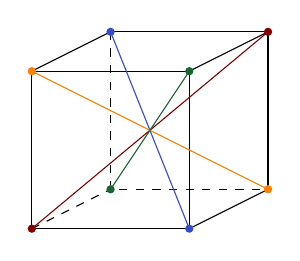
\begin{tikzpicture}
      \draw (0, 0) rectangle (2, 2);
      \draw (2, 0) -- +(1, 0.5);
      \draw (2, 2) -- +(1, 0.5);
      \draw (0, 2) -- +(1, 0.5);
      \draw [dashed] (0, 0) -- +(1, 0.5);
      \draw (1, 2.5) -- (3, 2.5) -- (3, 0.5);
      \draw [dashed] (1, 2.5) -- (1, 0.5) -- (3, 0.5);

      \draw [mred] (0, 0) node [circ] {} -- (3, 2.5) node [circ] {};
      \draw [mblue] (2, 0) node [circ] {} -- (1, 2.5) node [circ] {};
      \draw [morange] (0, 2) node [circ] {} -- (3, 0.5) node [circ] {};
      \draw [mgreen] (2, 2) node [circ] {} -- (1, 0.5) node [circ] {};
    \end{tikzpicture}
  \end{center}
  Then $G$ acts on $X$, and so we get $\phi: G \to \Sym(X)$. What is its kernel? To preserve the diagonals, it either does nothing to the diagonal, or flips the two vertices. So $G_X = \ker(\phi) = \{\id, \text{symmetry that sends each vertex to its opposite}\} \cong C_2$.

  How about the image? We have $G^X = \im(\phi) \leq \Sym(X) \cong S_4$. It is an exercise to show that $\im(\phi) = \Sym(X)$, i.e.\ that $\phi$ is surjective. We are not proving this because this is an exercise in geometry, not group theory. Then the first isomorphism theorem tells us
  \[
    G^X \cong G/G_X.
  \]
  So
  \[
    |G| = |G^X| |G_X| = 4! \cdot 2 = 48.
  \]
\end{eg}
This is an example of how we can use group actions to count elements in a group.

\begin{eg}[Cayley's theorem]\index{Cayley's theorem}
  For any group $G$, we have an action of $G$ on $G$ itself via
  \[
    g * g_1 = gg_1.
  \]
  It is trivial to check this is indeed an action. This gives a group homomorphism $\phi: G \to \Sym(G)$. What is its kernel? If $g \in \ker(\phi)$, then it acts trivially on every element. In particular, it acts trivially on the identity. So $g* e = e$, which means $g = e$. So $\ker(\phi) = \{e\}$. By the first isomorphism theorem, we get
  \[
    G \cong G/\{e\} \cong \im \phi \leq \Sym(G).
  \]
  So we know every group is (isomorphic to) a subgroup of a symmetric group.
\end{eg}

\begin{eg}
  Let $H$ be a subgroup of $G$, and $X = G/H$ be the set of left cosets of $H$. We let $G$ act on $X$ via
  \[
    g* g_1 H = gg_1 H.
  \]
  It is easy to check this is well-defined and is indeed a group action. So we get $\phi: G \to \Sym(X)$.

  Now consider $G_X = \ker(\phi)$. If $g \in G_X$, then for every $g_1 \in G$, we have $g * g_1 H = g_1H$. This means $g_1^{-1} gg_1 \in H$. In other words, we have
  \[
    g \in g_1 H g_1^{-1}.
  \]
  This has to happen for \emph{all} $g_1 \in G$. So
  \[
    G_X \subseteq \bigcap_{g_1 \in G} g_1 Hg_1^{-1}.
  \]
  This argument is completely reversible --- if $g \in \bigcap_{g_1 \in G} g_1 Hg_1^{-1}$, then for each $g_1 \in G$, we know
  \[
    g_1^{-1}g g_1 \in H,
  \]
  and hence
  \[
    gg_1 H = g_1H.
  \]
  So
  \[
    g* g_1 H = g_1 H
  \]
  So $g \in G_X$. Hence we indeed have equality:
  \[
    \ker (\phi) = G_X = \bigcap_{g_1 \in G} g_1 Hg_1^{-1}.
  \]
  Since this is a kernel, this is a normal subgroup of $G$, and is contained in $H$. Starting with an arbitrary subgroup $H$, this allows us to generate a normal subgroup, and this is indeed the biggest normal subgroup of $G$ that is contained in $H$, if we stare at it long enough.
\end{eg}

We can use this to prove the following theorem.
\begin{thm}
  Let $G$ be a finite group, and $H \leq G$ a subgroup of index $n$. Then there is a normal subgroup $K \lhd G$ with $K \leq H$ such that $G/K$ is isomorphic to a subgroup of $S_n$. Hence $|G/K| \mid n!$ and $|G/K| \geq n$.
\end{thm}

\begin{proof}
  We apply the previous example, giving $\phi: G \to \Sym(G/H)$, and let $K$ be the kernel of this homomorphism. We have already shown that $K \leq H$. Then the first isomorphism theorem gives
  \[
    G/K \cong \im \phi \leq \Sym(G/H) \cong S_n.
  \]
  Then by Lagrange's theorem, we know $|G/K| \mid |S_n| = n!$, and we also have $|G/K| \geq |G/H| = n$.
\end{proof}

\begin{cor}
  Let $G$ be a non-abelian simple group. Let $H \leq G$ be a proper subgroup of index $n$. Then $G$ is isomorphic to a subgroup of $A_n$. Moreover, we must have $n \geq 5$, i.e.\ $G$ cannot have a subgroup of index less than $5$.
\end{cor}

\begin{proof}
  The action of $G$ on $X = G/H$ gives a homomorphism $\phi: G \to \Sym(X)$. Then $\ker(\phi) \lhd G$. Since $G$ is simple, $\ker(\phi)$ is either $G$ or $\{e\}$. We first show that it cannot be $G$. If $\ker(\phi) = G$, then every element of $G$ acts trivially on $X = G/H$. But if $g \in G\setminus H$, which exists since the index of $H$ is not $1$, then $g * H = gH \not= H$. So $g$ does not act trivially. So the kernel cannot be the whole of $G$. Hence $\ker(\phi) = \{e\}$.

  Thus by the first isomorphism theorem, we get
  \[
    G \cong \im (\phi) \leq \Sym(X) \cong S_n.
  \]
  We now need to show that $G$ is in fact a subgroup of $A_n$.

  We know $A_n \lhd S_n$. So $\im(\phi) \cap A_n \lhd \im(\phi) \cong G$. As $G$ is simple, $\im (\phi) \cap A_n$ is either $\{e\}$ or $G = \im(\phi)$. We want to show that the second thing happens, i.e.\ the intersection is not the trivial group. We use the second isomorphism theorem. If $\im(\phi) \cap A_n = \{e\}$, then
  \[
    \im(\phi) \cong \frac{\im(\phi)}{\im(\phi) \cap A_n} \cong \frac{\im (\phi) A_n}{A_n} \leq \frac{S_n}{A_n} \cong C_2.
  \]
  So $G \cong \im (\phi)$ is a subgroup of $C_2$, i.e.\ either $\{e\}$ or $C_2$ itself. Neither of these are non-abelian. So this cannot be the case. So we must have $\im(\phi) \cap A_n = \im(\phi)$, i.e.\ $\im (\phi) \leq A_n$.

  The last part follows from the fact that $S_1, S_2, S_3, S_4$ have no non-abelian simple subgroups, which you can check by going to a quiet room and listing out all their subgroups.
\end{proof}

Let's recall some old definitions from IA Groups.
\begin{defi}[Orbit]\index{orbit}
  If $G$ acts on a set $X$, the \emph{orbit} of $x \in X$ is
  \[
    G\cdot x = \{g * x \in X: g \in G\}.
  \]
\end{defi}

\begin{defi}[Stabilizer]\index{stabilizer}
  If $G$ acts on a set $X$, the \emph{stabilizer} of $x \in X$ is
  \[
    G_x = \{g \in G: g * x = x\}.
  \]
\end{defi}

The main theorem about these concepts is the orbit-stabilizer theorem.
\begin{thm}[Orbit-stabilizer theorem]\index{orbit-stabilizer theorem}
  Let $G$ act on $X$. Then for any $x \in X$, there is a bijection between $G\cdot x$ and $G/G_x$, given by $g \cdot x \leftrightarrow g\cdot G_x$.

  In particular, if $G$ is finite, it follows that
  \[
    |G| = |G_x| |G \cdot x|.
  \]
\end{thm}
It takes some work to show this is well-defined and a bijection, but you've done it in IA Groups. In IA Groups, you probably learnt the second statement instead, but this result is more generally true for infinite groups.

\subsection{Conjugacy, centralizers and normalizers}
We have seen that every group acts on itself by multiplying on the left. A group $G$ can also act on itself in a different way, by conjugation:\index{conjugation}
\[
  g * g_1 = g g_1 g^{-1}.
\]
Let $\phi: G \to \Sym(G)$ be the associated permutation representation. We know, by definition, that $\phi(g)$ is a bijection from $G$ to $G$ as sets. However, here $G$ is not an arbitrary set, but is a group. A natural question to ask is whether $\phi(g)$ is a homomorphism or not. Indeed, we have
\[
  \phi(g) (g_1 \cdot g_2) = g g_1 g_2 g^{-1} = (g g_1 g^{-1})(g g_2 g^{-1}) = \phi(g)(g_1) \phi(g) (g_2).
\]
So $\phi(g)$ is a homomorphism from $G$ to $G$. Since $\phi(g)$ is bijective (as in \emph{any} group action), it is in fact an isomorphism.

Thus, for any group $G$, there are many isomorphisms from $G$ to itself, one for every $g \in G$, and can be obtained from a group action of $G$ on itself.

We can, of course, take the collection of all isomorphisms of $G$, and form a new group out of it.
\begin{defi}[Automorphism group]\index{automorphism group}
  The \emph{automorphism group} of $G$ is
  \[
    \Aut(G) = \{f: G \to G: f\text{ is a group isomorphism}\}.
  \]
  This is a group under composition, with the identity map as the identity.
\end{defi}
This is a subgroup of $\Sym(G)$, and the homomorphism $\phi: G\to \Sym(G)$ by conjugation lands in $\Aut(G)$.

This is pretty fun --- we can use this to cook up some more groups, by taking a group and looking at its automorphism group.

We can also take a group, take its automorphism group, and then take its automorphism group again, and do it again, and see if this process stabilizes, or becomes periodic, or something. This is left as an exercise for the reader.

\begin{defi}[Conjugacy class]\index{conjugacy class}
  The \emph{conjugacy class} of $g \in G$ is
  \[
    \ccl_G(g) = \{hgh^{-1}: h \in G\},
  \]
  i.e.\ the orbit of $g \in G$ under the conjugation action.
\end{defi}

\begin{defi}[Centralizer]\index{centralizer}
  The \emph{centralizer} of $g \in G$ is
  \[
    C_G(g) = \{h \in G: hgh^{-1} = g\},
  \]
  i.e.\ the stabilizer of $g$ under the conjugation action. This is alternatively the set of all $h \in G$ that commute with $g$.
\end{defi}

\begin{defi}[Center]\index{center}
  The \emph{center} of a group $G$ is
  \[
    Z(G) = \{h \in G: hg h^{-1} = g\text{ for all }g \in G\} = \bigcap_{g \in G} C_G(g) = \ker (\phi).
  \]
\end{defi}
These are the elements of the group that commute with everything else.

By the orbit-stabilizer theorem, for each $x \in G$, we obtain a bijection $\ccl(x) \leftrightarrow G/C_G(x)$.
\begin{prop}
  Let $G$ be a finite group. Then
  \[
    |\ccl(x)| = |G:C_G(x)| = |G|/|C_G(x)|.
  \]
\end{prop}
In particular, the size of each conjugacy class divides the order of the group.

Another useful notion is the normalizer.
\begin{defi}[Normalizer]\index{normalizer}
  Let $H \leq G$. The \emph{normalizer} of $H$ in $G$ is
  \[
    N_G(H) = \{g \in G: g^{-1}H g = H\}.
  \]
\end{defi}
Note that we certainly have $H \leq N_G(H)$. Even better, $H \lhd N_G(H)$, essentially by definition. This is in fact the biggest subgroup of $G$ in which $H$ is normal.

We are now going to look at conjugacy classes of $S_n$. Now we recall from IA Groups that permutations in $S_n$ are conjugate if and only if they have the same cycle type when written as a product of disjoint cycles. We can think of the cycle types as partitions of $n$. For example, the partition $2, 2, 1$ of $5$ corresponds to the conjugacy class of $(1\; 2)(3\; 4)(5)$. So the conjugacy classes of $S_n$ are exactly the partitions of $n$.

We will use this fact in the proof of the following theorem:
\begin{thm}
  The alternating groups $A_n$ are simple for $n \geq 5$ (also for $n = 1, 2, 3$).
\end{thm}
The cases in brackets follow from a direct check since $A_1 \cong A_2 \cong \{e\}$ and $A_3 \cong C_3$, all of which are simple. We can also check manually that $A_4$ has non-trivial normal subgroups, and hence not simple.

Recall we also proved that $A_5$ is simple in IA Groups by brute force --- we listed all its conjugacy classes, and see they cannot be put together to make a normal subgroup. This obviously cannot be easily generalized to higher values of $n$. Hence we need to prove this with a different approach.

\begin{proof}
  We start with the following claim:
  \begin{claim}
    $A_n$ is generated by $3$-cycles.
  \end{claim}
  As any element of $A_n$ is a product of evenly-many transpositions, it suffices to show that every product of two transpositions is also a product of $3$-cycles.

  There are three possible cases: let $a, b, c, d$ be distinct. Then
  \begin{enumerate}
    \item $(a\; b)(a\; b) = e$.
    \item $(a\; b)(b\; c) = (a\; b\; c)$.
    \item $(a\; b)(c\; d) = (a\; c\; b)(a\; c\; d)$.
  \end{enumerate}
  So we have shown that every possible product of two transpositions is a product of three-cycles.

  \begin{claim}
    Let $H \lhd A_n$. If $H$ contains a $3$-cycle, then we $H = A_n$.
  \end{claim}
  We show that if $H$ contains a $3$-cycle, then \emph{every} $3$-cycle is in $H$. Then we are done since $A_n$ is generated by $3$-cycles. For concreteness, suppose we know $(a\; b\; c) \in H$, and we want to show $(1\; 2\; 3) \in H$.

  Since they have the same cycle type, so we have $\sigma \in S_n$ such that $(a\; b\; c) = \sigma(1\; 2\; 3) \sigma^{-1}$. If $\sigma$ is even, i.e.\ $\sigma \in A_n$, then we have that $(1\; 2\; 3) \in \sigma^{-1}H\sigma = H$, by the normality of $H$ and we are trivially done.

  If $\sigma$ is odd, replace it by $\bar{\sigma} = \sigma \cdot (4\; 5)$. Here is where we use the fact that $n \geq 5$ (we will use it again later). Then we have
  \[
    \bar{\sigma} (1\; 2\; 3) \bar{\sigma}^{-1} = \sigma (4\; 5)(1\; 2\; 3)(4\; 5) \sigma^{-1} = \sigma(1\; 2\; 3) \sigma^{-1} = (a\; b\; c),
  \]
  using the fact that $(1\; 2\; 3)$ and $(4\; 5)$ commute. Now $\bar{\sigma}$ is even. So $(1\; 2\; 3) \in H$ as above.

  What we've got so far is that if $H \lhd A_n$ contains \emph{any} $3$-cycle, then it is $A_n$. Finally, we have to show that every normal subgroup must contain at least one $3$-cycle.
  \begin{claim}
    Let $H \lhd A_n$ be non-trivial. Then $H$ contains a $3$-cycle.
  \end{claim}
  We separate this into many cases
  \begin{enumerate}
    \item Suppose $H$ contains an element which can be written in disjoint cycle notation
      \[
        \sigma = (1\; 2\; 3 \cdots r) \tau,
      \]
      for $r \geq 4$. We now let $\delta = (1\; 2\; 3) \in A_n$. Then by normality of $H$, we know $\delta^{-1} \sigma \delta \in H$. Then $\sigma^{-1}\delta^{-1}\sigma \delta \in H$. Also, we notice that $\tau$ does not contain $1, 2, 3$. So it commutes with $\delta$, and also trivially with $(1\; 2\; 3\; \cdots\; r)$. We can expand this mess to obtain
      \[
        \sigma^{-1} \delta^{-1} \sigma\delta = (r\; \cdots \; 2\; 1)(1\; 3\; 2)(1\; 2\; 3\; \cdots \; r)(1\; 2\; 3) = (2\; 3 \; r),
      \]
      which is a $3$-cycle. So done.

      The same argument goes through if $\sigma = (a_1 \; a_2 \; \cdots \; a_r) \tau$ for any $a_1, \cdots, a_n$.
    \item Suppose $H$ contains an element consisting of at least two $3$-cycles in disjoint cycle notation, say
      \[
        \sigma = (1\; 2\; 3)(4\; 5\; 6)\tau
      \]
      We now let $\delta = (1\; 2\; 4)$, and again calculate
      \[
        \sigma^{-1} \delta^{-1}\sigma\delta = (1\; 3\; 2)(4\; 6\; 5)(1\; 4\; 2)(1\; 2\; 3)(4\; 5\; 6)(1\; 2\; 4) = (1\; 2\; 4\; 3\; 6).
      \]
      This is a $5$-cycle, which is necessarily in $H$. By the previous case, we get a $3$-cycle in $H$ too, and hence $H = A_n$.
    \item Suppose $H$ contains $\sigma = (1\; 2\; 3)\tau$, with $\tau$ a product of $2$-cycles (if $\tau$ contains anything longer, then it would fit in one of the previous two cases). Then $\sigma^2 = (1\; 2\; 3)^2 = (1\; 3\; 2)$ is a three-cycle.
    \item Suppose $H$ contains $\sigma = (1\; 2)(3\; 4)\tau$, where $\tau$ is a product of $2$-cycles. We first let $\delta = (1\; 2\; 3)$ and calculate
      \[
        u = \sigma^{-1}\delta^{-1}\sigma\delta = (1\; 2)(3\; 4)(1\; 3\; 2)(1\; 2)(3\; 4)(1\; 2\; 3) = (1\; 4)(2\; 3),
      \]
      which is again in $u$. We landed in the same case, but instead of two transpositions times a mess, we just have two transpositions, which is nicer. Now let
      \[
        v = (1\; 5\; 2)u (1\; 2\; 5) = (1\; 3)(4\; 5) \in H.
      \]
      Note that we used $n \geq 5$ again. We have yet again landed in the same case. Notice however, that these are not the same transpositions. We multiply
      \[
        uv = (1\; 4)(2\; 3)(1\; 3)(4\; 5) = (1\; 2\; 3\; 4\; 5) \in H.
      \]
      This is then covered by the first case, and we are done.
  \end{enumerate}
  So done. Phew.
\end{proof}

\subsection{Finite \texorpdfstring{$p$}{p}-groups}
Note that when studying the orders of groups and subgroups, we always talk about divisibility, since that is what Lagrange's theorem tells us about. We never talk about things like the sum of the orders of two subgroups. When it comes to divisibility, the simplest case would be when the order is a prime, and we have done that already. The next best thing we can hope for is that the order is a power of a prime.

\begin{defi}[$p$-group]\index{$p$-group}
  A finite group $G$ is a \emph{$p$-group} if $|G| = p^n$ for some prime number $p$ and $n \geq 1$.
\end{defi}

\begin{thm}
  If $G$ is a finite $p$-group, then $Z(G) = \{x \in G: xg = gx\text{ for all }g \in G\}$ is non-trivial.
\end{thm}
This immediately tells us that for $n \geq 2$, a $p$ group is never simple.

\begin{proof}
  Let $G$ act on itself by conjugation. The orbits of this action (i.e.\ the conjugacy classes) have order dividing $|G| = p^n$. So it is either a singleton, or its size is divisible by $p$.

  Since the conjugacy classes partition $G$, we know the total size of the conjugacy classes is $|G|$. In particular,
  \begin{multline*}
    |G| = \text{number of conjugacy class of size 1} \\
    + \sum \text{order of all other conjugacy classes}.
  \end{multline*}
  We know the second term is divisible by $p$. Also $|G| = p^n$ is divisible by $p$. Hence the number of conjugacy classes of size $1$ is divisible by $p$. We know $\{e\}$ is a conjugacy class of size $1$. So there must be at least $p$ conjugacy classes of size $1$. Since the smallest prime number is $2$, there is a conjugacy class $\{x\} \not= \{e\}$.

  But if $\{x\}$ is a conjugacy class on its own, then by definition $g^{-1}xg = x$ for all $g \in G$, i.e.\ $xg = gx$ for all $g \in G$. So $x \in Z(G)$. So $Z(G)$ is non-trivial.
\end{proof}
The theorem allows us to prove interesting things about $p$-groups by induction --- we can quotient $G$ by $Z(G)$, and get a smaller $p$-group. One way to do this is via the below lemma.

\begin{lemma}
  For any group $G$, if $G/Z(G)$ is cyclic, then $G$ is abelian.

  In other words, if $G/Z(G)$ is cyclic, then it is in fact trivial, since the center of an abelian group is the abelian group itself.
\end{lemma}

\begin{proof}
  Let $g \in Z(G)$ be a generator of the cyclic group $G/Z(G)$. Hence every coset of $Z(G)$ is of the form $g^rZ(G)$. So every element $x \in G$ must be of the form $g^r z$ for $z \in Z(G)$ and $r \in \Z$. To show $G$ is abelian, let $\bar{x} = g^{\bar{r}} \bar{z}$ be another element, with $\bar{z} \in Z(G), \bar{r} \in \Z$. Note that $z$ and $\bar{z}$ are in the center, and hence commute with every element. So we have
  \[
    x\bar{x} = g^r z g^{\bar{r}} \bar{z} = g^r g^{\bar{r}} z \bar{z} = g^{\bar{r}}g^r \bar{z} z = g^{\bar{r}}\bar{z} g^r z = \bar{x} x.
  \]
  So they commute. So $G$ is abelian.
\end{proof}

This is a general lemma for groups, but is particularly useful when applied to $p$ groups.
\begin{cor}
  If $p$ is prime and $|G| = p^2$, then $G$ is abelian.
\end{cor}

\begin{proof}
  Since $Z(G) \leq G$, its order must be $1$, $p$ or $p^2$. Since it is not trivial, it can only be $p$ or $p^2$. If it has order $p^2$, then it is the whole group and the group is abelian. Otherwise, $G/Z(G)$ has order $p^2/p = p$. But then it must be cyclic, and thus $G$ must be abelian. This is a contradiction. So $G$ is abelian.
\end{proof}

\begin{thm}
  Let $G$ be a group of order $p^a$, where $p$ is a prime number. Then it has a subgroup of order $p^b$ for any $0 \leq b \leq a$.
\end{thm}
This means there is a subgroup of every conceivable order. This is not true for general groups. For example, $A_5$ has no subgroup of order $30$ or else that would be a normal subgroup.

\begin{proof}
  We induct on $a$. If $a = 1$, then $\{e\}, G$ give subgroups of order $p^0$ and $p^1$. So done.

  Now suppose $a > 1$, and we want to construct a subgroup of order $p^b$. If $b = 0$, then this is trivial, namely $\{e\} \leq G$ has order $1$.

  Otherwise, we know $Z(G)$ is non-trivial. So let $x \not= e \in Z(G)$. Since $\ord(x) \mid |G|$, its order is a power of $p$. If it in fact has order $p^c$, then $x^{p^{c - 1}}$ has order $p$. So we can suppose, by renaming, that $x$ has order $p$. We have thus generated a subgroup $\bra x\ket$ of order exactly $p$. Moreover, since $x$ is in the center, $\bra x\ket$ commutes with everything in $G$. So $\bra x\ket$ is in fact a normal subgroup of $G$. This is the point of choosing it in the center. Therefore $G/\bra x\ket$ has order $p^{a - 1}$.

  Since this is a strictly smaller group, we can by induction suppose $G/\bra x\ket$ has a subgroup of any order. In particular, it has a subgroup $L$ of order $p^{b - 1}$. By the subgroup correspondence, there is some $K \leq G$ such that $L = K / \bra x\ket$ and $H \lhd K$. But then $K$ has order $p^b$. So done.
\end{proof}

\subsection{Finite abelian groups}
We now move on to a small section, which is small because we will come back to it later, and actually prove what we claim.

It turns out finite abelian groups are very easy to classify. We can just write down a list of all finite abelian groups. We write down the classification theorem, and then prove it in the last part of the course, where we hit this with a huge sledgehammer.

\begin{thm}[Classification of finite abelian groups]\index{classification of finite abelian groups}
  Let $G$ be a finite abelian group. Then there exist some $d_1, \cdots, d_r$ such that
  \[
    G \cong C_{d_1} \times C_{d_2} \times \cdots \times C_{d_r}.
  \]
  Moreover, we can pick $d_i$ such that $d_{i + 1} \mid d_i$ for each $i$, and this expression is unique.
\end{thm}
It turns out the best way to prove this is not to think of it as a group, but as a $\Z$-module, which is something we will come to later.

\begin{eg}
  The abelian groups of order $8$ are $C_8$, $C_4 \times C_2$, $C_2 \times C_2 \times C_2$.
\end{eg}

Sometimes this is not the most useful form of decomposition. To get a nicer decomposition, we use the following lemma:
\begin{lemma}
  If $n$ and $m$ are coprime, then $C_{mn} \cong C_m \times C_n$.
\end{lemma}
This is a grown-up version of the Chinese remainder theorem. This is what the Chinese remainder theorem really says.

\begin{proof}
  It suffices to find an element of order $nm$ in $C_m \times C_n$. Then since $C_n \times C_m$ has order $nm$, it must be cyclic, and hence isomorphic to $C_{nm}$.

  Let $g \in C_m$ have order $m$; $h \in C_n$ have order $n$, and consider $(g, h) \in C_m \times C_n$. Suppose the order of $(g, h)$ is $k$. Then $(g, h)^k = (e, e)$. Hence $(g^k, h^k) = (e, e)$. So the order of $g$ and $h$ divide $k$, i.e.\ $m \mid k$ and $n \mid k$. As $m$ and $n$ are coprime, this means that $mn \mid k$.

  As $k = \ord((g, h))$ and $(g, h) \in C_m \times C_n$ is a group of order $mn$, we must have $k \mid nm$. So $k = nm$.
\end{proof}

\begin{cor}
  For any finite abelian group $G$, we have
  \[
    G \cong C_{d_1} \times C_{d_2} \times \cdots \times C_{d_r},
  \]
  where each $d_i$ is some prime power.
\end{cor}

\begin{proof}
  From the classification theorem, iteratively apply the previous lemma to break each component up into products of prime powers.
\end{proof}

As promised, this is short.

\subsection{Sylow theorems}
We finally get to the big theorem of this part of the course.
\begin{thm}[Sylow theorems]\index{Sylow theorem}
  Let $G$ be a finite group of order $p^a \cdot m$, with $p$ a prime and $p \nmid m$. Then
  \begin{enumerate}
    \item The set of Sylow $p$-subgroups of $G$, given by
      \[
        \Syl_p(G) = \{P \leq G: |P| = p^a\},
      \]
      is non-empty. In other words, $G$ has a subgroup of order $p^a$.
    \item All elements of $\Syl_p(G)$ are conjugate in $G$.
    \item The number of Sylow $p$-subgroups $n_p = |\Syl_p(G)|$ satisfies $n_p \equiv 1 \pmod p$ and $n_p \mid |G|$ (in fact $n_p \mid m$, since $p$ is not a factor of $n_p$).
  \end{enumerate}
\end{thm}
These are sometimes known as Sylow's first/second/third theorem respectively.

We will not prove this just yet. We first look at how we can apply this theorem. We can use it without knowing how to prove it.

\begin{lemma}
  If $n_p = 1$, then the Sylow $p$-subgroup is normal in $G$.
\end{lemma}

\begin{proof}
  Let $P$ be the unique Sylow $p$-subgroup, and let $g \in G$, and consider $g^{-1}Pg$. Since this is isomorphic to $P$, we must have $|g^{-1} Pg| = p^a$, i.e.\ it is also a Sylow $p$-subgroup. Since there is only one, we must have $P = g^{-1}Pg$. So $P$ is normal.
\end{proof}

\begin{cor}
  Let $G$ be a non-abelian simple group. Then $|G| \mid \frac{n_p!}{2}$ for every prime $p$ such that $p \mid |G|$.
\end{cor}

\begin{proof}
  The group $G$ acts on $\Syl_p(G)$ by conjugation. So it gives a permutation representation $\phi: G \to \Sym(\Syl_p(G)) \cong S_{n_p}$. We know $\ker \phi \lhd G$. But $G$ is simple. So $\ker(\phi)= \{e\}$ or $G$. We want to show it is not the whole of $G$.

  If we had $G = \ker(\phi)$, then $g^{-1} Pg = P$ for all $g \in G$. Hence $P$ is a normal subgroup. As $G$ is simple, either $P = \{e\}$, or $P = G$. We know $P$ cannot be trivial since $p \mid |G|$. But if $G = P$, then $G$ is a $p$-group, has a non-trivial center, and hence $G$ is not non-abelian simple. So we must have $\ker(\phi) = \{e\}$.

  Then by the first isomorphism theorem, we know $G \cong \im \phi \leq S_{n_p}$. We have proved the theorem without the divide-by-two part. To prove the whole result, we need to show that in fact $\im (\phi) \leq A_{n_p}$. Consider the following composition of homomorphisms:
  \[
    \begin{tikzcd}
      G \ar[r, "\phi"] & S_{n_p} \ar[r, "\sgn"] & \{\pm 1\}.
    \end{tikzcd}
  \]
  If this is surjective, then $\ker (\sgn \circ \phi) \lhd G$ has index $2$ (since the index is the size of the image), and is not the whole of $G$. This means $G$ is not simple (the case where $|G| = C_2$ is ruled out since it is abelian).

  So the kernel must be the whole $G$, and $\sgn \circ \phi$ is the trivial map. In other words, $\sgn(\phi(g)) = +1$. So $\phi(g) \in A_{n_p}$. So in fact we have
  \[
    G \cong \im(\phi) \leq A_{n_p}.
  \]
  So we get $|G| \mid \frac{n_p!}{2}$.
\end{proof}

\begin{eg}
  Suppose $|G| = 1000$. Then $|G|$ is not simple. To show this, we need to factorize $1000$. We have $|G| = 2^3 \cdot 5^3$. We pick our favorite prime to be $p = 5$. We know $n_5 \cong 1 \pmod 5$, and $n_5 \mid 2^3 = 8$. The only number that satisfies this is $n_5 = 1$. So the Sylow $5$-subgroup is normal, and hence $G$ is not normal.
\end{eg}

\begin{eg}
  Let $|G| = 132 = 2^2 \cdot 3 \cdot 11$. We want to show this is not simple. So for a contradiction suppose it is.

  We start by looking at $p = 11$. We know $n_{11} \equiv 1 \pmod {11}$. Also $n_{11} \mid 12$. As $G$ is simple, we must have $n_{11} = 12$.

  Now look at $p = 3$. We have $n_3 = 1 \pmod 3$ and $n_3 \mid 44$. The possible values of $n_3$ are $4$ and $22$.

  If $n_3 = 4$, then the corollary says $|G| \mid \frac{4!}{2} = 12$, which is of course nonsense. So $n_3 = 22$.

  At this point, we count how many elements of each order there are. This is particularly useful if $p \mid |G|$ but $p^2 \nmid |G|$, i.e.\ the Sylow $p$-subgroups have order $p$ and hence are cyclic.

  As all Sylow $11$-subgroups are disjoint, apart from $\{e\}$, we know there are $12 \cdot (11 - 1) = 120$ elements of order $11$. We do the same thing with the Sylow $3$-subgroups. We need $22 \cdot (3 - 1) = 44$ elements of order $3$. But this is more elements than the group has. This can't happen. So $G$ must be simple.
\end{eg}

We now get to prove our big theorem. This involves some non-trivial amount of trickery.
\begin{proof}[Proof of Sylow's theorem]
  Let $G$ be a finite group with $|G| = p^a m$, and $p \nmid m$.
  \begin{enumerate}
    \item We need to show that $\Syl_p(G) \not= \emptyset$, i.e.\ we need to find some subgroup of order $p^a$. As always, we find something clever for $G$ to act on. We let
      \[
        \Omega = \{X\text{ sub\emph{set} of }G: |X| = p^a\}.
      \]
      We let $G$ act on $\Omega$ by
      \[
        g * \{g_1, g_2, \cdots, g_{p^a}\} = \{gg_1, gg_2, \cdots, gg_{p^a}\}.
      \]
      Let $\Sigma \leq \Omega$ be an orbit.

      We first note that if $\{g_1, \cdots, g_{p^a}\} \in \Sigma$, then by the definition of an orbit, for every $g \in G$,
      \[
        gg_1^{-1} * \{g_1, \cdots, g_{p^a}\} = \{g, gg_1^{-1}g_2, \cdots, gg_1^{-1} g_{p^a}\} \in \Sigma.
      \]
      The important thing is that this set contains $g$. So for each $g$, $\Sigma$ contains a set $X$ which contains $g$. Since each set $X$ has size $p^a$, we must have
      \[
        |\Sigma| \geq \frac{|G|}{p^a} = m.
      \]
      Suppose $|\Sigma| = m$. Then the orbit-stabilizer theorem says the stabilizer $H$ of any $\{g_1, \cdots, g_{p^a}\} \in \Sigma$ has index $m$, hence $|H| = p^a$, and thus $H \in \Syl_p(G)$.

      So we need to show that not every orbit $\Sigma$ can have size $> m$. Again, by the orbit-stabilizer, the size of any orbit divides the order of the group, $|G| = p^a m$. So if $|\Sigma| > m$, then $p \mid |\Sigma|$. Suppose we can show that $p \nmid |\Omega|$. Then not every orbit $\Sigma$ can have size $> m$, since $\Omega$ is the disjoint union of all the orbits, and thus we are done.

      So we have to show $p \nmid |\Omega|$. This is just some basic counting. We have
      \[
        |\Omega| = \binom{|G|}{p^a} = \binom{p^a m}{p^a} = \prod_{j = 0}^{p^a - 1} = \frac{p^a m - j}{p^a - j}.
      \]
      Now note that the largest power of $p$ dividing $p^am - j$ is the largest power of $p$ dividing $j$. Similarly, the largest power of $p$ dividing $p^a - j$ is also the largest power of $p$ dividing $j$. So we have the same power of $p$ on top and bottom for each item in the product, and they cancel. So the result is not divisible by $p$.

      This proof is not straightforward. We first needed the clever idea of letting $G$ act on $\Omega$. But then if we are given this set, the obvious thing to do would be to find something in $\Omega$ that is also a group. This is not what we do. Instead, we find an orbit whose stabilizer is a Sylow $p$-subgroup.

    \item We instead prove something stronger: if $Q \leq G$ is a $p$-subgroup (i.e.\ $|Q| = p^b$, for $b$ not necessarily $a$), and $P \leq G$ is a Sylow $p$-subgroup, then there is a $g \in G$ such that $g^{-1} Qg \leq P$. Applying this to the case where $Q$ is another Sylow $p$-subgroup says there is a $g$ such that $g^{-1}Qg \leq P$, but since $g^{-1}Qg$ has the same size as $P$, they must be equal.

      We let $Q$ act on the set of cosets of $G/P$ via
      \[
        q * gP = qgP.
      \]
      We know the orbits of this action have size dividing $|Q|$, so is either $1$ or divisible by $p$. But they can't all be divisible by $p$, since $|G/P|$ is coprime to $p$. So at least one of them have size $1$, say $\{gP\}$. In other words, for every $q \in Q$, we have $qgP = gP$. This means $g^{-1}qg \in P$. This holds for every element $q \in Q$. So we have found a $g$ such that $g^{-1}Qg \leq P$.

    \item Finally, we need to show that $n_p \cong 1 \pmod p$ and $n_p \mid |G|$, where $n_p = |\Syl_P(G)|$.

      The second part is easier --- by Sylow's second theorem, the action of $G$ on $\Syl_p(G)$ by conjugation has one orbit. By the orbit-stabilizer theorem, the size of the orbit, which is $|\Syl_p(G)| = n_p$, divides $|G|$. This proves the second part.

      For the first part, let $P \in \Syl_P(G)$. Consider the action by conjugation of $P$ on $\Syl_p(G)$. Again by the orbit-stabilizer theorem, the orbits each have size $1$ or size divisible by $p$. But we know there is one orbit of size $1$, namely $\{P\}$ itself. To show $n_p = |\Syl_P(G)| \cong 1\pmod p$, it is enough to show there are no other orbits of size $1$.

      Suppose $\{Q\}$ is an orbit of size $1$. This means for every $p \in P$, we get
      \[
        p^{-1} Qp = Q.
      \]
      In other words, $P \leq N_G(Q)$. Now $N_G(Q)$ is itself a group, and we can look at its Sylow $p$-subgroups. We know $Q \leq N_G(Q) \leq G$. So $p^a \mid |N_G(Q)| \mid p^a m$. So $p^a$ is the biggest power of $p$ that divides $|N_G(Q)|$. So $Q$ is a Sylow $p$-subgroup of $N_G(Q)$.

      Now we know $P \leq N_G(Q)$ is \emph{also} a Sylow $p$-subgroup of $N_G(Q)$. By Sylow's second theorem, they must be conjugate in $N_G(Q)$. But conjugating anything in $Q$ by something in $N_G(Q)$ does nothing, by definition of $N_G(Q)$. So we must have $P = Q$. So the only orbit of size $1$ is $\{P\}$ itself. So done.\qedhere
  \end{enumerate}
\end{proof}

This is all the theories of groups we've got. In the remaining time, we will look at some interesting examples of groups.
\begin{eg}
  Let $G = \GL_n(\Z/p)$, i.e.\ the set of invertible $n\times n$ matrices with entries in $\Z/p$, the integers modulo $p$. Here $p$ is obviously a prime. When we do rings later, we will study this properly.

  First of all, we would like to know the size of this group. A matrix $A \in \GL_n(\Z/p)$ is the same as $n$ linearly independent vectors in the vector space $(\Z/p)^n$. We can just work out how many there are. This is not too difficult, when you know how.

  We can pick the first vector, which can be anything except zero. So there are $p^n - 1$ ways of choosing the first vector. Next, we need to pick the second vector. This can be anything that is not in the span of the first vector, and this rules out $p$ possibilities. So there are $p^n - p$ ways of choosing the second vector. Continuing this chain of thought, we have
  \[
    |\GL_n(\Z/p)| = (p^n - 1)(p^n - p)(p^n - p^2) \cdots (p^n - p^{n - 1}).
  \]
  What is a Sylow $p$-subgroup of $\GL_n(\Z/p)$? We first work out what the order of this is. We can factorize that as
  \[
    |\GL_n(\Z/p)|= (1 \cdot p \cdot p^2 \cdot \cdots \cdot p^{n - 1}) ((p^n - 1)(p^{n - 1} - 1) \cdots (p - 1)).
  \]
  So the largest power of $p$ that divides $|\GL_n(\Z/p)|$ is $p^{\binom{n}{2}}$. Let's find a subgroup of size $p^{\binom{n}{2}}$. We consider matrices of the form
  \[
    U = \left\{
      \begin{pmatrix}
        1 & * & * & \cdots & *\\
        0 & 1 & * & \cdots & *\\
        0 & 0 & 1 & \cdots & *\\
        \vdots & \vdots & \vdots & \ddots & \vdots\\
        0 & 0 & 0 & \cdots & 1
      \end{pmatrix} \in \GL_n(\Z/p)
    \right\}.
  \]
  Then we know $|U| = p^{\binom{n}{2}}$ as each $*$ can be chosen to be anything in $\Z/p$, and there are $\binom{n}{2}$ $*$s.

  Is the Sylow $p$-subgroup unique? No. We can take the lower triangular matrices and get another Sylow $p$-subgroup.
\end{eg}

\begin{eg}
  Let's be less ambitious and consider $\GL_2(\Z/p)$. So
  \[
    |G| = p(p^2 - 1)(p - 1) = p(p - 1)^2 (p + 1).
  \]
  Let $\ell$ be another prime number such that $\ell \mid p - 1$. Suppose the largest power of $\ell$ that divides $|G|$ is $\ell^2$. Can we (explicitly) find a Sylow $\ell$-subgroup?

  First, we want to find an element of order $\ell$. How is $p - 1$ related to $p$ (apart from the obvious way)? We know that
  \[
    (\Z/p)^\times = \{x \in \Z/p:(\exists y)\, xy \equiv 1 \pmod p\} \cong C_{p - 1}.
  \]
  So as $\ell\mid p - 1$, there is a subgroup $C_\ell \leq C_{p - 1} \cong (\Z/p)^\times$. Then we immediately know where to find a subgroup of order $\ell^2$: we have
  \[
    C_\ell \times \C_\ell \leq (\Z/p)^* \times (\Z/p)^\times \leq \GL_2(\Z/p),
  \]
  where the final inclusion is the diagonal matrices, identifying
  \[
    (a, b) \leftrightarrow
    \begin{pmatrix}
      a & 0\\
      0 & b
    \end{pmatrix}.
  \]
  So this is the Sylow $\ell$-subgroup.
\end{eg}

\section{Rings}
\subsection{Definitions and examples}
We now move on to something completely different --- rings. In a ring, we are allowed to add, subtract, multiply but not divide. Our canonical example of a ring would be $\Z$, the integers, as studied in IA Numbers and Sets.

In this course, we are only going to consider rings in which multiplication is commutative, since these rings behave like ``number systems'', where we can study number theory. However, some of these rings do not behave like $\Z$. Thus one major goal of this part is to understand the different properties of $\Z$, whether they are present in arbitrary rings, and how different properties relate to one another.

\begin{defi}[Ring]\index{ring}
  A \emph{ring} is a quintuple $(R, +, \ph, 0_R, 1_R)$ where $0_R, 1_R \in R$, and $+, \ph: R \times R \to R$ are binary operations such that
  \begin{enumerate}
    \item $(R, +, 0_R)$ is an abelian group.
    \item The operation $\ph: R \times R \to R$ satisfies associativity, i.e.
      \[
        a\cdot (b\cdot c) = (a \cdot b)\cdot c,
      \]
      and identity:
      \[
        1_R \cdot r = r \cdot 1_R = r.
      \]
    \item Multiplication distributes over addition, i.e.
      \begin{align*}
        r_1 \cdot (r_2 + r_3) &= (r_1 \cdot r_2) + (r_1 \cdot r_3)\\
        (r_1 + r_2) \cdot r_3 &= (r_1 \cdot r_3) + (r_2 \cdot r_3).
      \end{align*}
  \end{enumerate}
\end{defi}

\begin{notation}
  If $R$ is a ring and $r \in R$, we write $-r$ for the inverse to $r$ in $(R, +, 0_R)$. This satisfies $r + (-r) = 0_R$. We write $r - s$ to mean $r + (-s)$ etc.
\end{notation}
Some people don't insist on the existence of the multiplicative identity, but we will for the purposes of this course.

Since we can add and multiply two elements, by induction, we can add and multiply any finite number of elements. However, the notions of infinite sum and product are undefined. It doesn't make sense to ask if an infinite sum converges.

\begin{defi}[Commutative ring]\index{commutative ring}
  We say a ring $R$ is \emph{commutative} if $a \cdot b = b \cdot a$ for all $a, b \in R$.
\end{defi}
From now onwards, all rings in this course are going to be commutative.

Just as we have groups and subgroups, we also have subrings.
\begin{defi}[Subring]\index{subring}
  Let $(R, +, \ph, 0_R, 1_R)$ be a ring, and $S \subseteq R$ be a subset. We say $S$ is a \emph{subring} of $R$ if $0_R, 1_R \in S$, and the operations $+, \ph$ make $S$ into a ring in its own right. In this case we write $S \leq R$.
\end{defi}

\begin{eg}
  The familiar number systems are all rings: we have $\Z \leq \Q \leq \R \leq \C$, under the usual $0, 1, +, \ph$.
\end{eg}

\begin{eg}
  The set $\Z[i] = \{a + ib: a, b \in \Z\} \leq \C$ is the \emph{Gaussian integers}, which is a ring.

  We also have the ring $\Q[\sqrt{2}] = \{a + b \sqrt{2} \in \R: a, b \in \Q\} \leq \R$.
\end{eg}
We will use the square brackets notation quite frequently. It should be clear what it should mean, and we will define it properly later.

In general, elements in a ring do not have inverses. This is not a bad thing. This is what makes rings interesting. For example, the division algorithm would be rather contentless if everything in $\Z$ had an inverse. Fortunately, $\Z$ only has two invertible elements --- $1$ and $-1$. We call these \emph{units}.

\begin{defi}[Unit]\index{unit}
  An element $u \in R$ is a \emph{unit} if there is another element $v \in R$ such that $u \cdot v = 1_R$.
\end{defi}
It is important that this depends on $R$, not just on $u$. For example, $2 \in \Z$ is not a unit, but $2 \in \Q$ is a unit (since $\frac{1}{2}$ is an inverse).

A special case is when (almost) everything is a unit.
\begin{defi}[Field]\index{field}
  A \emph{field} is a non-zero ring where every $u \not= 0_R \in R$ is a unit.
\end{defi}
We will later show that $0_R$ cannot be a unit except in a very degenerate case.

\begin{eg}
  $\Z$ is not a field, but $\Q, \R, \C$ are all fields.

  Similarly, $\Z[i]$ is not a field, while $\Q[\sqrt{2}]$ is.
\end{eg}

\begin{eg}
  Let $R$ be a ring. Then $0_R + 0_R = 0_R$, since this is true in the group $(R, +, 0_R)$. Then for any $r \in R$, we get
  \[
    r\cdot (0_R + 0_R) = r\cdot 0_R.
  \]
  We now use the fact that multiplication distributes over addition. So
  \[
    r \cdot 0_R + r \cdot 0_R = r \cdot 0_R.
  \]
  Adding $(-r \cdot 0_R)$ to both sides give
  \[
    r \cdot 0_R = 0_R.
  \]
  This is true for any element $r \in R$. From this, it follows that if $R \not= \{0\}$, then $1_R \not= 0_R$ --- if they were equal, then take $r \not= 0_R$. So
  \[
    r = r \cdot 1_R = r \cdot 0_R = 0_R,
  \]
  which is a contradiction.
\end{eg}
Note, however, that $\{0\}$ forms a ring (with the only possible operations and identities), the zero ring, albeit a boring one. However, this is often a counterexample to many things.

\begin{defi}[Product of rings]\index{product of rings}
  Let $R, S$ be rings. Then the \emph{product} $R \times S$ is a ring via
  \[
    (r, s) + (r', s') = (r + r', s + s'),\quad (r, s) \cdot (r', s') = (r\cdot r', s \cdot s').
  \]
  The zero is $(0_R, 0_S)$ and the one is $(1_R, 1_S)$.

  We can (but won't) check that these indeed are rings.
\end{defi}

\begin{defi}[Polynomial]\index{polynomial}
  Let $R$ be a ring. Then a \emph{polynomial} with coefficients in $R$ is an expression
  \[
    f = a_0 + a_1X + a_2 X^2 + \cdots + a_n X^n,
  \]
  with $a_i \in R$. The symbols $X^i$ are formal symbols.
\end{defi}
We identify $f$ and $f + 0_R \cdot X^{n + 1}$ as the same things.

\begin{defi}[Degree of polynomial]\index{degree}
  The \emph{degree} of a polynomial $f$ is the largest $m$ such that $a_m \not= 0$.
\end{defi}

\begin{defi}[Monic polynomial]\index{monic polynomial}
  Let $f$ have degree $m$. If $a_m = 1$, then $f$ is called \emph{monic}.
\end{defi}

\begin{defi}[Polynomial ring]\index{polynomial ring}
  We write $R[X]$ for the set of all polynomials with coefficients in $R$. The operations are performed in the obvious way, i.e.\ if $f = a_0 + a_1X + \cdots + A_n X^n$ and $g = b_0 + b_1X + \cdots + b_k X^k$ are polynomials, then
  \[
    f + g = \sum_{r = 0}^{\max\{n, k\}} (a_i + b_i) X^i,
  \]
  and
  \[
    f\cdot g = \sum_{i = 0}^{n + k} \left(\sum_{j = 0}^i a_j b_{i - j}\right) X^i,
  \]
  We identify $R$ with the constant polynomials, i.e.\ polynomials $\sum a_i X^i$ with $a_i = 0$ for $i > 0$. In particular, $0_R \in R$ and $1_R \in R$ are the zero and one of $R[X]$.
\end{defi}
This is in fact a ring.

Note that a polynomial is just a sequence of numbers, interpreted as the coefficients of some formal symbols. While it does indeed induce a function in the obvious way, we shall not identify the polynomial with the function given by it, since different polynomials can give rise to the same function.

For example, in $\Z/2\Z [X]$, $f = X^2 + X$ is not the zero polynomial, since its coefficients are not zero. However, $f(0) = 0$ and $f(1) = 0$. As a function, this is identically zero. So $f \not= 0$ as a polynomial but $f = 0$ as a function.

\begin{defi}[Power series]\index{power series}
  We write $R[[X]]$ for the ring of power series on $R$, i.e.
  \[
    f = a_0 + a_1 X + a_2 X^2 + \cdots,
  \]
  where each $a_i \in R$. This has addition and multiplication the same as for polynomials, but without upper limits.
\end{defi}
A power series is very much not a function. We don't talk about whether the sum converges or not, because it is not a sum.

\begin{eg}
  Is $1 - X \in R[X]$ a unit? For every $g = a_0 + \cdots + a_n X^n$ (with $a_n \not= 0$), we get
  \[
    (1 - X)g = \text{stuff} + \cdots - a_n X^{n + 1},
  \]
  which is not $1$. So $g$ cannot be the inverse of $(1 - X)$. So $(1 - X)$ is not a unit.

  However, $1 - X \in R[[X]]$ \emph{is} a unit, since
  \[
    (1 - X)(1 + X + X^2 + X^3 + \cdots) = 1.
  \]
\end{eg}

\begin{defi}[Laurent polynomials]\index{Laurent polynomial}
  The \emph{Laurent polynomials} on $R$ is the set $R[X, X^{-1}]$, i.e.\ each element is of the form
  \[
    f = \sum_{i \in \Z} a_i X^i
  \]
  where $a_i \in R$ and only finitely many $a_i$ are non-zero. The operations are the obvious ones.
\end{defi}
We can also think of Laurent series, but we have to be careful. We allow infinitely many positive coefficients, but only finitely many negative ones. Or else, in the formula for multiplication, we will have an infinite sum, which is undefined.

\begin{eg}
  Let $X$ be a set, and $R$ be a ring. Then the set of all functions on $X$, i.e.\ functions $f: X \to R$, is a ring with ring operations given by
  \[
    (f + g)(x) = f(x) + g(x),\quad (f\cdot g)(x) = f(x) \cdot g(x).
  \]
  Here zero is the constant function $0$ and one is the constant function $1$.

  Usually, we don't want to consider all functions $X \to R$. Instead, we look at some subrings of this. For example, we can consider the ring of all continuous functions $\R \to \R$. This contains, for example, the polynomial functions, which is just $\R[X]$ (since in $\R$, polynomials \emph{are} functions).
\end{eg}

\subsection{Homomorphisms, ideals, quotients and isomorphisms}
Just like groups, we will come up with analogues of homomorphisms, normal subgroups (which are now known as ideals), and quotients.

\begin{defi}[Homomorphism of rings]\index{homomorphism}
  Let $R, S$ be rings. A function $\phi: R \to S$ is a \emph{ring homomorphism} if it preserves everything we can think of, i.e.
  \begin{enumerate}
    \item $\phi(r_1 + r_2) = \phi(r_1) + \phi(r_2)$,
    \item $\phi(0_R) = 0_S$,
    \item $\phi(r_1 \cdot r_2) = \phi(r_1) \cdot \phi(r_2)$,
    \item $\phi(1_R) = 1_S$.
  \end{enumerate}
\end{defi}

\begin{defi}[Isomorphism of rings]\index{isomorphism}
  If a homomorphism $\phi: R \to S$ is a bijection, we call it an \emph{isomorphism}.
\end{defi}

\begin{defi}[Kernel]\index{kernel}
  The \emph{kernel} of a homomorphism $\phi: R \to S$ is
  \[
    \ker (\phi) = \{r \in R: \phi(r) = 0_S\}.
  \]
\end{defi}

\begin{defi}[Image]\index{image}
  The \emph{image} of $\phi: R \to S$ is
  \[
    \im(\phi) = \{s \in S: s = \phi(r) \text{ for some }r \in R\}.
  \]
\end{defi}

\begin{lemma}
  A homomorphism $\phi: R \to S$ is injective if and only if $\ker \phi = \{0_R\}$.
\end{lemma}

\begin{proof}
  A ring homomorphism is in particular a group homomorphism $\phi: (R, +, 0_R) \to (S, +, 0_S)$ of abelian groups. So this follows from the case of groups.
\end{proof}

In the group scenario, we had groups, subgroups and \emph{normal} subgroups, which are special subgroups. Here, we have a special kind of subsets of a ring that act like normal subgroups, known as \emph{ideals}.

\begin{defi}[Ideal]\index{ideal}
  A subset $I \subseteq R$ is an \emph{ideal}, written $I \lhd R$, if
  \begin{enumerate}
    \item It is an additive subgroup of $(R, +, 0_R)$, i.e.\ it is closed under addition and additive inverses.\hfill (additive closure)
    \item If $a \in I$ and $b \in R$, then $a \cdot b \in I$. \hfill (strong closure)
  \end{enumerate}
  We say $I$ is a proper ideal if $I \not= R$.
\end{defi}
Note that the multiplicative closure is stronger than what we require for subrings --- for subrings, it has to be closed under multiplication by its own elements; for ideals, it has to be closed under multiplication by everything in the world. This is similar to how normal subgroups not only have to be closed under internal multiplication, but also conjugation by external elements.

\begin{lemma}
  If $\phi: R \to S$ is a homomorphism, then $\ker(\phi)\lhd R$.
\end{lemma}

\begin{proof}
  Since $\phi: (R, +, 0_R) \to (S, +, 0_S)$ is a group homomorphism, the kernel is a subgroup of $(R, +, 0_R)$.

  For the second part, let $a \in \ker(\phi)$, $b \in R$. We need to show that their product is in the kernel. We have
  \[
    \phi(a\cdot b) = \phi(a) \cdot \phi(b) = 0 \cdot \phi(b) = 0.
  \]
  So $a \cdot b \in \ker(\phi)$.
\end{proof}

\begin{eg}
  Suppose $I \lhd R$ is an ideal, and $1_R \in I$. Then for any $r \in R$, the axioms entail $1_R \cdot r \in I$. But $1_R \cdot r = r$. So if $1_R \in I$, then $I = R$.

  In other words, every proper ideal does not contain $1$. In particular, every proper ideal is not a subring, since a subring must contain $1$.
\end{eg}
We are starting to diverge from groups. In groups, a normal subgroup is a subgroup, but here an ideal is not a subring.

\begin{eg}
  We can generalize the above a bit. Suppose $I \lhd R$ and $u \in I$ is a unit, i.e.\ there is some $v \in R$ such that $u \cdot v = 1_R$. Then by strong closure, $1_R = u \cdot v\in I$. So $I = R$.

  Hence proper ideals are not allowed to contain any unit at all, not just $1_R$.
\end{eg}

\begin{eg}
  Consider the ring $\Z$ of integers. Then every ideal of $\Z$ is of the form
  \[
    n\Z = \{\cdots, -2n, -n, 0, n, 2n, \cdots\} \subseteq \Z.
  \]
  It is easy to see this is indeed an ideal.

  To show these are all the ideals, let $I \lhd \Z$. If $I = \{0\}$, then $I = 0\Z$. Otherwise, let $n \in \N$ be the smallest positive element of $I$. We want to show in fact $I = n\Z$. Certainly $n\Z \subseteq I$ by strong closure.

  Now let $m \in I$. By the Euclidean algorithm, we can write
  \[
    m = q \cdot n + r
  \]
  with $0 \leq r < n$. Now $n,m \in I$. So by strong closure, $m, q \cdot n \in I$. So $r = m - q\cdot n \in I$. As $n$ is the smallest positive element of $I$, and $r < n$, we must have $r = 0$. So $m = q\cdot n \in n\Z$. So $I \subseteq n\Z$. So $I = n\Z$.
\end{eg}
The key to proving this was that we can perform the Euclidean algorithm on $\Z$. Thus, for any ring $R$ in which we can ``do Euclidean algorithm'', every ideal is of the form $aR = \{a \cdot r: r \in R\}$ for some $a \in R$. We will make this notion precise later.

\begin{defi}[Generator of ideal]\index{generator of ideal}
  For an element $a \in R$, we write
  \[
    (a) = aR = \{a \cdot r: r \in R\} \lhd R.
  \]
  This is the \emph{ideal generated by $a$}.

  In general, let $a_1, a_2, \cdots, a_k \in R$, we write
  \[
    (a_1, a_2, \cdots, a_k) = \{ a_1 r_1 + \cdots + a_k r_k : r_1, \cdots, r_k \in R\}.
  \]
  This is the \emph{ideal generated by $a_1, \cdots, a_k$}.
\end{defi}
We can also have ideals generated by infinitely many objects, but we have to be careful, since we cannot have infinite sums.
\begin{defi}[Generator of ideal]\index{generator of ideal}
  For $A \subseteq R$ a subset, the \emph{ideal generated by $A$} is
  \[
    (A) = \left\{\sum_{a \in A} r_a \cdot a: r_a \in R, \text{ only finitely-many non-zero}\right\}.
  \]
\end{defi}

These ideals are rather nice ideals, since they are easy to describe, and often have some nice properties.
\begin{defi}[Principal ideal]\index{principal ideal}
  An ideal $I$ is a \emph{principal ideal} if $I = (a)$ for some $a \in R$.
\end{defi}
So what we have just shown for $\Z$ is that all ideals are principal. Not all rings are like this. These are special types of rings, which we will study more in depth later.

\begin{eg}
  Consider the following subset:
  \[
    \{f \in \R[X]: \text{ the constant coefficient of }f \text{ is }0\}.
  \]
  This is an ideal, as we can check manually (alternatively, it is the kernel of the ``evaluate at $0$'' homomorphism). It turns out this is a principal ideal. In fact, it is $(X)$.
\end{eg}

We have said ideals are like normal subgroups. The key idea is that we can divide by ideals.

\begin{defi}[Quotient ring]\index{quotient ring}
  Let $I \lhd R$. The \emph{quotient ring} $R/I$ consists of the (additive) cosets $r + I$ with the zero and one as $0_R + I$ and $1_R + I$, and operations
  \begin{align*}
    (r_1 + I) + (r_2 + I) &= (r_1 + r_2) + I\\
    (r_1 + I) \cdot (r_2 + I) &= r_1r_2 + I.
  \end{align*}
\end{defi}

\begin{prop}
  The quotient ring is a ring, and the function
  \begin{align*}
    R &\to R/I\\
    r &\mapsto r + I
  \end{align*}
  is a ring homomorphism.
\end{prop}
This is true, because we defined ideals to be those things that can be quotiented by. So we just have to check we made the right definition.

Just as we could have come up with the definition of a normal subgroup by requiring operations on the cosets to be well-defined, we could have come up with the definition of an ideal by requiring the multiplication of cosets to be well-defined, and we would end up with the strong closure property.

\begin{proof}
  We know the group $(R/I, +, 0_{R/I})$ is well-defined, since $I$ is a (normal) subgroup of $R$. So we only have to check multiplication is well-defined.

  Suppose $r_1 + I = r_1' + I$ and $r_2 + I = r_2' + I$. Then $r_1' - r_1 = a_1 \in I$ and $r_2' - r_2 = a_2 \in I$. So
  \[
    r_1' r_2' = (r_1 + a_1) (r_2 + a_2) = r_1 r_2 + r_1a_2 + r_2a_1 + a_1a_2.
  \]
  By the strong closure property, the last three objects are in $I$. So $r_1' r_2' + I = r_1r_2 + I$.

  It is easy to check that $0_R + I$ and $1_R + I$ are indeed the zero and one, and the function given is clearly a homomorphism.
\end{proof}

\begin{eg}
  We have the ideals $n\Z \lhd \Z$. So we have the quotient rings $\Z / n\Z$. The elements are of the form $m + n\Z$, so they are just
  \[
    0 + n\Z, 1 + n\Z, 2 + n\Z, \cdots, (n - 1) + n\Z.
  \]
  Addition and multiplication are just what we are used to --- addition and multiplication modulo $n$.
\end{eg}

Note that it is easier to come up with ideals than normal subgroups --- we can just pick up random elements, and then take the ideal generated by them.
\begin{eg}
  Consider $(X) \lhd \C[X]$. What is $\C[X]/(X)$? Elements are represented by
  \[
    a_0 + a_1 X + a_2 X^2 + \cdots + a_n X^n + (X).
  \]
  But everything but the first term is in $(X)$. So every such thing is equivalent to $a_0 + (X)$. It is not hard to convince yourself that this representation is unique. So in fact $\C[X]/(X) \cong \C$, with the bijection $a_0 + (X) \leftrightarrow a_0$.
\end{eg}
If we want to prove things like this, we have to convince ourselves this representation is unique. We can do that by hand here, but in general, we want to be able to do this properly.

\begin{prop}[Euclidean algorithm for polynomials]\index{Euclidean algorithm for polynomials}
  Let $\F$ be a field and $f, g \in \F[X]$. Then there is some $r, q \in \F[X]$ such that
  \[
    f = gq + r,
  \]
  with $\deg r < \deg g$.
\end{prop}
This is like the usual Euclidean algorithm, except that instead of the absolute value, we use the degree to measure how ``big'' the polynomial is.

\begin{proof}
  Let $\deg (f) = n$. So
  \[
    f = \sum_{i = 0}^n a_i X^i,
  \]
  and $a_n \not= 0$. Similarly, if $\deg g = m$, then
  \[
    g = \sum_{i = 0}^m b_i X^i,
  \]
  with $b_m \not= 0$. If $n < m$, we let $q = 0$ and $r = f$, and done.

  Otherwise, suppose $n \geq m$, and proceed by induction on $n$.

  We let
  \[
    f_1 = f - a_n b_m^{-1} X^{n - m} g.
  \]
  This is possible since $b_m \not= 0$, and $\F$ is a field. Then by construction, the coefficients of $X^n$ cancel out. So $\deg (f_1) < n$.

  If $n = m$, then $\deg (f_1) < n = m$. So we can write
  \[
    f = (a_n b_m^{-1} X^{n - m})g + f_1,
  \]
  and $\deg(f_1) < \deg(f)$. So done. Otherwise, if $n > m$, then as $\deg(f_1) < n$, by induction, we can find $r_1, q_1$ such that
  \[
    f_1 = g q_1 + r_1,
  \]
  and $\deg (r_1) < \deg g = m$. Then
  \[
    f = a_nb_m^{-1} X^{n - m} g + q_1 g + r_1 = (a_n b_m^{-1}X^{n - m} + q_1) g + r_1.
  \]
  So done.
\end{proof}
Now that we have a Euclidean algorithm for polynomials, we should be able to show that every ideal of $\F[X]$ is generated by one polynomial. We will not prove it specifically here, but later show that in \emph{general}, in every ring where the Euclidean algorithm is possible, all ideals are principal.

We now look at some applications of the Euclidean algorithm.
\begin{eg}
  Consider $\R[X]$, and consider the principal ideal $(X^2 + 1) \lhd \R[X]$. We let $R = \R[X]/(X^2 + 1)$.

  Elements of $R$ are polynomials
  \[
    \underbrace{a_0 + a_1X + a_2 X^2 + \cdots + a_n X^n}_{f} + (X^2 + 1).
  \]
  By the Euclidean algorithm, we have
  \[
    f = q(X^2 + 1) + r,
  \]
  with $\deg(r) < 2$, i.e.\ $r = b_0 + b_1 X$. Thus $f + (X^2 + 1) = r + (X^2 + 1)$. So every element of $\R[X]/(X^2 + 1)$ is representable as $a + bX$ for some $a, b \in \R$.

  Is this representation unique? If $a + bX + (X^2 + 1) = a' + b' X + (X^2 + 1)$, then the difference $(a - a') + (b - b')X \in (X^2 + 1)$. So it is $(X^2 + 1)q$ for some $q$. This is possible only if $q = 0$, since for non-zero $q$, we know $(X^2 + 1)q$ has degree at least $2$. So we must have $(a - a') + (b - b')X = 0$. So $a + bX = a' + b'X$. So the representation is unique.

  What we've got is that every element in $R$ is of the form $a + bX$, and $X^2 + 1 = 0$, i.e.\ $X^2 = -1$. This sounds like the complex numbers, just that we are calling it $X$ instead of $i$.

  To show this formally, we define the function
  \begin{align*}
    \phi: \R[X]/(X^2 + 1) &\to \C\\
    a + bX + (X^2 + 1) & \mapsto a + bi.
  \end{align*}
  This is well-defined and a bijection. It is also clearly additive. So to prove this is an isomorphism, we have to show it is multiplicative. We check this manually. We have
  \begin{align*}
    &\phi((a + bX + (X^2 + 1))(c + dX + (X^2 + 1))) \\
    ={}& \phi(ac + (ad + bc)X + bdX^2 + (X^2 + 1))\\
    ={}& \phi((ac - bd) + (ad + bc)X + (X^2 + 1))\\
    ={}& (ac - bd) + (ad + bc)i\\
    ={}& (a + bi) (c + di)\\
    ={}& \phi(a + bX + (X^2 + 1))\phi(c + dX + (X^2 + 1)).
  \end{align*}
  So this is indeed an isomorphism.
\end{eg}

This is pretty tedious. Fortunately, we have some helpful results we can use, namely the isomorphism theorems. These are exactly analogous to those for groups.
\begin{thm}[First isomorphism theorem]\index{first isomorphism theorem}
  Let $\phi: R \to S$ be a ring homomorphism. Then $\ker (\phi) \lhd R$, and
  \[
    \frac{R}{\ker (\phi)} \cong \im(\phi) \leq S.
  \]
\end{thm}

\begin{proof}
  We have already seen $\ker(\phi) \lhd R$. Now define
  \begin{align*}
    \Phi: R/\ker(\phi) &\to \im(\phi)\\
    r + \ker(\phi) &\mapsto \phi(r).
  \end{align*}
  This well-defined, since if $r + \ker(\phi) = r' + \ker(\phi)$, then $r - r' \in \ker(\phi)$. So $\phi(r - r') = 0$. So $\phi(r) = \phi(r')$.

  We don't have to check this is bijective and additive, since that comes for free from the (proof of the) isomorphism theorem of groups. So we just have to check it is multiplicative. To show $\Phi$ is multiplicative, we have
  \begin{align*}
    \Phi((r + \ker(\phi))(t + \ker(\phi))) &= \Phi(rt + \ker(\phi)) \\
    &= \phi(rt) \\
    &= \phi(r)\phi(t) \\
    &= \Phi(r + \ker(\phi)) \Phi(t + \ker(\phi)).\qedhere
  \end{align*}
\end{proof}
This is more-or-less the same proof as the one for groups, just that we had a few more things to check.

Since there is the \emph{first} isomorphism theorem, we, obviously, have more coming.

\begin{thm}[Second isomorphism theorem]\index{second isomorphism theorem}
  Let $R \leq S$ and $J \lhd S$. Then $J \cap R \lhd R$, and
  \[
    \frac{R + J}{J} = \{r + J: r \in R\} \leq \frac{S}{J}
  \]
  is a subring, and
  \[
    \frac{R}{R \cap J} \cong \frac{R + J}{J}.
  \]
\end{thm}

\begin{proof}
  Define the function
  \begin{align*}
    \phi: R &\to S/J\\
    r &\mapsto r + J.
  \end{align*}
  Since this is the quotient map, it is a ring homomorphism. The kernel is
  \[
    \ker(\phi) = \{r \in R: r + J = 0,\text{ i.e.\ } r \in J\} = R \cap J.
  \]
  Then the image is
  \[
    \im(\phi) = \{r + J: r \in R\} = \frac{R + J}{J}.
  \]
  Then by the first isomorphism theorem, we know $R \cap J \lhd R$, and $\frac{R + J}{J} \leq S$, and
  \[
    \frac{R}{R \cap J} \cong \frac{R + J}{J}.\qedhere
  \]
\end{proof}

Before we get to the third isomorphism theorem, recall we had the subgroup correspondence for groups. Analogously, for $I \lhd R$,
\begin{align*}
  \{\text{subrings of }R/I\} &\longleftrightarrow\{\text{subrings of }R\text{ which contain }I\}\\
  L \leq \frac{R}{I} &\longrightarrow \{x \in R: x + I \in L\}\\
  \frac{S}{I} \leq \frac{R}{I} &\longleftarrow I \lhd S \leq R.
\end{align*}
This is exactly the same formula as for groups.

For groups, we had a correspondence for normal subgroups. Here, we have a correspondence between ideals
\[
  \{\text{ideals of }R/I\} \longleftrightarrow\{\text{ideals of }R\text{ which contain }I\}\\
\]
It is important to note here that quotienting in groups and rings have different purposes. In groups, we take quotients so that we have simpler groups to work with. In rings, we often take quotients to get more interesting rings. For example, $\R[X]$ is quite boring, but $\R[X]/(X^2 + 1) \cong \C$ is more interesting. Thus this ideal correspondence allows us to occasionally get interesting ideals from boring ones.

\begin{thm}[Third isomorphism theorem]\index{third isomorphism theorem}
  Let $I \lhd R$ and $J \lhd R$, and $I \subseteq J$. Then $J / I \lhd R/I$ and
  \[
    \left(\frac{R}{I}\right) \big/ \left(\frac{J}{I}\right) \cong \frac{R}{J}.
  \]
\end{thm}

\begin{proof}
  We define the map
  \begin{align*}
    \phi: R/I &\to R/J\\
    r + I &\mapsto r + J.
  \end{align*}
  This is well-defined and surjective by the groups case. Also it is a ring homomorphism since multiplication in $R/I$ and $R/J$ are ``the same''. The kernel is
  \[
    \ker(\phi) = \{r + I: r + J = 0,\text{ i.e.\ } r \in J\} = \frac{J}{I}.
  \]
  So the result follows from the first isomorphism theorem.
\end{proof}

Note that for any ring $R$, there is a unique ring homomorphism $\Z \to R$, given by
\begin{align*}
  \iota: \Z &\to R\\
  n \geq 0 &\mapsto \underbrace{1_R + 1_R + \cdots + 1_R}_{n\text{ times}}\\
  n \leq 0 &\mapsto -(\underbrace{1_R + 1_R + \cdots + 1_R}_{-n\text{ times}})
\end{align*}
Any homomorphism $\Z \to R$ must be given by this formula, since it must send the unit to the unit, and we can show this is indeed a homomorphism by distributivity. So the ring homomorphism is unique. In fancy language, we say $\Z$ is the initial object in (the category of) rings.

We then know $\ker(\iota) \lhd \Z$. Thus $\ker(\iota) = n\Z$ for some $n$.

\begin{defi}[Characteristic of ring]\index{characteristic}
  Let $R$ be a ring, and $\iota: \Z \to R$ be the unique such map. The \emph{characteristic} of $R$ is the unique non-negative $n$ such that $\ker (\iota) = n\Z$.
\end{defi}

\begin{eg}
  The rings $\Z, \Q, \R, \C$ all have characteristic $0$. The ring $\Z / n\Z$ has characteristic $n$. In particular, all natural numbers can be characteristics.
\end{eg}
The notion of the characteristic will not be too useful in this course. However, fields of non-zero characteristic often provide interesting examples and counterexamples to some later theory.

\subsection{Integral domains, field of factions, maximal and prime ideals}
Many rings can be completely nothing like $\Z$. For example, in $\Z$, we know that if $a, b \not= 0$, then $ab \not= 0$. However, in, say, $\Z/6\Z$, we get $2, 3 \not= 0$, but $2 \cdot 3 = 0$. Also, $\Z$ has some nice properties such as every ideal is principal, and every integer has an (essentially) unique factorization. We will now classify rings according to which properties they have.

We start with the most fundamental property that the product of two non-zero elements are non-zero. We will almost exclusively work with rings that satisfy this property.
\begin{defi}[Integral domain]\index{integral domain}
  A non-zero ring $R$ is an \emph{integral domain} if for all $a, b \in R$, if $a \cdot b = 0_R$, then $a = 0_R$ or $b = 0_R$.
\end{defi}

An element that violates this property is known as a \emph{zero divisor}.
\begin{defi}[Zero divisor]\index{zero divisor}
  An element $x \in R$ is a \emph{zero divisor} if $x \not = 0$ and there is a $y \not= 0$ such that $x \cdot y = 0 \in R$.
\end{defi}
In other words, a ring is an integral domain if it has no zero divisors.

\begin{eg}
  All fields are integral domains, since if $a \cdot b = 0$, and $b \not= 0$, then $a = a\cdot (b\cdot b^{-1}) = 0$. Similarly, if $a\not= 0$, then $b = 0$.
\end{eg}

\begin{eg}
  A subring of an integral domain is an integral domain, since a zero divisor in the small ring would also be a zero divisor in the big ring.
\end{eg}

\begin{eg}
  Immediately, we know $\Z, \Q, \R, \C$ are integral domains, since $\C$ is a field, and the others are subrings of it. Also, $\Z[i] \leq \C$ is also an integral domain.
\end{eg}
These are the nice rings we like in number theory, since there we can sensibly talk about things like factorization.

It turns out there are no interesting finite integral domains.
\begin{lemma}
  Let $R$ be a finite ring which is an integral domain. Then $R$ is a field.
\end{lemma}

\begin{proof}
  Let $a \in R$ be non-zero, and consider the ring homomorphism
  \begin{align*}
    a \cdot -: R &\to R\\
    b &\mapsto a \cdot b
  \end{align*}
  We want to show this is injective. For this, it suffices to show the kernel is trivial. If $r \in \ker (a \cdot -)$, then $a \cdot r = 0$. So $r = 0$ since $R$ is an integral domain. So the kernel is trivial.

  Since $R$ is finite, $a\cdot -$ must also be surjective. In particular, there is an element $b \in R$ such that $a \cdot b = 1_R$. So $a$ has an inverse. Since $a$ was arbitrary, $R$ is a field.
\end{proof}

So far, we know fields are integral domains, and subrings of integral domains are integral domains. We have another good source of integral domain as follows:
\begin{lemma}
  Let $R$ be an integral domain. Then $R[X]$ is also an integral domain.
\end{lemma}

\begin{proof}
  We need to show that the product of two non-zero elements is non-zero. Let $f, g\in R[X]$ be non-zero, say
  \begin{align*}
    f &= a_0 + a_1X + \cdots + a_n X^n \in R[X]\\
    g &= b_0 + b_1X + \cdots + b_m X^m \in R[X],
  \end{align*}
  with $a_n, b_m \not= 0$. Then the coefficient of $X^{n + m}$ in $fg$ is $a_n b_m$. This is non-zero since $R$ is an integral domain. So $fg$ is non-zero. So $R[X]$ is an integral domain.
\end{proof}
So, for instance, $\Z[X]$ is an integral domain.

We can also iterate this.

\begin{notation}
  Write $R[X, Y]$ for $(R[X])[Y]$, the polynomial ring of $R$ in two variables. In general, write $R[X_1, \cdots, X_n] = (\cdots((R[X_1])[X_2]) \cdots )[X_n]$.
\end{notation}

Then if $R$ is an integral domain, so is $R[X_1, \cdots, X_n]$.

We now mimic the familiar construction of $\Q$ from $\Z$. For any integral domain $R$, we want to construct a field $F$ that consists of ``fractions'' of elements in $R$. Recall that a subring of any field is an integral domain. This says the converse --- every integral domain is the subring of some field.

\begin{defi}[Field of fractions]\index{field of fractions}
  Let $R$ be an integral domain. A \emph{field of fractions} $F$ of $R$ is a field with the following properties
  \begin{enumerate}
    \item $R \leq F$
    \item Every element of $F$ may be written as $a \cdot b^{-1}$ for $a, b \in R$, where $b^{-1}$ means the multiplicative inverse to $b \not= 0$ in $F$.
  \end{enumerate}
\end{defi}
For example, $\Q$ is the field of fractions of $\Z$.

\begin{thm}
  Every integral domain has a field of fractions.
\end{thm}

\begin{proof}
  The construction is exactly how we construct the rationals from the integers --- as equivalence classes of pairs of integers. We let
  \[
    S = \{(a, b) \in R \times R: b \not= 0\}.
  \]
  We think of $(a, b) \in S$ as $\frac{a}{b}$. We define the equivalence relation $\sim$ on $S$ by
  \[
    (a, b) \sim (c, d) \Leftrightarrow ad = bc.
  \]
  We need to show this is indeed a equivalence relation. Symmetry and reflexivity are obvious. To show transitivity, suppose
  \[
    (a, b) \sim (c, d),\quad (c, d) \sim (e, f),
  \]
  i.e.
  \[
    ad = bc,\quad cf = de.
  \]
  We multiply the first equation by $f$ and the second by $b$, to obtain
  \[
    adf = bcf,\quad bcf = bed.
  \]
  Rearranging, we get
  \[
    d(af - be) = 0.
  \]
  Since $d$ is in the denominator, $d \not= 0$. Since $R$ is an integral domain, we must have $af - be = 0$, i.e.\ $af = be$. So $(a, b) \sim (e, f)$. This is where being an integral domain is important.

  Now let
  \[
    F = S/{\sim}
  \]
  be the set of equivalence classes. We now want to check this is indeed the field of fractions. We first want to show it is a field. We write $\frac{a}{b} = [(a, b)] \in F$, and define the operations by
  \begin{align*}
    \frac{a}{b} + \frac{c}{d} &= \frac{ad + bc}{bd}\\
    \frac{a}{b}\cdot \frac{c}{d} &= \frac{ac}{bd}.
  \end{align*}
  These \emph{are} well-defined, and make $(F, +, \cdot, \frac{0}{1}, \frac{1}{1})$ into a ring. There are many things to check, but those are straightforward, and we will not waste time doing that here.

  Finally, we need to show every non-zero element has an inverse. Let $\frac{a}{b} \not= 0_F$, i.e.\ $\frac{a}{b} \not= \frac{0}{1}$, or $a\cdot 1 \not= b \cdot 0 \in R$, i.e.\ $a \not= 0$. Then $\frac{b}{a} \in F$ is defined, and
  \[
    \frac{b}{a} \cdot \frac{a}{b} = \frac{ba}{ba} = 1_F.
  \]
  So $\frac{a}{b}$ has a multiplicative inverse. So $F$ is a field.

  We now need to construct a subring of $F$ that is isomorphic to $R$. To do so, we need to define an injective isomorphism $\phi: R \to F$. This is given by
  \begin{align*}
    \phi: R &\to F\\
    r &\mapsto \frac{r}{1}.
  \end{align*}
  This is a ring homomorphism, as one can check easily. The kernel is the set of all $r \in R$ such that $\frac{r}{1} = 0$, i.e.\ $r = 0$. So the kernel is trivial, and $\phi$ is injective. Then by the first isomorphism theorem, $R \cong \im(\phi) \subseteq F$.

  Finally, we need to show everything is a quotient of two things in $R$. We have
  \[
    \frac{a}{b} = \frac{a}{1} \cdot \frac{1}{b} = \frac{a}{1}\cdot \left(\frac{b}{1}\right)^{-1},
  \]
  as required.
\end{proof}
This gives us a very useful tool. Since this gives us a field from an integral domain, this allows us to use field techniques to study integral domains. Moreover, we can use this to construct new interesting fields from integral domains.

\begin{eg}
  Consider the integral domain $\C[X]$. Its field of fractions is the field of all rational functions $\frac{p(X)}{q(X)}$, where $p, q \in \C[X]$.
\end{eg}
To some people, it is a shame to think of rings as having elements. Instead, we should think of a ring as a god-like object, and the only things we should ever mention are its ideals. We should also not think of the ideals as containing elements, but just some abstract objects, and all we know is how ideals relate to one another, e.g.\ if one contains the other.

Under this philosophy, we can think of a field as follows:
\begin{lemma}
  A (non-zero) ring $R$ is a field if and only if its only ideals are $\{0\}$ and $R$.
\end{lemma}
Note that we don't need elements to define the ideals $\{0\}$ and $R$. $\{0\}$ can be defined as the ideal that all other ideals contain, and $R$ is the ideal that contains all other ideals. Alternatively, we can reword this as ``$R$ is a field if and only if it has only two ideals'' to avoid mentioning explicit ideals.

\begin{proof}
  $(\Rightarrow)$ Let $I \lhd R$ and $R$ be a field. Suppose $x \not= 0 \in I$. Then as $x$ is a unit, $I = R$.

  $(\Leftarrow)$ Suppose $x \not= 0 \in R$. Then $(x)$ is an ideal of $R$. It is not $\{0\}$ since it contains $x$. So $(x) = R$. In other words $1_R \in (x)$. But $(x)$ is defined to be $\{x \cdot y: y \in R\}$. So there is some $u \in R$ such that $x\cdot u = 1_R$. So $x$ is a unit. Since $x$ was arbitrary, $R$ is a field.
\end{proof}
This is another reason why fields are special. They have the simplest possible ideal structure.

This motivates the following definition:

\begin{defi}[Maximal ideal]\index{maximal ideal}
  An ideal $I$ of a ring $R$ is \emph{maximal} if $I \not= R$ and for any ideal $J$ with $I \leq J \leq R$, either $J = I$ or $J = R$.
\end{defi}

The relation with what we've done above is quite simple. There is an easy way to recognize if an ideal is maximal.

\begin{lemma}
  An ideal $I \lhd R$ is maximal if and only if $R/I$ is a field.
\end{lemma}

\begin{proof}
  $R/I$ is a field if and only if $\{0\}$ and $R/I$ are the only ideals of $R/I$. By the ideal correspondence, this is equivalent to saying $I$ and $R$ are the only ideals of $R$ which contains $I$, i.e.\ $I$ is maximal. So done.
\end{proof}
This is a nice result. This makes a correspondence between properties of ideals $I$ and properties of the quotient $R/I$. Here is another one:

\begin{defi}[Prime ideal]\index{prime ideal}
  An ideal $I$ of a ring $R$ is \emph{prime} if $I \not= R$ and whenever $a, b \in R$ are such that $a\cdot b \in I$, then $a \in I$ or $b \in I$.
\end{defi}

This is like the opposite of the property of being an ideal --- being an ideal means if we have something in the ideal and something outside, the product is always in the ideal. This does the backwards. If the product of two random things is in the ideal, then one of them must be from the ideal.

\begin{eg}
  A non-zero ideal $n\Z \lhd \Z$ is prime if and only if $n$ is a prime.

  To show this, first suppose $n = p$ is a prime, and $a\cdot b \in p\Z$. So $p \mid a\cdot b$. So $p \mid a$ or $p \mid b$, i.e.\ $a \in p\Z$ or $b \in p\Z$.

  For the other direction, suppose $n = pq$ is a composite number ($p, q \not= 1$). Then $n \in n\Z$ but $p \not\in n\Z$ and $q \not\in n\Z$, since $0 < p, q < n$.
\end{eg}
So instead of talking about prime numbers, we can talk about prime ideals instead, because ideals are better than elements.

We prove a result similar to the above:
\begin{lemma}
  An ideal $I \lhd R$ is prime if and only if $R/I$ is an integral domain.
\end{lemma}

\begin{proof}
  Let $I$ be prime. Let $a + I, b + I \in R/I$, and suppose $(a + I)(b + I) = 0_{R/I}$. By definition, $(a + I)(b + I) = ab + I$. So we must have $ab \in I$. As $I$ is prime, either $a \in I$ or $b \in I$. So $a + I = 0_{R/I}$ or $b + I = 0_{R/I}$. So $R/I$ is an integral domain.

  Conversely, suppose $R/I$ is an integral domain. Let $a, b \in R$ be such that $ab \in I$. Then $(a + I)(b + I) = ab + I = 0_{R/I} \in R/I$. Since $R/I$ is an integral domain, either $a + I = 0_{R/I}$ or $b + I = 0_{R/i}$, i.e.\ $a \in I$ or $b\in I$. So $I$ is a prime ideal.
\end{proof}

Prime ideals and maximal ideals are the main types of ideals we care about. Note that every field is an integral domain. So we immediately have the following result:
\begin{prop}
  Every maximal ideal is a prime ideal.
\end{prop}

\begin{proof}
  $I \lhd R$ is maximal implies $R/I$ is a field implies $R/I$ is an integral domain implies $I$ is prime.
\end{proof}
The converse is not true. For example, $\{0\} \subseteq \Z$ is prime but not maximal. Less stupidly, $(X) \in \Z[X, Y]$ is prime but not maximal (since $\Z[X, Y]/(X) \cong \Z[Y]$). We can provide a more explicit proof of this, which is essentially the same.

\begin{proof}[Alternative proof]
  Let $I$ be a maximal ideal, and suppose $a, b \not \in I$ but $ab \in I$. Then by maximality, $I + (a) = I + (b) = R = (1)$. So we can find some $p, q \in R$ and $n, m \in I$ such that $n + ap = m + bq = 1$. Then
  \[
    1 = (n + ap)(m + bq) = nm + apm + bqn + ab pq \in I,
  \]
  since $n, m, ab \in I$. This is a contradiction.
\end{proof}

\begin{lemma}
  Let $R$ be an integral domain. Then its characteristic is either $0$ or a prime number.
\end{lemma}

\begin{proof}
  Consider the unique map $\phi: \Z \to R$, and $\ker(\phi) = n\Z$. Then $n$ is the characteristic of $R$ by definition.

  By the first isomorphism theorem, $\Z/n\Z = \im(\phi) \leq R$. So $\Z/n\Z$ is an integral domain. So $n\Z \lhd \Z$ is a prime. So $n = 0$ or a prime number.
\end{proof}

\subsection{Factorization in integral domains}
We now move on to tackle the problem of factorization in rings. For sanity, we suppose throughout the section that $R$ is an integral domain. We start by making loads of definitions.

\begin{defi}[Unit]\index{unit}
  An element $a \in R$ is a \emph{unit} if there is a $b \in R$ such that $ab = 1_R$. Equivalently, if the ideal $(a) = R$.
\end{defi}

\begin{defi}[Division]\index{division}
  For elements $a, b \in R$, we say $a$ \emph{divides} $b$, written $a \mid b$, if there is a $c \in R$ such that $b = ac$. Equivalently, if $(b) \subseteq (a)$.
\end{defi}

\begin{defi}[Associates]\index{associates}
  We say $a, b \in R$ are \emph{associates} if $a = bc$ for some unit $c$. Equivalently, if $(a) = (b)$. Equivalently, if $a \mid b$ and $b \mid a$.
\end{defi}
In the integers, this can only happen if $a$ and $b$ differ by a sign, but in more interesting rings, more interesting things can happen.

When considering division in rings, we often consider two associates to be ``the same''. For example, in $\Z$, we can factorize $6$ as
\[
  6 = 2 \cdot 3 = (-2) \cdot (-3),
\]
but this does not violate unique factorization, since $2$ and $-2$ are associates (and so are $3$ and $-3$), and we consider these two factorizations to be ``the same''.

\begin{defi}[Irreducible]\index{irreducible}
  We say $a \in R$ is \emph{irreducible} if $a \not = 0$, $a$ is not a unit, and if $a = xy$, then $x$ or $y$ is a unit.
\end{defi}
For integers, being irreducible is the same as being a prime number. However, ``prime'' means something different in general rings.

\begin{defi}[Prime]\index{prime}
  We say $a \in R$ is \emph{prime} if $a$ is non-zero, not a unit, and whenever $a \mid xy$, either $a \mid x$ or $a \mid y$.
\end{defi}
It is important to note all these properties depend on the ring, not just the element itself.
\begin{eg}
  $2 \in \Z$ is a prime, but $2 \in \Q$ is not (since it is a unit).

  Similarly, the polynomial $2X \in \Q[X]$ is irreducible (since $2$ is a unit), but $2X \in \Z[X]$ not irreducible.
\end{eg}

We have two things called prime, so they had better be related.
\begin{lemma}
  A principal ideal $(r)$ is a prime ideal in $R$ if and only if $r = 0$ or $r$ is prime.
\end{lemma}

\begin{proof}
  $(\Rightarrow)$ Let $(r)$ be a prime ideal. If $r = 0$, then done. Otherwise, as prime ideals are proper, i.e.\ not the whole ring, $r$ is not a unit. Now suppose $r \mid a \cdot b$. Then $a\cdot b \in (r)$. But $(r)$ is prime. So $a \in (r)$ or $b\in (r)$. So $r \mid a$ or $r \mid b$. So $r$ is prime.

  $(\Leftarrow)$ If $r = 0$, then $(0) = \{0\} \lhd R$, which is prime since $R$ is an integral domain. Otherwise, let $r \not= 0$ be prime. Suppose $a \cdot b \in (r)$. This means $r \mid a\cdot b$. So $r\mid a$ or $r \mid b$. So $a \in (r)$ and $b\in (r)$. So $(r)$ is prime.
\end{proof}

Note that in $\Z$, prime numbers exactly match the irreducibles, but prime numbers are also prime (surprise!). In general, it is not true that irreducibles are the same as primes. However, one direction is always true.

\begin{lemma}
  Let $r \in R$ be prime. Then it is irreducible.
\end{lemma}

\begin{proof}
  Let $r \in R$ be prime, and suppose $r = ab$. Since $r \mid r = ab$, and $r$ is prime, we must have $r \mid a$ or $r \mid b$. wlog, $r\mid a$. So $a = rc$ for some $c \in R$. So $r = ab = rcb$. Since we are in an integral domain, we must have $1 = cb$. So $b$ is a unit.
\end{proof}

We now do a long interesting example.
\begin{eg}
  Let
  \[
    R = \Z[\sqrt{-5}] = \{a + b\sqrt{-5}: a, b\in \Z\} \leq \C.
  \]
  By definition, it is a subring of a field. So it is an integral domain. What are the units of the ring? There is a nice trick we can use, when things are lying inside $\C$. Consider the function
  \[
    N: R \to \Z_{\geq 0}
  \]
  given by
  \[
    N(a + b\sqrt{-5}) \mapsto a^2 + 5b^2.
  \]
  It is convenient to think of this as $z \mapsto z\bar{z} = |z|^2$. This satisfies $N(z \cdot w) = N(z) N(w)$. This is a desirable thing to have for a ring, since it immediately implies all units have norm $1$ --- if $r \cdot s = 1$, then $1 = N(1) = N(rs) = N(r)N(s)$. So $N(r)=N(s) = 1$.

  So to find the units, we need to solve $a^2 + 5b^2 = 1$, for $a$ and $b$ units. The only solutions are $\pm 1$. So only $\pm 1 \in R$ can be units, and these obviously are units. So these are all the units.

  Next, we claim $2 \in R$ is irreducible. We again use the norm. Suppose $2 = ab$. Then $4 = N(2) = N(a)N(b)$. Now note that nothing has norm $2$. $a^2 + 5b^2$ can never be $2$ for integers $a, b \in \Z$. So we must have, wlog, $N(a) = 4, N(b) = 1$. So $b$ must be a unit. Similarly, we see that $3, 1 + \sqrt{-5}, 1 - \sqrt{-5}$ are irreducible (since there is also no element of norm $3$).

  We have four irreducible elements in this ring. Are they prime? No! Note that
  \[
    (1 + \sqrt{-5})(1 - \sqrt{-5}) = 6 = 2\cdot 3.
  \]
  We now claim $2$ does not divide $1 + \sqrt{-5}$ or $1 - \sqrt{-5}$. So $2$ is not prime.

  To show this, suppose $2 \mid 1 + \sqrt{-5}$. Then $N(2) \mid N(1 + \sqrt{-5})$. But $N(2) = 4$ and $N(1 + \sqrt{-5}) = 6$, and $4 \nmid 6$. Similarly, $N(1 - \sqrt{-5}) = 6$ as well. So $2 \nmid 1 \pm \sqrt{-5}$.
\end{eg}
There are several life lessons here. First is that primes and irreducibles are not the same thing in general. We've always thought they were the same because we've been living in the fantasy land of the integers. But we need to grow up.

The second one is that factorization into irreducibles is not necessarily unique, since $2\cdot 3 = (1 + \sqrt{-5})(1 - \sqrt{-5})$ are two factorizations into irreducibles.

However, there is one situation when unique factorizations holds. This is when we have a Euclidean algorithm available.

\begin{defi}[Euclidean domain]\index{Euclidean domain}\index{ED}
  An integral domain $R$ is a \emph{Euclidean domain} (ED) if there is a \emph{Euclidean function} $\phi: R\setminus \{0\} \to \Z_{\geq 0}$ such that
  \begin{enumerate}
    \item $\phi(a \cdot b) \geq \phi(b)$ for all $a, b \not= 0$
    \item If $a, b\in R$, with $b \not= 0$, then there are $q, r \in R$ such that
      \[
        a = b \cdot q + r,
      \]
     and either $r = 0$ or $\phi(r) < \phi(b)$.
  \end{enumerate}
\end{defi}

What are examples? Every time in this course where we said ``Euclidean algorithm'', we have an example.
\begin{eg}
  $\Z$ is a Euclidean domain with $\phi(n) = |n|$.
\end{eg}

\begin{eg}
  For any field $\F$, $\F[X]$ is a Euclidean domain with
  \[
    \phi(f) = \deg(f).
  \]
\end{eg}

\begin{eg}
  The Gaussian integers $R = \Z[i] \leq \C$ is a Euclidean domain with $\phi(z) = N(z) = |z|^2$. We now check this:
  \begin{enumerate}
    \item We have $\phi(zw) = \phi(z)\phi(w) \geq \phi(z)$, since $\phi(w)$ is a positive integer.
    \item Given $a, b\in \Z[i]$, $b\not= 0$. We consider the complex number
      \[
        \frac{a}{b} \in \C.
      \]
      Consider the following complex plane, where the red dots are points in $\Z[i]$.
      \begin{center}
        \begin{tikzpicture}
          \draw [->] (-2.5, 0) -- (2.5, 0) node [right] {$\Re$};
          \draw [->] (0, -2.5) -- (0, 2.5) node [above] {$\Im$};
          \foreach \x in {-2,...,2}{
            \foreach \y in {-2,...,2}{
              \node [mred, circ] at (\x, \y) {};
            }
          }
          \node [circ] at (1.6, 0.7) {};
          \node [right] at (1.6, 0.7) {$\frac{a}{b}$};
        \end{tikzpicture}
      \end{center}
      By looking at the picture, we know that there is some $q \in \Z[i]$ such that $\left|\frac{a}{b} - q\right| < 1$. So we can write
      \[
        \frac{a}{b} = q + c
      \]
      with $|c| < 1$. Then we have
      \[
        a = b\cdot q + \underbrace{b\cdot c}_r.
      \]
      We know $r = a - bq \in \Z[i]$, and $\phi(r) = N(bc) = N(b)N(c) < N(b) = \phi(b)$. So done.
  \end{enumerate}
  This is not just true for the Gaussian integers. All we really needed was that $R \leq \C$, and for any $x \in \C$, there is some point in $R$ that is not more than $1$ away from $x$. If we draw some more pictures, we will see this is not true for $\Z[\sqrt{-5}]$.
\end{eg}

Before we move on to prove unique factorization, we first derive something we've previously mentioned. Recall we showed that every ideal in $\Z$ is principal, and we proved this by the Euclidean algorithm. So we might expect this to be true in an arbitrary Euclidean domain.

\begin{defi}[Principal ideal domain]\index{principal ideal domain}\index{PID}
  A ring $R$ is a \emph{principal ideal domain} (PID) if it is an integral domain, and every ideal is a principal ideal, i.e.\ for all $I \lhd R$, there is some $a$ such that $I = (a)$.
\end{defi}

\begin{eg}
  $\Z$ is a principal ideal domain.
\end{eg}

\begin{prop}
  Let $R$ be a Euclidean domain. Then $R$ is a principal ideal domain.
\end{prop}
We have already proved this, just that we did it for a particular Euclidean domain $\Z$. Nonetheless, we shall do it again.

\begin{proof}
  Let $R$ have a Euclidean function $\phi: R \setminus \{0\} \to \Z_{\geq 0}$. We let $I \lhd R$ be a non-zero ideal, and let $b \in I\setminus \{0\}$ be an element with $\phi(b)$ minimal. Then for any $a \in I$, we write
  \[
    a = bq + r,
  \]
  with $r = 0$ or $\phi(r) < \phi(b)$. However, any such $r$ must be in $I$ since $r = a - bq \in I$. So we cannot have $\phi(r) < \phi(b)$. So we must have $r = 0$. So $a = bq$. So $a \in (b)$. Since this is true for all $a \in I$, we must have $I \subseteq (b)$. On the other hand, since $b \in I$, we must have $(b) \subseteq I$. So we must have $I = (b)$.
\end{proof}
This is exactly, word by word, the same proof as we gave for the integers, except we replaced the absolute value with $\phi$.

\begin{eg}
  $\Z$ is a Euclidean domain, and hence a principal ideal domain. Also, for any field $\F$, $\F[X]$ is a Euclidean domain, hence a principal ideal domain.

  Also, $\Z[i]$ is a Euclidean domain, and hence a principal ideal domain.

  What is a non-example of principal ideal domains? In $\Z[X]$, the ideal $(2, X) \lhd \Z[X]$ is not a principal ideal. Suppose it were. Then $(2, X) = (f)$. Since $2 \in (2, X) = (f)$, we know $2 \in (f)$ , i.e.\ $2 = f\cdot g$ for some $g$. So $f$ has degree zero, and hence constant. So $f = \pm 1$ or $\pm 2$.

  If $f = \pm 1$, since $\pm 1$ are units, then $(f) = \Z[X]$. But $(2, X) \not= \Z[X]$, since, say, $1 \not\in (2, X)$. If $f = \pm 2$, then since $X \in (2, X) = (f)$, we must have $\pm 2 \mid X$, but this is clearly false. So $(2, X)$ cannot be a principal ideal.
\end{eg}

\begin{eg}
  Let $A \in M_{n \times n}(\F)$ be an $n \times n$ matrix over a field $\F$. We consider the following set
  \[
    I = \{f \in \F[X]: f(A) = 0\}.
  \]
  This is an ideal --- if $f, g \in I$, then $(f + g)(A) = f(A) + g(A) = 0$. Similarly, if $f \in I$ and $h \in \F[X]$, then $(fg)(A) = f(A)g(A) = 0$.

  But we know $\F[X]$ is a principal ideal domain. So there must be some $m \in \F[X]$ such that $I = (m)$ for some $m$.

  Suppose $f \in \F[X]$ such that $f(A) = 0$, i.e.\ $f \in I$. Then $m \mid f$. So $m$ is a polynomial that divides all polynomials that kill $A$, i.e.\ $m$ is the \emph{minimal polynomial} of $A$.

  We have just proved that all matrices have minimal polynomials, and that the minimal polynomial divides all other polynomials that kill $A$. Also, the minimal polynomial is unique up to multiplication of units.
\end{eg}

Let's get further into number theory-like things. For a general ring, we cannot factorize things into irreducibles uniquely. However, in some rings, this is possible.
\begin{defi}[Unique factorization domain]\index{unique factorization domain}\index{UFD}
  An integral domain $R$ is a \emph{unique factorization domain} (UFD) if
  \begin{enumerate}
    \item Every non-unit may be written as a product of irreducibles;
    \item If $p_1 p_2 \cdots p_n = q_1 \cdots q_m$ with $p_i, q_j$ irreducibles, then $n = m$, and they can be reordered such that $p_i$ is an associate of $q_i$.
  \end{enumerate}
\end{defi}
This is a really nice property, and here we can do things we are familiar with in number theory. So how do we know if something is a unique factorization domain?

Our goal is to show that all principal ideal domains are unique factorization domains. To do so, we are going to prove several lemmas that give us some really nice properties of principal ideal domains.

Recall we saw that every prime is an irreducible, but in $\Z[\sqrt{-5}]$, there are some irreducibles that are not prime. However, this cannot happen in principal ideal domains.
\begin{lemma}
  Let $R$ be a principal ideal domain. If $p \in R$ is irreducible, then it is prime.
\end{lemma}
Note that this is also true for general unique factorization domains, which we can prove directly by unique factorization.

\begin{proof}
  Let $p \in R$ be irreducible, and suppose $p \mid a\cdot b$. Also, suppose $p \nmid a$. We need to show $p \mid b$.

  Consider the ideal $(p, a) \lhd R$. Since $R$ is a principal ideal domain, there is some $d \in R$ such that $(p, a) = (d)$. So $d \mid p$ and $d \mid a$.

  Since $d \mid p$, there is some $q_1$ such that $p = q_1 d$. As $p$ is irreducible, either $q_1$ or $d$ is a unit.

  If $q_1$ is a unit, then $d = q_1^{-1} p$, and this divides $a$. So $a = q_1^{-1} p x$ for some $x$. This is a contradiction, since $p\nmid a$.

  Therefore $d$ is a unit. So $(p, a) = (d) = R$. In particular, $1_R \in (p, a)$. So suppose $1_R = rp + sa$, for some $r, s \in R$. We now take the whole thing and multiply by $b$. Then we get
  \[
    b = rpb + sab.
  \]
  We observe that $ab$ is divisible by $p$, and so is $p$. So $b$ is divisible by $p$. So done.
\end{proof}
This is similar to the argument for integers. For integers, we would say if $p \nmid a$, then $p$ and $a$ are coprime. Therefore there are some $r, s$ such that $1 = rp + sa$. Then we continue the proof as above. Hence what we did in the middle is to do something similar to showing $p$ and $a$ are ``coprime''.

Another nice property of principal ideal domains is the following:
\begin{lemma}
  Let $R$ be a principal ideal domain. Let $I_1 \subseteq I_2 \subseteq I_3 \subseteq \cdots$ be a chain of ideals. Then there is some $N\in \N$ such that $I_n = I_{n + 1}$ for some $n \geq N$.
\end{lemma}
So in a principal ideal domain, we cannot have an infinite chain of bigger and bigger ideals.

\begin{defi}[Ascending chain condition]\index{ascending chain condition}\index{ACC}
  A ring satisfies the \emph{ascending chain condition} (ACC) if there is no infinite strictly increasing chain of ideals.
\end{defi}

\begin{defi}[Noetherian ring]\index{Noetherian ring}
  A ring that satisfies the ascending chain condition is known as a \emph{Noetherian ring}.
\end{defi}

So we are proving that every principal ideal domain is Noetherian.

\begin{proof}
  The obvious thing to do when we have an infinite chain of ideals is to take the union of them. We let
  \[
    I = \bigcup_{n \geq 1}^\infty I_n,
  \]
  which is again an ideal. Since $R$ is a principal ideal domain, $I = (a)$ for some $a \in R$. We know $a \in I = \bigcup_{n = 0}^\infty I_n$. So $a \in I_N$ for some $N$. Then we have
  \[
    (a) \subseteq I_N \subseteq I = (a)
  \]
  So we must have $I_N = I$. So $I_n = I_N = I$ for all $n \geq N$.
\end{proof}
Notice it is not important that $I$ is generated by one element. If, for some reason, we know $I$ is generated by finitely many elements, then the same argument work. So if every ideal is finitely generated, then the ring must be Noetherian. It turns out this is an if-and-only-if --- if you are Noetherian, then every ideal is finitely generated. We will prove this later on in the course.

Finally, we have done the setup, and we can prove the proposition promised.
\begin{prop}
  Let $R$ be a principal ideal domain. Then $R$ is a unique factorization domain.
\end{prop}

\begin{proof}
  We first need to show any (non-unit) $r \in R$ is a product of irreducibles.

  Suppose $r \in R$ cannot be factored as a product of irreducibles. Then it is certainly not irreducible. So we can write $r = r_1 s_1$, with $r_1, s_1$ both non-units. Since $r$ cannot be factored as a product of irreducibles, wlog $r_1$ cannot be factored as a product of irreducibles (if both can, then $r$ would be a product of irreducibles). So we can write $r_1 = r_2 s_2$, with $r_2, s_2$ not units. Again, wlog $r_2$ cannot be factored as a product of irreducibles. We continue this way.

  By assumption, the process does not end, and then we have the following chain of ideals:
  \[
    (r) \subseteq (r_1) \subseteq (r_2) \subseteq \cdots \subseteq (r_n) \subseteq \cdots
  \]
  But then we have an ascending chain of ideals. By the ascending chain condition, these are all eventually equal, i.e.\ there is some $n$ such that $(r_n) = (r_{n + 1}) = (r_{n + 2}) =\cdots$. In particular, since $(r_n) = (r_{n + 1})$, and $r_n = r_{n + 1} s_{n + 1}$, then $s_{n + 1}$ is a unit. But this is a contradiction, since $s_{n + 1}$ is not a unit. So $r$ must be a product of irreducibles.

  To show uniqueness, we let $p_1p_2 \cdots p_n= q_1 q_2 \cdots q_m$, with $p_i, q_i$ irreducible. So in particular $p_1 \mid q_1 \cdots q_m$. Since $p_1$ is irreducible, it is prime. So $p_1$ divides some $q_i$. We reorder and suppose $p_1 \mid q_1$. So $q_1 = p_1 \cdot a$ for some $a$. But since $q_1$ is irreducible, $a$ must be a unit. So $p_1, q_1$ are associates. Since $R$ is a principal ideal domain, hence integral domain, we can cancel $p_1$ to obtain
  \[
    p_2p_3 \cdots p_n = (a q_2) q_3 \cdots q_m.
  \]
  We now rename $aq_2$ as $q_2$, so that we in fact have
  \[
    p_2p_3 \cdots p_n = q_2 q_3 \cdots q_m.
  \]
  We can then continue to show that $p_i$ and $q_i$ are associates for all $i$. This also shows that $n = m$, or else if $n = m + k$, saw, then $p_{k + 1} \cdots p_n = 1$, which is a contradiction.
\end{proof}

We can now use this to define other familiar notions from number theory.
\begin{defi}[Greatest common divisor]\index{greatest common divisor}\index{gcd}
  $d$ is a \emph{greatest common divisor} (gcd) of $a_1,a_2, \cdots, a_n$ if $d \mid a_i$ for all $i$, and if any other $d'$ satisfies $d' \mid a_i$ for all $i$, then $d' \mid d$.
\end{defi}
Note that the gcd of a set of numbers, if exists, is not unique. It is only well-defined up to a unit.

This is a definition that says what it means to be a greatest common divisor. However, it does not always have to exist.
\begin{lemma}
  Let $R$ be a unique factorization domain. Then greatest common divisors exists, and is unique up to associates.
\end{lemma}

\begin{proof}
  We construct the greatest common divisor using the good-old way of prime factorization.

  We let $p_1, p_2, \cdots, p_m$ be a list of all irreducible factors of $a_i$, such that no two of these are associates of each other. We now write
  \[
    a_i = u_i\prod_{j = 1}^m p_j^{n_{ij}},
  \]
  where $n_{ij} \in \N$ and $u_i$ are units. We let
  \[
    m_j = \min_i \{n_{ij}\},
  \]
  and choose
  \[
    d = \prod_{j = 1}^m p_j^{m_j}.
  \]
  As, by definition, $m_j \leq n_{ij}$ for all $i$, we know $d \mid a_i$ for all $i$.

  Finally, if $d' \mid a_i$ for all $i$, then we let
  \[
    d' = v \prod_{j = 1}^m p_j^{t_j}.
  \]
  Then we must have $t_j \leq n_{ij}$ for all $i, j$. So we must have $t_j \leq m_j$ for all $j$. So $d' \mid d$.

  Uniqueness is immediate since any two greatest common divisors have to divide each other.
\end{proof}

\subsection{Factorization in polynomial rings}
Since polynomial rings are a bit more special than general integral domains, we can say a bit more about them.

Recall that for $F$ a field, we know $F[X]$ is a Euclidean domain, hence a principal ideal domain, hence a unique factorization domain. Therefore we know
\begin{enumerate}
  \item If $I \lhd F[X]$, then $I = (f)$ for some $f \in F[X]$.
  \item If $f \in F[X]$, then $f$ is irreducible if and only if $f$ is prime.
  \item Let $f$ be irreducible, and suppose $(f) \subseteq J \subseteq F[X]$. Then $J = (g)$ for some $g$. Since $(f) \subseteq (g)$, we must have $f = gh$ for some $h$. But $f$ is irreducible. So either $g$ or $h$ is a unit. If $g$ is a unit, then $(g) = F[X]$. If $h$ is a unit, then $(f) = (g)$. So $(f)$ is a maximal ideal. Note that this argument is valid for any PID, not just polynomial rings.
  \item Let $(f)$ be a prime ideal. Then $f$ is prime. So $f$ is irreducible. So $(f)$ is maximal. But we also know in complete generality that maximal ideals are prime. So in $F[X]$, prime ideals are the same as maximal ideals. Again, this is true for all PIDs in general.
  \item Thus $f$ is irreducible if and only if $F[X]/(f)$ is a field.
\end{enumerate}
To use the last item, we can first show that $F[X]/(f)$ is a field, and then use this to deduce that $f$ is irreducible. But we can also do something more interesting --- find an irreducible $f$, and then generate an interesting field $F[X]/(f)$.

So we want to understand reducibility, i.e.\ we want to know whether we can factorize a polynomial $f$. Firstly, we want to get rid of the trivial case where we just factor out a scalar, e.g.\ $2X^2 + 2 = 2(X^2 + 1) \in \Z[X]$ is a boring factorization.

\begin{defi}[Content]\index{content}
  Let $R$ be a UFD and $f = a_0 + a_1 X + \cdots + a_n X^n \in R[X]$. The \emph{content} $c(f)$ of $f$ is
  \[
    c(f) = \gcd(a_0, a_1, \cdots, a_n) \in R.
  \]
\end{defi}
Again, since the gcd is only defined up to a unit, so is the content.

\begin{defi}[Primitive polynomial]\index{primitive polynomial}
  A polynomial is \emph{primitive} if $c(f)$ is a unit, i.e.\ the $a_i$ are coprime.
\end{defi}
Note that this is the best we can do. We cannot ask for $c(f)$ to be exactly $1$, since the gcd is only well-defined up to a unit.

We now want to prove the following important lemma:
\begin{lemma}[Gauss' lemma]\index{Gauss' lemma}
  Let $R$ be a UFD, and $f \in R[X]$ be a primitive polynomial. Then $f$ is reducible in $R[X]$ if and only if $f$ is reducible $F[X]$, where $F$ is the field of fractions of $R$.
\end{lemma}

We can't do this right away. We first need some preparation. Before that, we do some examples.
\begin{eg}
  Consider $X^3 + X + 1 \in \Z[X]$. This has content $1$ so is primitive. We show it is not reducible in $\Z[X]$, and hence not reducible in $\Q[X]$.

  Suppose $f$ \emph{is} reducible in $\Q[X]$. Then by Gauss' lemma, this is reducible in $\Z[X]$. So we can write
  \[
    X^3 + X + 1 = gh,
  \]
  for some polynomials $g, h \in \Z[X]$, with $g, h$ not units. But if $g$ and $h$ are not units, then they cannot be constant, since the coefficients of $X^3 + X + 1$ are all $1$ or $0$. So they have degree at least $1$. Since the degrees add up to $3$, we wlog suppose $g$ has degree $1$ and $h$ has degree $2$. So suppose
  \[
    g = b_0 + b_1X,\quad h = c_0 + c_1 X + c_2 X^2.
  \]
  Multiplying out and equating coefficients, we get
  \begin{align*}
    b_0 c_0 &= 1\\
    c_2 b_1 &= 1
  \end{align*}
  So $b_0$ and $b_1$ must be $\pm 1$. So $g$ is either $1 + X, 1 - X, -1 + X$ or $-1 - X$, and hence has $\pm 1$ as a root. But this is a contradiction, since $\pm 1$ is not a root of $X^3 + X + 1$. So $f$ is not reducible in $\Q$. In particular, $f$ has no root in $\Q$.
\end{eg}
We see the advantage of using Gauss' lemma --- if we worked in $\Q$ instead, we could have gotten to the step $b_0 c_0 = 1$, and then we can do nothing, since $b_0$ and $c_0$ can be many things if we live in $\Q$.

Now we start working towards proving this.
\begin{lemma}
  Let $R$ be a UFD. If $f, g \in R[X]$ are primitive, then so is $fg$.
\end{lemma}

\begin{proof}
  We let
  \begin{align*}
    f &= a_0 + a_1X + \cdots + a_n X^n,\\
    g &= b_0 + b_1X + \cdots + b_m X^m,
  \end{align*}
  where $a_n, b_m \not= 0$, and $f, g$ are primitive. We want to show that the content of $fg$ is a unit.

  Now suppose $fg$ is not primitive. Then $c(fg)$ is not a unit. Since $R$ is a UFD, we can find an irreducible $p$ which divides $c(fg)$.

  By assumption, $c(f)$ and $c(g)$ are units. So $p\nmid c(f)$ and $p \nmid c(g)$. So suppose $p \mid a_0$, $p \mid a_1$, \ldots, $p \mid a_{k - 1}$ but $p \nmid a_k$. Note it is possible that $k = 0$. Similarly, suppose $p\mid b_0, p \mid b_1, \cdots, p\mid b_{\ell - 1}, p \nmid b_\ell$.

  We look at the coefficient of $X^{k + \ell}$ in $fg$. It is given by
  \[
    \sum_{i + j = k + \ell} a_i b_j = a_{k + \ell}b_0 + \cdots + a_{k + 1}b_{\ell - 1} + a_k b_{\ell} + a_{k - 1}b_{\ell + 1} + \cdots + a_0 b_{\ell + k}.
  \]
  By assumption, this is divisible by $p$. So
  \[
    p \mid \sum_{i + j = k + \ell} a_i b_j.
  \]
  However, the terms $a_{k + \ell}b_0 + \cdots + a_{k + 1} b_{\ell - 1}$, is divisible by $p$, as $p \mid b_j$ for $j < \ell$. Similarly, $a_{k - 1}b_{\ell + 1} + \cdots + a_0 b_{\ell + k}$ is divisible by $p$. So we must have $p \mid a_k b_\ell$. As $p$ is irreducible, and hence prime, we must have $p \mid a_k$ or $p \mid b_\ell$. This is a contradiction. So $c(fg)$ must be a unit.
\end{proof}

\begin{cor}
  Let $R$ be a UFD. Then for $f, g \in R[X]$, we have that $c(fg)$ is an associate of $c(f)c(g)$.
\end{cor}
Again, we cannot say they are equal, since content is only well-defined up to a unit.

\begin{proof}
  We can write $f = c(f) f_1$ and $g= c(g) g_1$, with $f_1$ and $g_1$ primitive. Then
  \[
    fg = c(f)c(g) f_1g_1.
  \]
  Since $f_1g_1$ is primitive, so $c(f)c(g)$ is a gcd of the coefficients of $fg$, and so is $c(fg)$, by definition. So they are associates.
\end{proof}

Finally, we can prove Gauss' lemma.
\begin{lemma}[Gauss' lemma]
  Let $R$ be a UFD, and $f \in R[X]$ be a primitive polynomial. Then $f$ is reducible in $R[X]$ if and only if $f$ is reducible $F[X]$, where $F$ is the field of fractions of $R$.
\end{lemma}

\begin{proof}
  We will show that a primitive $f \in R[X]$ is reducible in $R[X]$ if and only if $f$ is reducible in $F[X]$.

  One direction is almost immediately obvious. Let $f = gh$ be a product in $R[X]$ with $g, h$ not units. As $f$ is primitive, so are $g$ and $h$. So both have degree $> 0$. So $g, h$ are not units in $F[X]$. So $f$ is reducible in $F[X]$.

  The other direction is less obvious. We let $f = gh$ in $F[X]$, with $g, h$ not units. So $g$ and $h$ have degree $> 0$, since $F$ is a field. So we can clear denominators by finding $a, b \in R$ such that $(ag), (bh) \in R[X]$ (e.g.\ let $a$ be the product of denominators of coefficients of $g$). Then we get
  \[
    ab f = (ag)(bh),
  \]
  and this is a factorization in $R[X]$. Here we have to be careful --- $(ag)$ is one thing that lives in $R[X]$, and is not necessarily a product in $R[X]$, since $g$ might not be in $R[X]$. So we should just treat it as a single symbol.

  We now write
  \begin{align*}
    (ag) &= c(ag) g_1,\\
    (bh) &= c(bh) h_1,
  \end{align*}
  where $g_1, h_1$ are primitive. So we have
  \[
    ab = c(abf) = c((ag)(bh)) = u \cdot c(ag)c(bh),
  \]
  where $u \in R$ is a unit, by the previous corollary. But also we have
  \[
    abf = c(ag)c(gh) g_1 h_1 = u^{-1}ab g_1 h_1.
  \]
  So cancelling $ab$ gives
  \[
    f = u^{-1} g_1 h_1 \in R[X].
  \]
  So $f$ is reducible in $R[X]$.
\end{proof}
If this looks fancy and magical, you can try to do this explicitly in the case where $R = \Z$ and $F = \Q$. Then you will probably get enlightened.

We will do another proof performed in a similar manner.
\begin{prop}
  Let $R$ be a UFD, and $F$ be its field of fractions. Let $g \in R[X]$ be primitive. We let
  \[
    J = (g) \lhd R[X],\quad I = (g) \lhd F[X].
  \]
  Then
  \[
    J = I \cap R[X].
  \]
  In other words, if $f \in R[X]$ and we can write it as $f = gh$, with $h \in F[X]$, then in fact $h \in R[X]$.
\end{prop}

\begin{proof}
  The strategy is the same --- we clear denominators in the equation $f = gh$, and then use contents to get that down in $R[X]$.

  We certainly have $J \subseteq I \cap R[X]$. Now let $f \in I \cap R[X]$. So we can write
  \[
    f = gh,
  \]
  with $h \in F[X]$. So we can choose $b \in R$ such that $bh \in R[X]$. Then we know
  \[
    bf = g(bh) \in R[X].
  \]
  We let
  \[
    (bh) = c(bh) h_1,
  \]
  for $h_1 \in R[X]$ primitive. Thus
  \[
    bf = c(bh) g h_1.
  \]
  Since $g$ is primitive, so is $gh_1$. So $c(bh) = u c(bf)$ for $u$ a unit. But $b f$ is really a product in $R[X]$. So we have
  \[
    c(bf) = c(b)c(f) = bc(f).
  \]
  So we have
  \[
    bf = ubc(f) g h_1.
  \]
  Cancelling $b$ gives
  \[
    f = g (uc(f)h_1).
  \]
  So $g \mid f$ in $R[X]$. So $f \in J$.
\end{proof}

From this we can get ourselves a large class of UFDs.
\begin{thm}
  If $R$ is a UFD, then $R[X]$ is a UFD.
\end{thm}
In particular, if $R$ is a UFD, then $R[X_1, \cdots, X_n]$ is also a UFD.

\begin{proof}
  We know $R[X]$ has a notion of degree. So we will combine this with the fact that $R$ is a UFD.

  Let $f \in R[X]$. We can write $f = c(f) f_1$, with $f_1$ primitive. Firstly, as $R$ is a UFD, we may factor
  \[
    c(f) = p_1 p_2 \cdots p_n,
  \]
  for $p_i \in R$ irreducible (and also irreducible in $R[X]$). Now we want to deal with $f_1$.

  If $f_1$ is not irreducible, then we can write
  \[
    f_1 = f_2 f_3,
  \]
  with $f_2, f_3$ both not units. Since $f_1$ is primitive, $f_2, f_3$ also cannot be constants. So we must have $\deg f_2, \deg f_3 > 0$. Also, since $\deg f_2 + \deg f_3 = \deg f_1$, we must have $\deg f_2, \deg f_3 < \deg f_1$. If $f_2, f_3$ are irreducible, then done. Otherwise, keep on going. We will eventually stop since the degrees have to keep on decreasing. So we can write it as
  \[
    f_1 = q_1 \cdots q_m,
  \]
  with $q_i$ irreducible. So we can write
  \[
    f = p_1 p_2 \cdots p_n q_1 q_2 \cdots q_m,
  \]
  a product of irreducibles.

  For uniqueness, we first deal with the $p$'s. We note that
  \[
    c(f) = p_1 p_2 \cdots p_n
  \]
  is a unique factorization of the content, up to reordering and associates, as $R$ is a UFD. So cancelling the content, we only have to show that primitives can be factored uniquely.

  Suppose we have two factorizations
  \[
    f_1 = q_1 q_2 \cdots q_m = r_1 r_2 \cdots r_\ell.
  \]
  Note that each $q_i$ and each $r_i$ is a factor of the primitive polynomial $f_1$, so are also primitive. Now we do (maybe) the unexpected thing. We let $F$ be the field of fractions of $R$, and consider $q_i, r_i \in F[X]$. Since $F$ is a field, $F$ is a Euclidean domain, hence principal ideal domain, hence unique factorization domain.

  By Gauss' lemma, since the $q_i$ and $r_i$ are irreducible in $R[X]$, they are also irreducible in $F[X]$. As $F[X]$ is a UFD, we find that $\ell = m$, and after reordering, $r_i$ and $q_i$ are associates, say
  \[
    r_i = u_i q_i,
  \]
  with $u_i \in F[X]$ a unit. What we want to say is that $r_i$ is a unit times $q_i$ in $R[X]$. Firstly, note that $u_i \in F$ as it is a unit. Clearing denominators, we can write
  \[
    a_i r_i = b_i q_i \in R[X].
  \]
  Taking contents, since $r_i, q_i$ are primitives, we know $a_i$ and $b_i$ are associates, say
  \[
    b_i = v_i a_i,
  \]
  with $v_i \in R$ a unit. Cancelling $a_i$ on both sides, we know $r_i = v_i q_i $ as required.
\end{proof}
The key idea is to use Gauss' lemma to say the reducibility in $R[X]$ is the same as reducibility in $F[X]$, as long as we are primitive. The first part about contents is just to turn everything into primitives.

Note that the last part of the proof is just our previous proposition. We could have applied it, but we decide to spell it out in full for clarity.

\begin{eg}
  We know $\Z[X]$ is a UFD, and if $R$ is a UFD, then $R[X_1, \cdots, X_n]$ is also a UFD.
\end{eg}

This is a useful thing to know. In particular, it gives us examples of UFDs that are not PIDs. However, in such rings, we would also like to have an easy to determine whether something is reducible. Fortunately, we have the following criterion:
\begin{prop}[Eisenstein's criterion]\index{Eisenstein's criterion}
  Let $R$ be a UFD, and let
  \[
    f = a_0 + a_1 X + \cdots + a_n X^n \in R[X]
  \]
  be primitive with $a_n \not= 0$. Let $p \in R$ be irreducible (hence prime) be such that
  \begin{enumerate}
    \item $p \nmid a_n$;
    \item $p \mid a_i$ for all $0 \leq i < n$;
    \item $p^2 \nmid a_0$.
  \end{enumerate}
  Then $f$ is irreducible in $R[X]$, and hence in $F[X]$ (where $F$ is the field of fractions of $F$).
\end{prop}
It is important that we work in $R[X]$ all the time, until the end where we apply Gauss' lemma. Otherwise, we cannot possibly apply Eisenstein's criterion since there are no primes in $F$.

\begin{proof}
  Suppose we have a factorization $f = gh$ with
  \begin{align*}
    g &= r_0 + r_1 X + \cdots + r_k X^k\\
    h &= s_0 + s_1 X + \cdots + s_\ell X^\ell,
  \end{align*}
  for $r_k, s_\ell \not= 0$.

  We know $r_k s_\ell = a_n$. Since $p \nmid a_n$, so $p \nmid r_k$ and $p \nmid s_\ell$. We can also look at bottom coefficients. We know $r_0 s_0 = a_0$. We know $p \mid a_0$ and $p^2 \nmid a_0$. So $p$ divides exactly one of $r_0$ and $s_0$. wlog, $p \mid r_0$ and $p \nmid s_0$.

  Now let $j$ be such that
  \[
    p \mid r_0,\quad p \mid r_1,\cdots,\quad p \mid r_{j - 1},\quad p \nmid r_j.
  \]
  We now look at $a_j$. This is, by definition,
  \[
    a_j = r_0 s_j + r_1 s_{j - 1} + \cdots + r_{j - 1} s_1 + r_j s_0.
  \]
  We know $r_0, \cdots, r_{j - 1}$ are all divisible by $p$. So
  \[
    p \mid r_0 s_j + r_1 s_{j - 1} + \cdots + r_{j - 1} s_1.
  \]
  Also, since $p \nmid r_j$ and $p \nmid s_0$, we know $p \nmid r_j s_0$, using the fact that $p$ is prime. So $p \nmid a_j$. So we must have $j = n$.

  We also know that $j \leq k \leq n$. So we must have $j = k = n$. So $\deg g = n$. Hence $\ell = n - h = 0$. So $h$ is a constant. But we also know $f$ is primitive. So $h$ must be a unit. So this is not a proper factorization.
\end{proof}

\begin{eg}
  Consider the polynomial $X^n - p \in \Z[X]$ for $p$ a prime. Apply Eisenstein's criterion with $p$, and observe all the conditions hold. This is certainly primitive, since this is monic. So $X^n - p$ is irreducible in $\Z[X]$, hence in $\Q[X]$. In particular, $X^n - p$ has no rational roots, i.e.\ $\sqrt[n]{p}$ is irrational (for $n > 1$).
\end{eg}

\begin{eg}
  Consider a polynomial
  \[
    f = X^{p - 1} + X^{p - 2} + \cdots + X^2 + X + 1 \in \Z[X],
  \]
  where $p$ is a prime number. If we look at this, we notice Eisenstein's criteria does not apply. What should we do? We observe that
  \[
    f = \frac{X^p - 1}{X - 1}.
  \]
  So it might be a good idea to let $Y = X - 1$. Then we get a new polynomial
  \[
    \hat{f} = \hat{f}(Y) = \frac{(Y + 1)^p - 1}{Y} = Y^{p - 1} + \binom{p}{1} Y^{p - 2} + \binom{p}{2} Y^{p - 3} + \cdots + \binom{p}{p - 1}.
  \]
  When we look at it hard enough, we notice Eisenstein's criteria can be applied --- we know $p \mid \binom{p}{i}$ for $1 \leq i \leq p - 1$, but $p^2 \nmid \binom{p}{p - 1} = p$. So $\hat{f}$ is irreducible in $\Z[Y]$.

  Now if we had a factorization
  \[
    f(X) = g(X)h(X) \in \Z[X],
  \]
  then we get
  \[
    \hat{f}(Y) = g(Y + 1)h(Y + 1)
  \]
  in $\Z[Y]$. So $f$ is irreducible.

  Hence none of the roots of $f$ are rational (but we already know that --- they are not even real!).
\end{eg}

\subsection{Gaussian integers}
We've mentioned the Gaussian integers already.
\begin{defi}[Gaussian integers]\index{Gaussian integers}
  The \emph{Gaussian integers} is the subring
  \[
    \Z[i] = \{a + bi: a, b\in \Z\} \leq \C.
  \]
\end{defi}

We have already shown that the norm $N(a + ib) = a^2 + b^2$ is a Euclidean function for $\Z[i]$. So $\Z[i]$ is a Euclidean domain, hence principal ideal domain, hence a unique factorization domain.

Since the units must have norm $1$, they are precisely $\pm 1, \pm i$. What does factorization in $\Z[i]$ look like? What are the primes? We know we are going to get new primes, i.e.\ primes that are not integers, while we will lose some other primes. For example, we have
\[
  2 = (1 + i)(1 - i).
\]
So $2$ is not irreducible, hence not prime. However, $3$ is a prime. We have $N(3) = 9$. So if $3 = uv$, with $u, v$ not units, then $9 = N(u)N(v)$, and neither $N(u)$ nor $N(v)$ are $1$. So $N(u) = N(v) = 3$. However, $3 = a^2 + b^2$ has no solutions with $a, b \in \Z$. So there is nothing of norm $3$. So $3$ is irreducible, hence a prime.

Also, $5$ is not prime, since
\[
  5 = (1 + 2i)(1 - 2i).
\]
How can we understand which primes stay as primes in the Gaussian integers?
\begin{prop}
  A prime number $p \in \Z$ is prime in $\Z[i]$ if and only if $p \not= a^2 + b^2$ for $a, b \in \Z \setminus \{0\}$.
\end{prop}
The proof is exactly what we have done so far.

\begin{proof}
  If $p = a^2 + b^2$, then $p = (a + ib)(a - ib)$. So $p$ is not irreducible.

  Now suppose $p = uv$, with $u, v$ not units. Taking norms, we get $p^2 = N(u) N(v)$. So if $u$ and $v$ are not units, then $N(u) = N(v) = p$. Writing $u = a + ib$, then this says $a^2 + b^2 = p$.
\end{proof}

So what we have to do is to understand when a prime $p$ can be written as a sum of two squares. We will need the following helpful lemma:

\begin{lemma}
  Let $p$ be a prime number. Let $\F_p = \Z/p\Z$ be the field with $p$ elements. Let $\F_p^\times = \F_p\setminus \{0\}$ be the group of invertible elements under multiplication. Then $\F_p^\times \cong C_{p - 1}$.
\end{lemma}

\begin{proof}
  Certainly $\F_p^\times$ has order $p - 1$, and is abelian. We know from the classification of finite abelian groups that if $\F_p^\times$ is not cyclic, then it must contain a subgroup $C_m \times C_m$ for $m > 1$ (we can write it as $C_d \times C_{d'} \times \cdots$, and that $d' \mid d$. So $C_d$ has a subgroup isomorphic to $C_{d'}$).

  We consider the polynomial $X^m - 1 \in \F_p[x]$, which is a UFD. At best, this factors into $m$ linear factors. So $X^m - 1$ has at most $m$ distinct roots. But if $C_m \times C_m \leq \F_p^\times$, then we can find $m^2$ elements of order diving $m$. So there are $m^2$ elements of $\F_p$ which are roots of $X^m - 1$. This is a contradiction. So $\F_p^\times$ is cyclic.
\end{proof}

This is a funny proof, since we have not found any element that has order $p - 1$.

\begin{prop}
  The primes in $\Z[i]$ are, up to associates,
  \begin{enumerate}
    \item Prime numbers $p \in \Z \leq \Z[i]$ such that $p\equiv 3 \pmod 4$.
    \item Gaussian integers $z \in \Z[i]$ with $N(z) = z\bar{z} = p$ for some prime $p$ such that $p = 2$ or $p \equiv 1 \pmod 4$.
  \end{enumerate}
\end{prop}

\begin{proof}
  We first show these are primes. If $p \equiv 3 \pmod 4$, then $p \not= a^2 + b^2$, since a square number mod $4$ is always $0$ or $1$. So these are primes in $\Z[i]$.

  On the other hand, if $N(z) = p$, and $z = uv$, then $N(u) N(v) = p$. So $N(u)$ is $1$ or $N(v)$ is $1$. So $u$ or $v$ is a unit. Note that we did not use the condition that $p \not\equiv 3 \pmod 4$. This is not needed, since $N(z)$ is always a sum of squares, and hence $N(z)$ cannot be a prime that is $3$ mod $4$.

  Now let $z \in \Z[i]$ be irreducible, hence prime. Then $\bar{z}$ is also irreducible. So $N(z) = z\bar{z}$ is a factorization of $N(z)$ into irreducibles. Let $p \in \Z$ be an ordinary prime number dividing $N(z)$, which exists since $N(z) \not= 1$.

  Now if $p \equiv 3\pmod 4$, then $p$ itself is prime in $\Z[i]$ by the first part of the proof. So $p \mid N(z) = z\bar{z}$. So $p \mid z$ or $p \mid \bar{z}$. Note that if $p \mid \bar{z}$, then $p \mid z$ by taking complex conjugates. So we get $p \mid z$. Since both $p$ and $z$ are both irreducible, they must be equal up to associates.

  Otherwise, we get $p = 2$ or $p \equiv 1 \pmod 4$. If $p \equiv 1 \pmod 4$, then $p - 1 = 4k$ for some $k \in \Z$. As $\F_p^\times \cong C_{p - 1} = C_{4k}$, there is a unique element of order $2$ (this is true for any cyclic group of order $4k$ --- think $\Z/4k\Z$). This must be $[-1] \in \F_p$. Now let $a \in \F_p^\times$ be an element of order $4$. Then $a^2$ has order $2$. So $[a^2] = [-1]$.

  This is a complicated way of saying we can find an $a$ such that $p \mid a^2 + 1$. Thus $p \mid (a + i)(a - i)$. In the case where $p = 2$, we know by checking directly that $2 = (1 + i)(1 - i)$.

  In either case, we deduce that $p$ (or $2$) is not prime (hence irreducible), since it clearly does not divide $a \pm i$ (or $1 \pm i$). So we can write $p = z_1 z_2$, for $z_1, z_2 \in \Z[i]$ not units. Now we get
  \[
    p^2 = N(p) = N(z_1) N(z_2).
  \]
  As the $z_i$ are not units, we know $N(z_1) = N(z_2) = p$. By definition, this means $p = z_1 \bar{z}_1 = z_2 \bar{z}_2$. But also $p = z_1 z_2$. So we must have $\bar{z}_1 = z_2$.

  Finally, we have $p = z_1 \bar{z}_1 \mid N(z) = z\bar{z}$. All these $z$, $z_i$ are irreducible. So $z$ must be an associate of $z_1$ (or maybe $\bar{z}_1$). So in particular $N(z) = p$.
\end{proof}

\begin{cor}
  An integer $n \in \Z_{\geq 0}$ may be written as $x^2 + y^2$ (as the sum of two squares) if and only if ``when we write $n = p_1^{n_1} p_2^{n_2} \cdots p_k^{n_k}$ as a product as distinct primes, then $p_i \equiv 3 \pmod 4$ implies $n_i$ is even''.
\end{cor}

We have proved this in the case when $n$ is a prime.

\begin{proof}
  If $n = x^2 + y^2$, then we have
  \[
    n = (x + iy)(x - iy) = N(x + iy).
  \]
  Let $z = x + iy$. So we can write $z = \alpha_1 \cdots \alpha_q$ as a product of irreducibles in $\Z[i]$. By the proposition, each $\alpha_i$ is either $\alpha_i = p$ (a genuine prime number with $p \equiv 3\pmod 4$), or $N(\alpha_i) = p$ is a prime number which is either $2$ or $\equiv 1 \pmod 4$. We now take the norm to obtain
  \[
    N = x^2 + y^2 = N(z) = N(\alpha_1) N(\alpha_2) \cdots N(\alpha_q).
  \]
  Now each $N(\alpha_i)$ is either $p^2$ with $p \equiv 3\pmod 4$, or is just $p$ for $p = 2$ or $p \equiv 1\pmod 4$. So if $p^m$ is the largest power of $p$ divides $n$, we find that $n$ must be even if $p \equiv 3 \pmod 4$.

  Conversely, let $n = p_1^{n_1} p_2^{n_2} \cdots p_k^{n_k}$ be a product of distinct primes. Now for each $p_i$, either $p_i \equiv 3 \pmod 4$, and $n_i$ is even, in which case
  \[
    p_i^{n_i} = (p_i^2)^{n_i/2} = N(p_i^{n_i/2});
  \]
  or $p_i = 2$ or $p_i \equiv 1 \pmod 4$, in which case, the above proof shows that $p_i = N(\alpha_i)$ for some $\alpha_i$. So $p_i^n = N(\alpha_i^n)$.

  Since the norm is multiplicative, we can write $n$ as the norm of some $z \in \Z[i]$. So
  \[
    n = N(z) = N(x + iy) = x^2 + y^2,
  \]
  as required.
\end{proof}

\begin{eg}
  We know $65 = 5 \times 13$. Since $5, 13 \equiv 1 \pmod 4$, it is a sum of squares. Moreover, the proof tells us how to find $65$ as the sum of squares. We have to factor $5$ and $13$ in $\Z[i]$. We have
  \begin{align*}
    5 &= (2 + i)(2 - i)\\
    13 &= (2 + 3i)(2 - 3i).
  \end{align*}
  So we know
  \[
    65 = N(2 + i)N(2 + 3i) = N((2 + i)(2 + 3i)) = N(1 + 8i) = 1^2 + 8^2.
  \]
  But there is a choice here. We had to pick which factor is $\alpha$ and which is $\bar{\alpha}$. So we can also write
  \[
    65 = N((2 + i)(2 - 3i)) = N(7 - 4i) = 7^2 + 4^2.
  \]
  So not only are we able to write them as sum of squares, but this also gives us many ways of writing $65$ as a sum of squares.
\end{eg}

\subsection{Algebraic integers}
We generalize the idea of Gaussian integers to \emph{algebraic integers}.

\begin{defi}[Algebraic integer]\index{algebraic integer}
  An $\alpha \in \C$ is called an algebraic integer if it is a root of a monic polynomial in $\Z[X]$, i.e.\ there is a monic $f \in \Z[X]$ such that $f(\alpha) = 0$.
\end{defi}

We can immediately check that this is a sensible definition --- not all complex numbers are algebraic integers, since there are only countably many polynomials with integer coefficients, hence only countably many algebraic integers, but there are uncountably many complex numbers.

\begin{notation}
  For $\alpha$ an algebraic integer, we write $\Z[\alpha] \leq \C$ for the smallest subring containing $\alpha$.
\end{notation}
This can also be defined for arbitrary complex numbers, but it is less interesting.

We can also construct $\Z[\alpha]$ by taking it as the image of the map $\phi: \Z[X] \to \C$ given by $g \mapsto g(\alpha)$. So we can also write
\[
  \Z[\alpha] = \frac{\Z[X]}{I},\quad I = \ker \phi.
\]
Note that $I$ is non-empty, since, say, $f \in I$, by definition of an algebraic integer.
\begin{prop}
  Let $\alpha \in \C$ be an algebraic integer. Then the ideal
  \[
    I = \ker(\phi: \Z[X] \to \C, f \mapsto f(\alpha))
  \]
  is principal, and equal to $(f_\alpha)$ for some irreducible monic $f_\alpha$.
\end{prop}
This is a non-trivial theorem, since $\Z[X]$ is not a principal ideal domain. So there is no immediate guarantee that $I$ is generated by one polynomial.

\begin{defi}[Minimal polynomial]\index{minimal polynomial}
  Let $\alpha \in \C$ be an algebraic integer. Then the \emph{minimal polynomial} is a polynomial $f_\alpha$ is the irreducible monic such that $I = \ker(\phi) = (f_\alpha)$.
\end{defi}

\begin{proof}
  By definition, there is a monic $f \in \Z[X]$ such that $f(a) = 0$. So $f \in I$. So $I \not= 0$. Now let $f_\alpha \in I$ be such a polynomial of minimal degree. We may suppose that $f_\alpha$ is primitive. We want to show that $I = (f_\alpha)$, and that $f_\alpha$ is irreducible.

  Let $h \in I$. We pretend we are living in $\Q[X]$. Then we have the Euclidean algorithm. So we can write
  \[
    h = f_\alpha q + r,
  \]
  with $r = 0$ or $\deg r < \deg f_\alpha$. This was done over $\Q[X]$, not $\Z[X]$. We now clear denominators. We multiply by some $a \in \Z$ to get
  \[
    ah = f_\alpha (aq) + (ar),
  \]
  where now $(aq), (ar) \in \Z[X]$. We now evaluate these polynomials at $\alpha$. Then we have
  \[
    a h(\alpha) = f_\alpha(\alpha) aq(\alpha) + ar(\alpha).
  \]
  We know $f_\alpha(\alpha) = h(\alpha) = 0$, since $f_\alpha$ and $h$ are both in $I$. So $ar(\alpha) = 0$. So $(ar) \in I$. As $f_\alpha \in I$ has minimal degree, we cannot have $\deg (r) = \deg(ar) < \deg(f_a)$. So we must have $r = 0$.

  Hence we know
  \[
    a h = f_\alpha \cdot(aq)
  \]
  is a factorization in $\Z[X]$. This is almost right, but we want to factor $h$, not $ah$. Again, taking contents of everything, we get
  \[
    a c(h) = c(ah) = c(f_\alpha (aq)) = c(aq),
  \]
  as $f_\alpha$ is primitive. In particular, $a \mid c(aq)$. This, by definition of content, means $(aq)$ can be written as $a \bar{q}$, where $\bar{q} \in \Z[X]$. Cancelling, we get $q = \bar{q} \in \Z[X]$. So we know
  \[
    h = f_\alpha q \in (f_\alpha).
  \]
  So we know $I = (f_\alpha)$.

  To show $f_\alpha$ is irreducible, note that
  \[
    \frac{\Z[X]}{(f_\alpha)} \cong \frac{\Z[X]}{\ker \phi} \cong \im (\phi) = \Z[\alpha] \leq \C.
  \]
  Since $\C$ is an integral domain, so is $\im(\phi)$. So we know $\Z[X]/(f_\alpha)$ is an integral domain. So $(f_\alpha)$ is prime. So $f_\alpha$ is prime, hence irreducible.

  If this final line looks magical, we can unravel this proof as follows: suppose $f_\alpha = pq$ for some non-units $pq$. Then since $f_\alpha(\alpha) = 0$, we know $p(\alpha) q(\alpha) = 0$. Since $p(\alpha), q(\alpha) \in \C$, which is an integral domain, we must have, say, $p(\alpha) = 0$. But then $\deg p < \deg f_\alpha$, so $p \not\in I = (f_\alpha)$. Contradiction.
\end{proof}

\begin{eg}\leavevmode
  \begin{enumerate}
    \item We know $\alpha = i$ is an algebraic integer with $f_\alpha = X^2 + 1$.
    \item Also, $\alpha = \sqrt{2}$ is an algebraic integer with $f_\alpha = X^2 - 2$.
    \item More interestingly, $\alpha = \frac{1}{2}(1 + \sqrt{-3})$ is an algebraic integer with $f_\alpha = X^2 - X - 1$.
    \item The polynomial $X^5 - X + d \in \Z[X]$ with $d \in \Z_{\geq 0}$ has precisely one real root $\alpha$, which is an algebraic integer. It is a theorem, which will be proved in IID Galois Theory, that this $\alpha$ cannot be constructed from integers via $+, -, \times, \div, \sqrt[n]{\ph}$. It is also a theorem, found in IID Galois Theory, that degree 5 polynomials are the smallest degree for which this can happen (the prove involves writing down formulas analogous to the quadratic formula for degree $3$ and $4$ polynomials).
  \end{enumerate}
\end{eg}

\begin{lemma}
  Let $\alpha \in \Q$ be an algebraic integer. Then $\alpha \in \Z$.
\end{lemma}

\begin{proof}
  Let $f_\alpha \in \Z[X]$ be the minimal polynomial, which is irreducible. In $\Q[X]$, the polynomial $X - \alpha$ must divide $f_\alpha$. However, by Gauss' lemma, we know $f \in \Q[X]$ is irreducible. So we must have $f_\alpha = X - \alpha \in \Z[X]$. So $\alpha$ is an integer.
\end{proof}

It turns out the collection of all algebraic integers form a subring of $\C$. This is not at all obvious --- given $f, g \in \Z[X]$ monic such that $f(\alpha) = g(\alpha) = 0$, there is no easy way to find a new monic $h$ such that $h(\alpha + \beta) = 0$. We will prove this much later on in the course.

\subsection{Noetherian rings}
We now revisit the idea of Noetherian rings, something we have briefly mentioned when proving that PIDs are UFDs.
\begin{defi}[Noetherian ring]\index{Noetherian ring}
  A ring is \emph{Noetherian} if for any chain of ideals
  \[
    I_1 \subseteq I_2 \subseteq I_3 \subseteq \cdots,
  \]
  there is some $N$ such that $I_N = I_{N + 1} = I_{N + 2} = \cdots$.

  This condition is known as the \emph{ascending chain condition}.
\end{defi}

\begin{eg}
  Every finite ring is Noetherian. This is since there are only finitely many possible ideals.
\end{eg}

\begin{eg}
  Every field is Noetherian. This is since there are only two possible ideals.
\end{eg}

\begin{eg}
  Every principal ideal domain (e.g.\ $\Z$) is Noetherian. This is easy to check directly, but the next proposition will make this utterly trivial.
\end{eg}

Most rings we love and know are indeed Noetherian. However, we can explicitly construct some non-Noetherian ideals.
\begin{eg}
  The ring $\Z[X_1, X_2, X_3, \cdots]$ is not Noetherian. This has the chain of strictly increasing ideals
  \[
    (X_1) \subseteq (X_1, X_2) \subseteq (X_1, X_2, X_3) \subseteq \cdots.
  \]
\end{eg}

We have the following proposition that makes Noetherian rings much more concrete, and makes it obvious why PIDs are Noetherian.

\begin{defi}[Finitely generated ideal]\index{finitely-generated ideal}
  An ideal $I$ is \emph{finitely generated} if it can be written as $I = (r_1, \cdots, r_n)$ for some $r_1, \cdots, r_n \in R$.
\end{defi}

\begin{prop}
  A ring is Noetherian if and only if every ideal is finitely generated.
\end{prop}
Every PID trivially satisfies this condition. So we know every PID is Noetherian.

\begin{proof}
  We start with the easier direction --- from concrete to abstract.

  Suppose every ideal of $R$ is finitely generated. Given the chain $I_1 \subseteq I_2 \subseteq \cdots$, consider the ideal
  \[
    I = I_1 \cup I_2 \cup I_3 \cup \cdots.
  \]
  This is obviously an ideal, and you will check this manually in example sheet 2.

  We know $I$ is finitely generated, say $I = (r_1, \cdots, r_n)$, with $r_i \in I_{k_i}$. Let
  \[
    K = \max_{i = 1, \cdots, n}\{k_i\}.
  \]
  Then $r_1, \cdots, r_n \in I_K$. So $I_K = I$. So $I_K = I_{K + 1} = I_{K + 2} = \cdots$.

  To prove the other direction, suppose there is an ideal $I \lhd R$ that is not finitely generated. We pick $r_1 \in I$. Since $I$ is not finitely generated, we know $(r_1) \not= I$. So we can find some $r_2 \in I \setminus (r_1)$.

  Again $(r_1, r_2) \not= I$. So we can find $r_3 \in I\setminus (r_1, r_2)$. We continue on, and then can find an infinite strictly ascending chain
  \[
    (r_1) \subseteq (r_1, r_2) \subseteq (r_1, r_2, r_3) \subseteq \cdots.
  \]
  So $R$ is not Noetherian.
\end{proof}
When we have developed some properties or notions, a natural thing to ask is whether it passes on to subrings and quotients.

If $R$ is Noetherian, does every subring of $R$ have to be Noetherian? The answer is no. For example, since $\Z[X_1, X_2, \cdots]$ is an integral domain, we can take its field of fractions, which is a field, hence Noetherian, but $\Z[X_1, X_2, \cdots]$ is a subring of its field of fractions.

How about quotients?
\begin{prop}
  Let $R$ be a Noetherian ring and $I$ be an ideal of $R$. Then $R/I$ is Noetherian.
\end{prop}

\begin{proof}
  Whenever we see quotients, we should think of them as the image of a homomorphism. Consider the quotient map
  \begin{align*}
    \pi: R&\to R/I\\
    x &\mapsto x + I.
  \end{align*}
  We can prove this result by finitely generated or ascending chain condition. We go for the former. Let $J \lhd R/I$ be an ideal. We want to show that $J$ is finitely generated. Consider the inverse image $\pi^{-1}(J)$. This is an ideal of $R$, and is hence finitely generated, since $R$ is Noetherian. So $\pi^{-1}(J) = (r_1, \cdots, r_n)$ for some $r_1, \cdots, r_n \in R$. Then $J$ is generated by $\pi(r_1), \cdots, \pi(r_n)$. So done.
\end{proof}

This gives us many examples of Noetherian rings. But there is one important case we have not tackled yet --- polynomial rings. We know $\Z[X]$ is not a PID, since $(2, X)$ is not principal. However, this is finitely generated. So we are not dead. We might try to construct some non-finitely generated ideal, but we are bound to fail. This is since $\Z[X]$ \emph{is} a Noetherian ring. This is a special case of the following powerful theorem:

\begin{thm}[Hilbert basis theorem]\index{Hilbert basis theorem}
  Let $R$ be a Noetherian ring. Then so is $R[X]$.
\end{thm}
Since $\Z$ is Noetherian, we know $\Z[X]$ also is. Hence so is $\Z[X, Y]$ etc.

The Hilbert basis theorem was, surprisingly, proven by Hilbert himself. Before that, there were many mathematicians studying something known as \emph{invariant theory}. The idea is that we have some interesting objects, and we want to look at their symmetries. Often, there are infinitely many possible such symmetries, and one interesting question to ask is whether there is a finite set of symmetries that generate all possible symmetries.

This sounds like an interesting problem, so people devoted much time, writing down funny proofs, showing that the symmetries are finitely generated. However, the collection of such symmetries are often just ideals of some funny ring. So Hilbert came along and proved the Hilbert basis theorem, and showed once and for all that those rings are Noetherian, and hence the symmetries are finitely generated.

\begin{proof}
  The proof is not too hard, but we will need to use \emph{both} the ascending chain condition and the fact that all ideals are finitely-generated.

  Let $I \lhd R[X]$ be an ideal. We want to show it is finitely generated. Since we know $R$ is Noetherian, we want to generate some ideals of $R$ from $I$.

  How can we do this? We can do the silly thing of taking all constants of $I$, i.e.\ $I \cap R$. But we can do better. We can consider all linear polynomials, and take their leading coefficients. Thinking for a while, this is indeed an ideal.

  In general, for $n = 0, 1, 2, \cdots$, we let
  \[
    I_n = \{r \in R: \text{there is some }f \in I\text{ such that }f = r X^n + \cdots\} \cup \{0\}.
  \]
  Then it is easy to see, using the strong closure property, that each ideal $I_n$ is an ideal of $R$. Moreover, they form a chain, since if $f \in I$, then $Xf \in I$, by strong closure. So $I_n \subseteq I_{n + 1}$ for all $n$.

  By the ascending chain condition of $R$, we know there is some $N$ such that $I_N = I_{N + 1} = \cdots$. Now for each $0 \leq n \leq N$, since $R$ is Noetherian, we can write
  \[
    I_n = (r_1^{(n)}, r_2^{(n)}, \cdots, r^{(n)}_{k(n)}).
  \]
  Now for each $r_i^{(n)}$, we choose some $f_i^{(n)} \in I$ with $f^{(n)}_i = r_i^{(n)} X^n + \cdots$.

  We now claim the polynomials $f_i^{(n)}$ for $0 \leq n \leq N$ and $1 \leq i \leq k(n)$ generate $I$.

  Suppose not. We pick $g \in I$ of minimal degree not generated by the $f_i^{(n)}$.

  There are two possible cases. If $\deg g = n \leq N$, suppose
  \[
    g = rX^n + \cdots.
  \]
  We know $r \in I_n$. So we can write
  \[
    r = \sum_i \lambda_i r^{(n)}_i
  \]
  for some $\lambda_i \in R$, since that's what generating an ideal means. Then we know
  \[
    \sum_i \lambda_i f_i^{(n)} = r X^n + \cdots \in I.
  \]
  But if $g$ is not in the span of the $f_i^{(j)}$, then so isn't $g - \sum_i \lambda_i f_i^{(n)}$. But this has a lower degree than $g$. This is a contradiction.

  Now suppose $\deg g = n > N$. This might look scary, but it is not, since $I_n = I_N$. So we write the same proof. We write
  \[
    g = r X^n + \cdots.
  \]
  But we know $r \in I_n = I_N$. So we know
  \[
    r = \sum_I \lambda_i r_i^{(N)}.
  \]
  Then we know
  \[
    X^{n - N}\sum_i \lambda_i f_i^{(n)} = r X^N + \cdots \in I.
  \]
  Hence $g - X^{n - N} \sum \lambda_i f^{(N)}_i$ has smaller degree than $g$, but is not in the span of $f_i^{(j)}$.
\end{proof}

As an aside, let $\mathcal{E} \subseteq F[X_1, X_2, \cdots, X_n]$ be any set of polynomials. We view this as a set of equations $f = 0$ for each $f \in \mathcal{E}$. The claim is that to solve the potentially infinite set of equations $\mathcal{E}$, we actually only have to solve finitely many equations.

Consider the ideal $(\mathcal{E}) \lhd F[X_1, \cdots, X_n]$. By the Hilbert basis theorem, there is a finite list $f_1, \cdots, f_k$ such that
\[
  (f_1, \cdots, f_k) = (\mathcal{E}).
\]
We want to show that we only have to solve $f_i(x) = 0$ for these $f_i$. Given $(\alpha_1, \cdots, \alpha_n) \in F^n$, consider the homomorphism
\begin{align*}
  \phi_\alpha: F[X_1, \cdots, X_n] &\to F\\
  X_i &\mapsto \alpha_i.
\end{align*}
Then we know $(\alpha_1, \cdots, \alpha_n) \in F^n$ is a solution to the equations $\mathcal{E}$ if and only if $(\mathcal{E}) \subseteq \ker(\varphi_\alpha)$. By our choice of $f_i$, this is true if and only if $(f_1, \cdots, f_k) \subseteq \ker(\varphi_\alpha)$. By inspection, this is true if and only if $(\alpha_1, \cdots, \alpha_n)$ is a solution to all of $f_1, \cdots, f_k$. So solving $\mathcal{E}$ is the same as solving $f_1, \cdots, f_k$. This is useful in, say, algebraic geometry.

\section{Modules}
Finally, we are going to look at modules. Recall that to define a vector space, we first pick some base field $\F$. We then defined a vector space to be an abelian group $V$ with an action of $\F$ on $V$ (i.e.\ scalar multiplication) that is compatible with the multiplicative and additive structure of $\F$.

In the definition, we did not at all mention division in $\F$. So in fact we can make the same definition, but allow $\F$ to be a ring instead of a field. We call these \emph{modules}. Unfortunately, most results we prove about vector spaces \emph{do} use the fact that $\F$ is a field. So many linear algebra results do not apply to modules, and modules have much richer structures.

\subsection{Definitions and examples}
\begin{defi}[Module]\index{module}
  Let $R$ be a commutative ring. We say a quadruple $(M, +, 0_M, \ph)$ is an \emph{$R$-module} if
  \begin{enumerate}
    \item $(M, +, 0_M)$ is an abelian group
    \item The operation $\ph: R \times M \to M$ satisfies
      \begin{enumerate}
        \item $(r_1 + r_2) \cdot m = (r_1 \cdot m) + (r_2 \cdot m)$;
        \item $r\cdot (m_1 + m_2) = (r\cdot m_1) + (r\cdot m_2)$;
        \item $r_1 \cdot (r_2 \cdot m) = (r_1 \cdot r_2) \cdot m$; and
        \item $1_R \cdot m = m$.
      \end{enumerate}
  \end{enumerate}
\end{defi}
Note that there are two different additions going on --- addition in the ring and addition in the module, and similarly two notions of multiplication. However, it is easy to distinguish them since they operate on different things. If needed, we can make them explicit by writing, say, $+_R$ and $+_M$.

We can imagine modules as rings acting on abelian groups, just as groups can act on sets. Hence we might say ``$R$ acts on $M$'' to mean $M$ is an $R$-module.

\begin{eg}
  Let $\F$ be a field. An $\F$-module is precisely the same as a vector space over $\F$ (the axioms are the same).
\end{eg}

\begin{eg}
  For any ring $R$, we have the $R$-module $R^n = R \times R \times \cdots \times R$ via
  \[
    r\cdot (r_1, \cdots, r_n) = (rr_1, \cdots, rr_n),
  \]
  using the ring multiplication. This is the same as the definition of the vector space $\F^n$ for fields $\F$.
\end{eg}

\begin{eg}
  Let $I \lhd R$ be an ideal. Then it is an $R$-module via
  \[
    r \cdot_I a = r\cdot_R a,\quad r_1 +_I r_2 = r_1 +_R r_2.
  \]
  Also, $R/I$ is an $R$-module via
  \[
    r\cdot_{R/I} (a + I) = (r\cdot_R a) + I,
  \]
\end{eg}

\begin{eg}
  A $\Z$-module is precisely the same as an abelian group. For $A$ an abelian group, we have
  \begin{align*}
    \Z \times A &\to A\\
    (n, a) &\mapsto \underbrace{a + \cdots + a}_{n\text{ times}},
  \end{align*}
  where we adopt the notation
  \[
    \underbrace{a + \cdots + a}_{-n\text{ times}} = \underbrace{(-a) + \cdots + (-a)}_{n\text{ times}},
  \]
  and adding something to itself $0$ times is just $0$.

  This definition is essentially forced upon us, since by the axioms of a module, we must have $(1, a) \mapsto a$. Then we must send, say, $(2, a) = (1 + 1, a) \mapsto a + a$.
\end{eg}

\begin{eg}
  Let $\F$ be a field and $V$ a vector space over $\F$, and $\alpha: V \to V$ be a linear map. Then $V$ is an $\F[X]$-module via
  \begin{align*}
    \F[X] \times V &\to V\\
    (f, \mathbf{v}) & \mapsto f(\alpha) (\mathbf{v}).
  \end{align*}
  This \emph{is} a module.

  Note that we cannot just say that $V$ is an $\F[X]$-module. We have to specify the $\alpha$ as well. Picking a different $\alpha$ will give a different $\F[X]$-module structure.
\end{eg}

\begin{eg}
  Let $\phi: R \to S$ be a homomorphism of rings. Then any $S$-module $M$ may be considered as an $R$-module via
  \begin{align*}
    R\times M &\to M\\
    (r, m) &\mapsto \phi(r) \cdot_M m.
  \end{align*}
\end{eg}

\begin{defi}[Submodule]\index{submodule}
  Let $M$ be an $R$-module. A subset $N \subseteq M$ is an \emph{$R$-submodule} if it is a subgroup of $(M, +, 0_M)$, and if $n \in N$ and $r \in R$, then $rn \in N$. We write $N \leq M$.
\end{defi}

\begin{eg}
  We know $R$ itself is an $R$-module. Then a subset of $R$ is a submodule if and only if it is an ideal.
\end{eg}

\begin{eg}
  A subset of an $\F$-module $V$, where $\F$ is a field, is an $\F$-submodule if and only if it is a vector subspace of $V$.
\end{eg}

\begin{defi}[Quotient module]
  Let $N \leq M$ be an $R$-submodule. The \emph{quotient module} $M/N$ is the set of $N$-cosets in $(M, +, 0_M)$, with the $R$-action given by
  \[
    r\cdot (m + N) = (r\cdot m) + N.
  \]
\end{defi}
It is easy to check this is well-defined and is indeed a module.

Note that modules are different from rings and groups. In groups, we had subgroups, and we have some really nice ones called normal subgroups. We are only allowed to quotient by normal subgroups. In rings, we have subrings and ideals, which are unrelated objects, and we only quotient by ideals. In modules, we only have submodules, and we can quotient by arbitrary submodules.

\begin{defi}[$R$-module homomorphism and isomorphism]\index{homomorphism}\index{isomorphism}
  A function $f: M \to N$ between $R$-modules is an \emph{$R$-module homomorphism} if it is a homomorphism of abelian groups, and satisfies
  \[
    f(r \cdot m) = r \cdot f(m)
  \]
  for all $r \in R$ and $m \in M$.

  An \emph{isomorphism} is a bijective homomorphism, and two $R$-modules are isomorphic if there is an isomorphism between them.
\end{defi}
Note that on the left, the multiplication is the action in $M$, while on the right, it is the action in $N$.

\begin{eg}
  If $\F$ is a field and $V, W$ are $\F$-modules (i.e.\ vector spaces over $\F$), then an $\F$-module homomorphism is precisely an $\F$-linear map.
\end{eg}

\begin{thm}[First isomorphism theorem]\index{first isomorphism theorem}
  Let $f: M \to N$ be an $R$-module homomorphism. Then
  \[
    \ker f = \{m \in M: f(m) = 0\} \leq M
  \]
  is an $R$-submodule of $M$. Similarly,
  \[
    \im f = \{f(m): m \in M\}\leq N
  \]
  is an $R$-submodule of $N$. Then
  \[
    \frac{M}{\ker f} \cong \im f.
  \]
\end{thm}

We will not prove this again. The proof is exactly the same.

\begin{thm}[Second isomorphism theorem]\index{second isomorphism theorem}
  Let $A, B \leq M$. Then
  \[
    A + B = \{m \in M: m = a + b\text{ for some } a \in A, b \in B\} \leq M,
  \]
  and
  \[
    A \cap B \leq M.
  \]
  We then have
  \[
    \frac{A + B}{A} \cong \frac{B}{A \cap B}.
  \]
\end{thm}

\begin{thm}[Third isomorphism theorem]\index{third isomorphism theorem}
  Let $N \leq L \leq M$. Then we have
  \[
    \frac{M}{L} \cong \left(\frac{M}{N}\right)\big/ \left(\frac{L}{N}\right).
  \]
\end{thm}

Also, we have a correspondence
\[
  \{\text{submodules of }M/N\} \longleftrightarrow\{\text{submodules of }M\text{ which contain }N\}\\
\]
It is an exercise to see what these mean in the cases where $R$ is a field, and modules are vector spaces.

We now have something new. We have a new concept that was not present in rings and groups.
\begin{defi}[Annihilator]\index{annihilator}
  Let $M$ be an $R$-module, and $m \in M$. The \emph{annihilator} of $m$ is
  \[
    \Ann(m) = \{r \in R: r \cdot m = 0\}.
  \]
  For any set $S \subseteq M$, we define
  \[
    \Ann(S) = \{r \in R: r \cdot m = 0\text{ for all }m \in S\} = \bigcap_{m \in S} \Ann(m).
  \]
  In particular, for the module $M$ itself, we have
  \[
    \Ann(M) = \{r \in R: r \cdot m = 0\text{ for all }m \in M\} = \bigcap_{m \in M} \Ann(m).
  \]
\end{defi}

Note that the annihilator is a subset of $R$. Moreover it is an ideal --- if $r \cdot m = 0$ and $s \cdot m = 0$, then $(r + s) \cdot m = r \cdot m + s \cdot m = 0$. So $r + s \in \Ann(m)$. Moreover, if $r \cdot m = 0$, then also $(sr) \cdot m = s \cdot (r \cdot m) = 0$. So $sr \in \Ann(m)$.

What is this good for? We first note that any $m \in M$ generates a submodule $Rm$ as follows:
\begin{defi}[Submodule generated by element]
  Let $M$ be an $R$-module, and $m \in M$. The \emph{submodule generated by $m$} is
  \[
    Rm = \{r \cdot m \in M: r \in R\}.
  \]
\end{defi}

We consider the $R$-module homomorphism
\begin{align*}
  \phi: R &\to M\\
  r &\mapsto rm.
\end{align*}
This is clearly a homomorphism. Then we have
\begin{align*}
  Rm &= \im(\phi),\\
  \Ann(m) &= \ker(\phi).
\end{align*}
The conclusion is that
\[
  Rm \cong R/\Ann(m).
\]
As we mentioned, rings acting on modules is like groups acting on sets. We can think of this as the analogue of the orbit-stabilizer theorem.

In general, we can generate a submodule with many elements.
\begin{defi}[Finitely generated module]\index{finitely generated module}
  An $R$-module $M$ is \emph{finitely generated} if there is a finite list of elements $m_1, \cdots, m_k$ such that
  \[
    M = Rm_1 + Rm_2 + \cdots + Rm_k = \{r_1 m_1 + r_2 m_2 + \cdots + r_k m_k: r_i \in R\}.
  \]
\end{defi}
This is in some sense analogous to the idea of a vector space being finite-dimensional. However, it behaves much more differently.

While this definition is rather concrete, it is often not the most helpful characterization of finitely-generated modules. Instead, we use the following lemma:
\begin{lemma}
  An $R$-module $M$ is finitely-generated if and only if there is a surjective $R$-module homomorphism $f: R^k \twoheadrightarrow M$ for some finite $k$.
\end{lemma}

\begin{proof}
  If
  \[
    M = R m_1 + R m_2 + \cdots + R m_k,
  \]
  we define $f: R^k \to M$ by
  \[
    (r_1, \cdots, r_k) \mapsto r_1 m_1 + \cdots + r_k m_k.
  \]
  It is clear that this is an $R$-module homomorphism. This is by definition surjective. So done.

  Conversely, given a surjection $f: R^k \twoheadrightarrow M$, we let
  \[
    m_i = f(0, 0, \cdots, 0, 1, 0, \cdots, 0),
  \]
  where the $1$ appears in the $i$th position. We now claim that
  \[
    M = R m_1 + R m_2 + \cdots + R m_k.
  \]
  So let $m \in M$. As $f$ is surjective, we know
  \[
    m = f(r_1, r_2, \cdots, r_k)
  \]
  for some $r_i$. We then have
  \begin{align*}
    &\hphantom{{}={}}f(r_1, r_2, \cdots, r_k)\\
    &= f((r_1, 0, \cdots, 0) + (0, r_2, 0, \cdots, 0) + \cdots + (0, 0, \cdots, 0, r_k))\\
    &= f(r_1, 0, \cdots, 0) + f(0, r_2, 0, \cdots, 0) + \cdots + f(0, 0, \cdots, 0, r_k)\\
    &= r_1 f(1, 0, \cdots, 0) + r_2 f(0, 1, 0, \cdots, 0) + \cdots + r_k f(0, 0, \cdots, 0, 1)\\
    &= r_1 m_1 + r_2 m_2 + \cdots + r_k m_k.
  \end{align*}
  So the $m_i$ generate $M$.
\end{proof}
This view is a convenient way of thinking about finitely-generated modules. For example, we can immediately prove the following corollary:

\begin{cor}
  Let $N \leq M$ and $M$ be finitely-generated. Then $M/N$ is also finitely generated.
\end{cor}

\begin{proof}
  Since $m$ is finitely generated, we have some surjection $f: R^k \twoheadrightarrow M$. Moreover, we have the surjective quotient map $q: M \twoheadrightarrow M/N$. Then we get the following composition
  \[
    \begin{tikzcd}
      R^k \ar[r, "f", two heads] & M \ar[r, "q", two heads] & M/N,
    \end{tikzcd}
  \]
  which is a surjection, since it is a composition of surjections. So $M/N$ is finitely generated.
\end{proof}

It is very tempting to believe that if a module is finitely generated, then its submodules are also finitely generated. It would be very wrong to think so.

\begin{eg}
  A submodule of a finitely-generated module need not be finitely generated.

  We let $R = \C[X_1, X_2, \cdots]$. We consider the $R$-module $M = R$, which is finitely generated (by $1$). A submodule of the ring is the same as an ideal. Moreover, an ideal is finitely generated as an ideal if and only if it is finitely generated as a module. We pick the submodule
  \[
    I = (X_1, X_2, \cdots),
  \]
  which we have already shown to be not finitely-generated. So done.
\end{eg}

\begin{eg}
  For a complex number $\alpha$, the ring $\Z[\alpha]$ (i.e.\ the smallest subring of $\C$ containing $\alpha$) is a finitely-generated as a $\Z$-module if and only if $\alpha$ is an algebraic integer.

  Proof is left as an exercise for the reader on the last example sheet. This allows us to prove that algebraic integers are closed under addition and multiplication, since it is easier to argue about whether $\Z[\alpha]$ is finitely generated.
\end{eg}

\subsection{Direct sums and free modules}
We've been secretly using the direct sum in many examples, but we shall define it properly now.

\begin{defi}[Direct sum of modules]\index{direct sum}
  Let $M_1, M_2, \cdots, M_k$ be $R$-modules. The \emph{direct sum} is the $R$-module
  \[
    M_1 \oplus M_2 \oplus \cdots \oplus M_k,
  \]
  which is the set $M_1 \times M_2 \times \cdots \times M_k$, with addition given by
  \[
    (m_1, \cdots, m_k) + (m_1', \cdots, m_k') = (m_1 + m_1', \cdots, m_k + m_k'),
  \]
  and the $R$-action given by
  \[
    r\cdot (m_1, \cdots, m_k) = (rm_1, \cdots, rm_k).
  \]
\end{defi}
We've been using one example of the direct sum already, namely
\[
  R^n = \underbrace{R \oplus R \oplus \cdots \oplus R}_{n\text{ times}}.
\]
Recall we said modules are like vector spaces. So we can try to define things like basis and linear independence. However, we will fail massively, since we really can't prove much about them. Still, we can \emph{define} them.

\begin{defi}[Linear independence]\index{linear independence}
  Let $m_1, \cdots, m_k \in M$. Then $\{m_1, \cdots, m_k\}$ is \emph{linearly independent} if
  \[
    \sum_{i = 1}^k r_i m_i = 0
  \]
  implies $r_1 = r_2 = \cdots = r_k = 0$.
\end{defi}

Lots of modules will not have a basis in the sense we are used to. The next best thing would be the following:
\begin{defi}[Freely generate]\index{freely generated}
  A subset $S \subseteq M$ generates $M$ \emph{freely} if
  \begin{enumerate}
    \item $S$ generates $M$
    \item Any set function $\psi: S \to N$ to an $R$-module $N$ extends to an $R$-module map $\theta: M \to N$.
  \end{enumerate}
\end{defi}
Note that if $\theta_1, \theta_2$ are two such extensions, we can consider $\theta_1 - \theta_2: M \to N$. Then $\theta_1 - \theta_2$ sends everything in $S$ to $0$. So $S \subseteq \ker (\theta_1 - \theta_2) \leq M$. So the submodule generated by $S$ lies in $\ker (\theta_1 - \theta_2)$ too. But this is by definition $M$. So $M \leq \ker(\theta_1 - \theta_2) \leq M$, i.e.\ equality holds. So $\theta_1 - \theta_2 = 0$. So $\theta_1 = \theta_2$. So any such extension is unique.

Thus, what this definition tells us is that giving a map from $M$ to $N$ is exactly the same thing as giving a function from $S$ to $N$.

\begin{defi}[Free module and basis]\index{free module}\index{basis}
  An $R$-module is \emph{free} if it is freely generated by some subset $S \subseteq M$, and $S$ is called a \emph{basis}.
\end{defi}
We will soon prove that if $R$ is a field, then every module is free. However, if $R$ is not a field, then there are non-free modules.
\begin{eg}
  The $\Z$-module $\Z/2$ is not freely generated. Suppose $\Z/2$ were generated by some $S \subseteq \Z/2$. Then this can only possibly be $S = \{1\}$. Then this implies there is a homomorphism $\theta: \Z/2 \to \Z$ sending $1$ to $1$. But it does not send $0 = 1 + 1$ to $1 + 1$, since homomorphisms send $0$ to $0$. So $\Z/2$ is not freely generated.
\end{eg}

We now want to formulate free modules in a way more similar to what we do in linear algebra.
\begin{prop}
  For a subset $S = \{m_1, \cdots, m_k\} \subseteq M$, the following are equivalent:
  \begin{enumerate}
    \item $S$ generates $M$ freely.
    \item $S$ generates $M$ and the set $S$ is independent.
    \item Every element of $M$ is \emph{uniquely} expressible as
      \[
        r_1 m_1 + r_2 m_2 + \cdots + r_k m_k
      \]
      for some $r_i \in R$.
  \end{enumerate}
\end{prop}
\begin{proof}
  The fact that (ii) and (iii) are equivalent is something we would expect from what we know from linear algebra, and in fact the proof is the same. So we only show that (i) and (ii) are equivalent.

  Let $S$ generate $M$ freely. If $S$ is not independent, then we can write
  \[
    r_1 m_1 + \cdots + r_k m_k = 0,
  \]
  with $r_i \in M$ and, say, $r_1$ non-zero. We define the set function $\psi: S \to R$ by sending $m_1 \mapsto 1_R$ and $m_i \mapsto 0$ for all $i \not= 1$. As $S$ generates $M$ freely, this extends to an $R$-module homomorphism $\theta: M \to R$.

  By definition of a homomorphism, we can compute
  \begin{align*}
    0 &= \theta(0)\\
    &= \theta(r_1 m_1 + r_2 m_2 + \cdots + r_k m_k) \\
    &= r_1\theta(m_1) + r_2 \theta(m_2) + \cdots + r_k \theta(m_k)\\
    &= r_1.
  \end{align*}
  This is a contradiction. So $S$ must be independent.

  To prove the other direction, suppose every element can be uniquely written as $r_1m_1 + \cdots + r_k m_k$. Given any set function $\psi: S \to N$, we define $\theta: M \to N$ by
  \[
    \theta(r_1m_1 + \cdots + r_k m_k) = r_1 \psi(m_1) + \cdots + r_k \psi(m_k).
  \]
  This is well-defined by uniqueness, and is clearly a homomorphism. So it follows that $S$ generates $M$ freely.
\end{proof}

\begin{eg}
  The set $\{2, 3\} \in \Z$ generates $\Z$. However, they do not generate $\Z$ freely, since
  \[
    3\cdot 2 + (-2) \cdot 3 = 0.
  \]
  Recall from linear algebra that if a set $S$ spans a \emph{vector space} $V$, and it is not independent, then we can just pick some useless vectors and throw them away in order to get a basis. However, this is no longer the case in modules. Neither $2$ nor $3$ generate $\Z$.
\end{eg}

\begin{defi}[Relations]\index{relation}
  If $M$ is a finitely-generated $R$-module, we have shown that there is a surjective $R$-module $\phi: R^k \to M$. We call $\ker(\phi)$ the \emph{relation module} for those generators.
\end{defi}

\begin{defi}[Finitely presented module]\index{finitely presented module}
  A finitely-generated module is \emph{finitely presented} if we have a surjective homomorphism $\phi: R^k \to M$ and $\ker \phi$ is finitely generated.
\end{defi}

Being finitely presented means I can tell you everything about the module with a finite amount of paper. More precisely, if $\{m_1, \cdots, m_k\}$ generate $M$ and $\{n_1, n_2, \cdots, n_\ell\}$ generate $\ker(\phi)$, then each
\[
  n_i = (r_{i1}, \cdots r_{ik})
\]
corresponds to the relation
\[
  r_{i1}m_1 + r_{i2}m_2 + \cdots + r_{ik}m_k = 0
\]
in $M$. So $M$ is the module generated by writing down $R$-linear combinations of $m_1, \cdots, m_k$, and saying two elements are the same if they are related to one another by these relations. Since there are only finitely many generators and finitely many such relations, we can specify the module with a finite amount of information.

A natural question we might ask is if $n \not= m$, then are $R^n$ and $R^m$ the same? In vector spaces, they obviously must be different, since basis and dimension are well-defined concepts.

\begin{prop}[Invariance of dimension/rank]
  Let $R$ be a non-zero ring. If $R^n \cong R^m$ as $R$-modules, then $n = m$.
\end{prop}
We know this is true if $R$ is a field. We now want to reduce this to the case where $R$ is a field.

If $R$ is an integral domain, then we can produce a field by taking the field of fractions, and this might be a good starting point. However, we want to do this for general rings. So we need some more magic.

We will need the following construction:

Let $I \lhd R$ be an ideal, and let $M$ be an $R$-module. We define
\[
  IM = \{a m \in M: a \in I, m \in M\} \leq M.
\]
So we can take the quotient module $M/IM$, which is an $R$-module again.

Now if $b \in I$, then its action on $M/IM$ is
\[
  b (m + IM) = bm + IM = IM.
\]
So everything in $I$ kills everything in $M/IM$. So we can consider $M/IM$ as an $R/I$ module by
\[
  (r + I)\cdot (m + IM) = r\cdot m + IM.
\]
So we have proved that
\begin{prop}
  If $I\lhd R$ is an ideal and $M$ is an $R$-module, then $M/IM$ is an $R/I$ module in a natural way.
\end{prop}
We next need to use the following general fact:

\begin{prop}
  Every non-zero ring has a maximal ideal.
\end{prop}
This is a rather strong statement, since it talks about ``all rings'', and we can have weird rings. We need to use a more subtle argument, namely via Zorn's lemma. You probably haven't seen it before, in which case you might want to skip the proof and just take the lecturer's word on it.

\begin{proof}
  We observe that an ideal $I \lhd R$ is proper if and only if $1_R \not\in I$. So every increasing union of proper ideals is proper. Then by \emph{Zorn's lemma}, there is a maximal ideal (Zorn's lemma says if an arbitrary union of increasing things is still a thing, then there is a maximal such thing, roughly).
\end{proof}

With these two notions, we get
\begin{prop}[Invariance of dimension/rank]
  Let $R$ be a non-zero ring. If $R^n \cong R^m$ as $R$-modules, then $n = m$.
\end{prop}

\begin{proof}
  Let $I$ be a maximal ideal of $R$. Suppose we have $R^n \cong R^m$. Then we must have
  \[
    \frac{R^n}{IR^n} \cong \frac{R^m}{IR^m},
  \]
  as $R/I$ modules.

  But staring at it long enough, we figure that
  \[
    \frac{R^n}{IR^n} \cong \left(\frac{R}{I}\right)^n,
  \]
  and similarly for $m$. Since $R/I$ is a field, the result follows by linear algebra.
\end{proof}
The point of this proposition is not the result itself (which is not too interesting), but the general constructions used behind the proof.

\subsection{Matrices over Euclidean domains}
This is the part of the course where we deliver all our promises about proving the classification of finite abelian groups and Jordan normal forms.

Until further notice, we will assume $R$ is a Euclidean domain, and we write $\phi: R\setminus \{0\} \to \Z_{\geq 0}$ for its Euclidean function. We know that in such a Euclidean domain, the greatest common divisor $\gcd(a, b)$ exists for all $a, b \in R$.

We will consider some matrices with entries in $R$.

\begin{defi}[Elementary row oeprations]\index{elementary row operations}
  \emph{Elementary row operations} on an $m \times n$ matrix $A$ with entries in $R$ are operations of the form
  \begin{enumerate}
    \item Add $c \in R$ times the $i$th row to the $j$th row. This may be done by multiplying by the following matrix on the left:
      \[
        \begin{pmatrix}
          1 \\
          & \ddots \\
          & & 1 & & c\\
          & & & \ddots\\
          & & & & 1\\
          & & & & & \ddots\\
          & & & & & & 1
        \end{pmatrix},
      \]
      where $c$ appears in the $i$th column of the $j$th row.
    \item Swap the $i$th and $j$th rows. This can be done by left-multiplication of the matrix
      \setcounter{MaxMatrixCols}{11}
      \[
        \begin{pmatrix}
          1\\
          & \ddots\\
          & & 1\\
          & & & 0 & & & & 1\\
          & & & & 1\\
          & & & & & \ddots\\
          & & & & & & 1\\
          & & & 1 & & & & 0\\
          & & & & & & & & 1\\
          & & & & & & & & & \ddots\\
          & & & & & & & & & & 1
        \end{pmatrix}.
      \]
      Again, the rows and columns we have messed with are the $i$th and $j$th rows and columns.
    \item We multiply the $i$th row by a \emph{unit} $c \in R$. We do this via the following matrix:
      \[
        \begin{pmatrix}
          1 \\
          & \ddots\\
          & & 1 \\
          & & & c\\
          & & & & 1\\
          & & & & & \ddots\\
          & & & & & & 1
        \end{pmatrix}
      \]
      Notice that if $R$ is a field, then we can multiply any row by any non-zero number, since they are all units.
  \end{enumerate}
  We also have elementary column operations defined in a similar fashion, corresponding to right multiplication of the matrices. Notice all these matrices are invertible.
\end{defi}

\begin{defi}[Equivalent matrices]\index{equivalent matrices}
  Two matrices are \emph{equivalent} if we can get from one to the other via a sequence of such elementary row and column operations.
\end{defi}

Note that if $A$ and $B$ are equivalent, then we can write
\[
  B = QAT^{-1}
\]
for some invertible matrices $Q$ and $T^{-1}$.

The aim of the game is to find, for each matrix, a matrix equivalent to it that is as simple as possible. Recall from IB Linear Algebra that if $R$ is a field, then we can put any matrix into the form
\[
  \begin{pmatrix}
    I_r & 0\\
    0 & 0
  \end{pmatrix}
\]
via elementary row and column operations. This is no longer true when working with rings. For example, over $\Z$, we cannot put the matrix
\[
  \begin{pmatrix}
    2 & 0\\
    0 & 0
  \end{pmatrix}
\]
into that form, since no operation can turn the $2$ into a $1$. What we get is the following result:
\begin{thm}[Smith normal form]\index{Smith normal form}
  An $m \times n$ matrix over a Euclidean domain $R$ is equivalent to a diagonal matrix
  \[
    \begin{pmatrix}
      d_1\\
      & d_2\\
      & & \ddots\\
      & & & d_r\\
      & & & & 0\\
      & & & & & \ddots\\
      & & & & & & 0
    \end{pmatrix},
  \]
  with the $d_i$ all non-zero and
  \[
    d_1 \mid d_2 \mid d_3 \mid \cdots \mid d_r.
  \]
\end{thm}
Note that the divisibility criterion is similar to the classification of finitely-generated abelian groups. In fact, we will derive that as a consequence of the Smith normal form.

\begin{defi}[Invariant factors]\index{invariant factors}
  The $d_k$ obtained in the Smith normal form are called the \emph{invariant factors} of $A$.
\end{defi}

We first exhibit the algorithm of producing the Smith normal form with an algorithm in $\Z$.
\begin{eg}
  We start with the matrix
  \[
    \begin{pmatrix}
      3 & 7 & 4\\
      1 & -1 & 2\\
      3 & 5 & 1
    \end{pmatrix}.
  \]
  We want to move the $1$ to the top-left corner. So we swap the first and second rows to obtain.
  \[
    \begin{pmatrix}
      1 & -1 & 2\\
      3 & 7 & 4\\
      3 & 5 & 1
    \end{pmatrix}.
  \]
  We then try to eliminate the other entries in the first row by column operations. We add multiples of the first column to the second and third to obtain
  \[
    \begin{pmatrix}
      1 & 0 & 0\\
      3 & 10 & -2\\
      3 & 8 & -5
    \end{pmatrix}.
  \]
  We similarly clear the first column to get
  \[
    \begin{pmatrix}
      1 & 0 & 0\\
      0 & 10 & -2\\
      0 & 8 & -5
    \end{pmatrix}.
  \]
  We are left with a $2\times 2$ matrix to fiddle with.

  We swap the second and third columns so that $2$ is in the $2, 2$ entry, and secretly change sign to get
  \[
    \begin{pmatrix}
      1 & 0 & 0\\
      0 & 2 & 10\\
      0 & 5 & 8
    \end{pmatrix}.
  \]
  We notice that $(2, 5) = 1$. So we can use linear combinations to introduce a $1$ at the bottom
  \[
    \begin{pmatrix}
      1 & 0 & 0\\
      0 & 2 & 10\\
      0 & 1 & -12
    \end{pmatrix}.
  \]
  Swapping rows, we get
  \[
    \begin{pmatrix}
      1 & 0 & 0\\
      0 & 1 & -12\\
      0 & 2 & 10
    \end{pmatrix}.
  \]
  We then clear the remaining rows and columns to get
  \[
    \begin{pmatrix}
      1 & 0 & 0\\
      0 & 1 & 0\\
      0 & 0 & 34
    \end{pmatrix}.
  \]
\end{eg}

\begin{proof}
  Throughout the process, we will keep calling our matrix $A$, even though it keeps changing in each step, so that we don't have to invent hundreds of names for these matrices.

  If $A = 0$, then done! So suppose $A \not= 0$. So some entry is not zero, say, $A_{ij} \not= 0$. Swapping the $i$th and first row, then $j$th and first column, we arrange that $A_{11} \not= 0$. We now try to reduce $A_{11}$ as much as possible. We have the following two possible moves:
  \begin{enumerate}
    \item If there is an $A_{1j}$ not divisible by $A_{11}$, then we can use the Euclidean algorithm to write
      \[
        A_{1j} = q A_{11} + r.
      \]
      By assumption, $r \not= 0$. So $\phi(r) < \phi(A_{11})$ (where $\phi$ is the Euclidean function).

      So we subtract $q$ copies of the first column from the $j$th column. Then in position $(1, j)$, we now have $r$. We swap the first and $j$th column such that $r$ is in position $(1, 1)$, and we have strictly reduced the value of $\phi$ at the first entry.
    \item If there is an $A_{i1}$ not divisible by $A_{11}$, we do the same thing, and this again reduces $\phi(A_{11})$.
  \end{enumerate}
  We keep performing these until no move is possible. Since the value of $\phi(A_{11})$ strictly decreases every move, we stop after finitely many applications. Then we know that we must have $A_{11}$ dividing all $A_{ij}$ and $A_{i1}$. Now we can just subtract appropriate multiples of the first column from others so that $A_{1j} = 0$ for $j \not= 1$. We do the same thing with rows so that the first row is cleared. Then we have a matrix of the form
  \[
    A = \begin{pmatrix}
      d & 0 & \cdots & 0\\
      0 \\
      \vdots & & C\\
      0
    \end{pmatrix}.
  \]
  We would like to say ``do the same thing with $C$'', but then this would get us a regular diagonal matrix, not necessarily in Smith normal form. So we need some preparation.

  \begin{enumerate}[resume]
    \item Suppose there is an entry of $C$ not divisible by $d$, say $A_{ij}$ with $i, j > 1$.
      \[
        A =
        \begin{pmatrix}
          d & 0 & \cdots & 0 & \cdots & 0\\
          0\\
          \vdots\\
          0 & & & A_{ij}\\
          \vdots &\\
          0
        \end{pmatrix}
      \]
      We suppose
      \[
        A_{ij} = qd + r,
      \]
      with $r \not= 0$ and $\phi(r) < \phi(d)$. We add column $1$ to column $j$, and subtract $q$ times row $1$ from row $i$. Now we get $r$ in the $(i, j)$th entry, and we want to send it back to the $(1, 1)$ position. We swap row $i$ with row $1$, swap column $j$ with row $1$, so that $r$ is in the $(1, 1)$th entry, and $\phi(r) < \phi(d)$.

      Now we have messed up the first row and column. So we go back and do (i) and (ii) again until the first row and columns are cleared. Then we get
      \[
        A = \begin{pmatrix}
          d' & 0 & \cdots & 0\\
          0 \\
          0 & & C'\\
          0
        \end{pmatrix},
      \]
      where
      \[
        \phi(d') \leq \phi(r) < \phi(d).
      \]
  \end{enumerate}
  As this strictly decreases the value of $\phi(A_{11})$, we can only repeat this finitely many times. When we stop, we will end up with a matrix
  \[
    A = \begin{pmatrix}
      d & 0 & \cdots & 0\\
      0 \\
      \vdots & & C\\
      0
    \end{pmatrix},
  \]
  and $d$ divides \emph{every} entry of $C$. Now we apply the entire process to $C$. When we do this process, notice all allowed operations don't change the fact that $d$ divides every entry of $C$.

  So applying this recursively, we obtain a diagonal matrix with the claimed divisibility property.
\end{proof}
Note that if we didn't have to care about the divisibility property, we can just do (i) and (ii), and we can get a diagonal matrix. The magic to get to the Smith normal form is (iii).

Recall that the $d_i$ are called the invariant factors. So it would be nice if we can prove that the $d_i$ are indeed invariant. It is not clear from the algorithm that we will always end up with the same $d_i$. Indeed, we can multiply a whole row by $-1$ and get different invariant factors. However, it turns out that these are unique up to multiplication by units.

To study the uniqueness of the invariant factors of a matrix $A$, we relate them to other invariants, which involves \emph{minors}.
\begin{defi}[Minor]\index{minor}
  A \emph{$k \times k$ minor} of a matrix $A$ is the determinant of a $k \times k$ sub-matrix of $A$ (i.e.\ a matrix formed by removing all but $k$ rows and all but $k$ columns).
\end{defi}
Any given matrix has many minors, since we get to decide which rows and columns we can throw away. The idea is to consider the ideal generated by all the minors of matrix.

\begin{defi}[Fitting ideal]\index{Fitting ideal}
  For a matrix $A$, the \emph{$k$th Fitting ideal} $\Fit_k(A) \lhd R$ is the ideal generated by the set of all $k \times k$ minors of $A$.
\end{defi}
A key property is that equivalent matrices have the same Fitting ideal, even if they might have very different minors.

\begin{lemma}
  Let $A$ and $B$ be equivalent matrices. Then
  \[
    \Fit_k(A) = \Fit_k(B)
  \]
  for all $k$.
\end{lemma}

\begin{proof}
  It suffices to show that changing $A$ by a row or column operation does not change the Fitting ideal. Since taking the transpose does not change the determinant, i.e.\ $\Fit_k(A) = \Fit_k(A^T)$, it suffices to consider the row operations.

  The most difficult one is taking linear combinations. Let $B$ be the result of adding $c$ times the $i$th row to the $j$th row, and fix $C$ a $k \times k$ minor of $A$. Suppose the resultant matrix is $C'$. We then want to show that $\det C' \in \Fit_k(A)$.

  If the $j$th row is outside of $C$, then the minor $\det C$ is unchanged. If both the $i$th and $j$th rows are in $C$, then the submatrix $C$ changes by a row operation, which does not affect the determinant. These are the boring cases.

  Suppose the $j$th row is in $C$ and the $i$th row is not. Suppose the $i$th row is $f_1, \cdots, f_k$. Then $C$ is changed to $C'$, with the $j$th row being
  \[
    (C_{j1} + c f_1, C_{j_2} + c f_2, \cdots, C_{jk} + c f_k).
  \]
  We compute $\det C'$ by expanding along this row. Then we get
  \[
    \det C'= \det C + c\det D,
  \]
  where $D$ is the matrix obtained by replacing the $j$th row of $C$ with $(f_1, \cdots, f_k)$.

  The point is that $\det C$ is definitely a minor of $A$, and $\det D$ is still a minor of $A$, just another one. Since ideals are closed under addition and multiplications, we know
  \[
    \det (C') \in \Fit_k(A).
  \]
  The other operations are much simpler. They just follow by standard properties of the effect of swapping rows or multiplying rows on determinants. So after any row operation, the resultant submatrix $C'$ satisfies
  \[
    \det (C') \in \Fit_k(A).
  \]
  Since this is true for all minors, we must have
  \[
    \Fit_k(B) \subseteq \Fit_k(A).
  \]
  But row operations are invertible. So we must have
  \[
    \Fit_k(A) \subseteq \Fit_k(B)
  \]
  as well. So they must be equal. So done.
\end{proof}

We now notice that if we have a matrix in Smith normal form, say
\[
  B =
  \begin{pmatrix}
    d_1\\
    & d_2\\
    & & \ddots\\
    & & & d_r\\
    & & & & 0\\
    & & & & & \ddots\\
    & & & & & & 0
  \end{pmatrix},
\]
then we can immediately read off
\[
  \Fit_k(B) = (d_1 d_2 \cdots d_k).
\]
This is clear once we notice that the only possible contributing minors are from the diagonal submatrices, and the minor from the top left square submatrix divides all other diagonal ones. So we have

\begin{cor}
  If $A$ has Smith normal form
  \[
    B =
    \begin{pmatrix}
      d_1\\
      & d_2\\
      & & \ddots\\
      & & & d_r\\
      & & & & 0\\
      & & & & & \ddots\\
      & & & & & & 0
    \end{pmatrix},
  \]
  then
  \[
    \Fit_k(A) = (d_1 d_2 \cdots d_k).
  \]
  So $d_k$ is unique up to associates.
\end{cor}
This is since we can find $d_k$ by dividing the generator of $\Fit_k(A)$ by the generator of $\Fit_{k - 1}(A)$.

\begin{eg}
  Consider the matrix in $\Z$:
  \[
    A = \begin{pmatrix}
      2 & 0\\
      0 & 3
    \end{pmatrix}.
  \]
  This is diagonal, but not in Smith normal form. We can potentially apply the algorithm, but that would be messy. We notice that
  \[
    \Fit_1(A) = (2, 3) = (1).
  \]
  So we know $d_1 = \pm 1$. We can then look at the second Fitting ideal
  \[
    \Fit_2(A) = (6).
  \]
  So $d_1 d_2 = \pm 6$. So we must have $d_2 = \pm 6$. So the Smith normal form is
  \[
    \begin{pmatrix}
      1 & 0\\
      0 & 6
    \end{pmatrix}.
  \]
  That was much easier.
\end{eg}

We are now going to Smith normal forms to do things. We will need some preparation, in the form of the following lemma:
\begin{lemma}
  Let $R$ be a principal ideal domain. Then any submodule of $R^m$ is generated by at most $m$ elements.
\end{lemma}
This is obvious for vector spaces, but is slightly more difficult here.

\begin{proof}
  Let $N \leq R^m$ be a submodule. Consider the ideal
  \[
    I = \{r \in R: (r, r_2, \cdots, r_m) \in N\text{ for some }r_2, \cdots, r_m \in R\}.
  \]
  It is clear this is an ideal. Since $R$ is a principle ideal domain, we must have $I = (a)$ for some $a \in R$. We now choose an
  \[
    n = (a, a_2, \cdots, a_m) \in N.
  \]
  Then for any vector $(r_1, r_2, \cdots, r_m) \in N$, we know that $r_1 \in I$. So $a \mid r_1$. So we can write
  \[
    r_1 = ra.
  \]
  Then we can form
  \[
    (r_1, r_2, \cdots, r_m) - r(a, a_2, \cdots, a_m) = (0, r_2 - ra_2, \cdots, r_m - r a_m)\in N.
  \]
  This lies in $N' = N \cap (\{0\} \times R^{m - 1}) \leq R^{m - 1}$. Thus everything in $N$ can be written as a multiple of $n$ plus something in $N'$. But by induction, since $N' \leq R^{m - 1}$, we know $N'$ is generated by at most $m - 1$ elements. So there are $n_2, \cdots, n_m \in N'$ generating $N'$. So $n, n_2, \cdots, n_m$ generate $N$.
\end{proof}

If we have a submodule of $R^m$, then it has at most $m$ generators. However, these might generate the submodule in a terrible way. The next theorem tells us there is a nice way of finding generators.
\begin{thm}
  Let $R$ be a Euclidean domain, and let $N \leq R^m$ be a submodule. Then there exists a basis $v_1, \cdots, v_m$ of $R^m$ such that $N$ is generated by $d_1 v_1, d_2 v_2, \cdots, d_r v_r$ for some $0 \leq r \leq m$ and some $d_i \in R$ such that
  \[
    d_1 \mid d_2 \mid \cdots \mid d_r.
  \]
\end{thm}

This is not hard, given what we've developed so far.
\begin{proof}
  By the previous lemma, $N$ is generated by some elements $x_1, \cdots, x_n$ with $n \leq m$. Each $x_i$ is an element of $R^m$. So we can think of it as a column vector of length $m$, and we can form a matrix
  \[
    A =
    \begin{pmatrix}
      \uparrow & \uparrow & & \uparrow\\
      x_1 & x_2 & \cdots & x_n\\
      \downarrow & \downarrow & & \downarrow
    \end{pmatrix}.
  \]
  We've got an $m \times n$ matrix. So we can put it in Smith normal form! Since there are fewer columns than there are rows, this is of the form
  \[
    \begin{pmatrix}
      d_1\\
      & d_2\\
      & & \ddots\\
      & & & d_r\\
      & & & & 0\\
      & & & & & \ddots\\
      & & & & & & 0\\
      & & & & & & 0\\
      & & & & & & \vdots\\
      & & & & & & 0\\
    \end{pmatrix}
  \]
  Recall that we got to the Smith normal form by row and column operations. Performing row operations is just changing the basis of $R^m$, while each column operation changes the generators of $N$.

  So what this tells us is that there is a new basis $v_1, \cdots, v_m$ of $R^m$ such that $N$ is generated by $d_1 v_1, \cdots, d_r v_r$. By definition of Smith normal form, the divisibility condition holds.
\end{proof}

\begin{cor}
  Let $R$ be a Euclidean domain. A submodule of $R^m$ is free of rank at most $m$. In other words, the submodule of a free module is free, and of a smaller (or equal) rank.
\end{cor}

\begin{proof}
  Let $N \leq R^m$ be a submodule. By the above, there is a basis $v_1, \cdots, v_n$ of $R^m$ such that $N$ is generated by $d_1 v_1, \cdots, d_r v_r$ for $r \leq m$. So it is certainly generated by at most $m$ elements. So we only have to show that $d_1 v_1, \cdots, d_r v_r$ are independent. But if they were linearly dependent, then so would be $v_1, \cdots, v_m$. But $v_1, \cdots, v_n$ are a basis, hence independent. So $d_1 v_1, \cdots, d_r v_r$ generate $N$ \emph{freely}. So
  \[
    N \cong R^r.\qedhere
  \]
\end{proof}
Note that this is not true for all rings. For example, $(2, X) \lhd \Z[X]$ is a submodule of $\Z[X]$, but is not isomorphic to $\Z[X]$.

\begin{thm}[Classification of finitely-generated modules over a Euclidean domain]\index{classification of finitely-generated modules over Euclidean domains}
  Let $R$ be a Euclidean domain, and $M$ be a finitely generated $R$-module. Then
  \[
    M \cong \frac{R}{(d_1)} \oplus \frac{R}{(d_1)} \oplus \cdots \oplus\frac{R}{(d_r)} \oplus R \oplus R \oplus \cdots \oplus R
  \]
  for some $d_i \not= 0$, and
  \[
    d_1 \mid d_2 \mid \cdots \mid d_r.
  \]
\end{thm}
This is either a good or bad thing. If you are pessimistic, this says the world of finitely generated modules is boring, since there are only these modules we already know about. If you are optimistic, this tells you all finitely-generated modules are of this simple form, so we can prove things about them assuming they look like this.

\begin{proof}
  Since $M$ is finitely-generated, there is a surjection $\phi: R^m \to M$. So by the first isomorphism, we have
  \[
    M \cong \frac{R^m}{\ker \phi}.
  \]
  Since $\ker \phi$ is a submodule of $R^m$, by the previous theorem, there is a basis $v_1, \cdots, v_m$ of $R^m$ such that $\ker \phi$ is generated by $d_1 v_1, \cdots, d_r v_r$ for $0 \leq r \leq m$ and $d_1 \mid d_2 \mid \cdots \mid d_r$. So we know
  \[
    M \cong \frac{R^m}{((d_1, 0, \cdots, 0), (0, d_2, 0, \cdots, 0), \cdots, (0, \cdots, 0, d_r, 0, \cdots, 0))}.
  \]
  This is just
  \[
    \frac{R}{(d_1)} \oplus \frac{R}{(d_2)} \oplus \cdots \oplus \frac{R}{(d_r)} \oplus R \oplus \cdots \oplus R,
  \]
  with $m - r$ copies of $R$.
\end{proof}
This is particularly useful in the case where $R = \Z$, where $R$-modules are abelian groups.

\begin{eg}
  Let $A$ be the abelian group generated by $a, b, c$ with relations
  \[
    \begin{alignedat}{4}
      2a & {}+{} & 3b & {}+{} & c &= 0,\\
      a & {}+{} & 2b & & &= 0,\\
      5a & {}+{} & 6b & {}+{} & 7c &= 0.
    \end{alignedat}
  \]
  In other words, we have
  \[
    A = \frac{\Z^3}{((2, 3, 1), (1, 2, 0), (5, 6, 7))}.
  \]
  We would like to get a better description of $A$. It is not even obvious if this module is the zero module or not.

  To work out a good description, We consider the matrix
  \[
    X =
    \begin{pmatrix}
      2 & 1 & 5\\
      3 & 2 & 6\\
      1 & 0 & 7
    \end{pmatrix}.
  \]
  To figure out the Smith normal form, we find the fitting ideals. We have
  \[
    \Fit_1(X) = (1, \cdots) = (1).
  \]
  So $d_1 = 1$.

  We have to work out the second fitting ideal. In principle, we have to check all the minors, but we immediately notice
  \[
    \begin{vmatrix}
      2 & 1\\
      3 & 2
    \end{vmatrix} = 1.
  \]
  So $\Fit_2(X) = (1)$, and $d_2 = 1$. Finally, we find
  \[
    \Fit_3(X) =
    \left(\begin{pmatrix}
      2 & 1 & 5\\
      3 & 2 & 6\\
      1 & 0 & 7
    \end{pmatrix}\right) = (3).
  \]
  So $d_3 = 21$. So we know
  \[
    A \cong \frac{\Z}{(1)} \oplus \frac{\Z}{(1)} \oplus \frac{\Z}{(3)} \cong \frac{\Z}{(3)} \cong C_3.
  \]
  If you don't feel like computing determinants, doing row and column reduction is often as quick and straightforward.
\end{eg}

We re-state the previous theorem in the specific case where $R$ is $\Z$, since this is particularly useful.
\begin{cor}[Classification of finitely-generated abelian groups]\index{classification of finitely-generated abelian groups}
  Any finitely-generated abelian group is isomorphic to
  \[
    C_{d_1} \times \cdots \times C_{d_r} \times C_\infty \times \cdots \times C_\infty,
  \]
  where $C_\infty \cong \Z$ is the infinite cyclic group, with
  \[
    d_1 \mid d_2 \mid \cdots \mid d_r.
  \]
\end{cor}

\begin{proof}
  Let $R = \Z$, and apply the classification of finitely generated $R$-modules.
\end{proof}

Note that if the group is finite, then there cannot be any $C_\infty$ factors. So it is just a product of finite cyclic groups.
\begin{cor}
  If $A$ is a finite abelian group, then
  \[
    A \cong C_{d_1} \times \cdots \times C_{d_r},
  \]
  with
  \[
    d_1 \mid d_2 \mid \cdots \mid d_r.
  \]
\end{cor}
This is the result we stated at the beginning of the course.

Recall that we were also to decompose a finite abelian group into products of the form $C_{p^k}$, where $p$ is a prime, and we said it was just the Chinese remainder theorem. This is again in general true, but we, again, need the Chinese remainder theorem.

\begin{lemma}[Chinese remainder theorem]\index{Chinese remainder theorem}
  Let $R$ be a Euclidean domain, and $a, b \in R$ be such that $\gcd(a, b) = 1$. Then
  \[
    \frac{R}{(ab)} \cong \frac{R}{(a)} \times \frac{R}{(b)}
  \]
  as $R$-modules.
\end{lemma}
The proof is just that of the Chinese remainder theorem written in ring language.
\begin{proof}
  Consider the $R$-module homomorphism
  \[
    \phi: \frac{R}{(a)} \times \frac{R}{(b)} \to \frac{R}{(ab)}
  \]
  by
  \[
    (r_1 + (a), r_2 + (b)) \mapsto br_1 + ar_2 + (ab).
  \]
  To show this is well-defined, suppose
  \[
    (r_1 + (a), r_2 + (b)) = (r_1' + (a), r_2' + (b)).
  \]
  Then
  \begin{align*}
    r_1 &= r_1' + xa\\
    r_2 &= r_2' + yb.
  \end{align*}
  So
  \[
    br_1 + ar_2 + (ab) = br_1' + x ab + a r_2' + yab + (ab) = br_1' + ar_2' + (ab).
  \]
  So this is indeed well-defined. It is clear that this is a module map, by inspection.

  We now have to show it is surjective and injective. So far, we have not used the hypothesis, that $\gcd(a, b) = 1$. As we know $\gcd(a, b) = 1$, by the Euclidean algorithm, we can write
  \[
    1 = ax + by
  \]
  for some $x, y \in R$. So we have
  \[
    \phi(y + (a), x + (b)) = by + ax + (ab) = 1 + (ab).
  \]
  So $1 \in \im \phi$. Since this is an $R$-module map, we get
  \[
    \phi(r (y + (a), x + (b))) = r \cdot (1 + (ab)) = r + (ab).
  \]
  The key fact is that $R/(ab)$ as an $R$-module is generated by $1$. Thus we know $\phi$ is surjective.

  Finally, we have to show it is injective, i.e.\ that the kernel is trivial. Suppose
  \[
    \phi(r_1 + (a), r_2 + (b)) = 0 + (ab).
  \]
  Then
  \[
    br_1 + a r_2 \in (ab).
  \]
  So we can write
  \[
    br_1 + ar_2 = abx
  \]
  for some $x \in R$. Since $a \mid ar_2$ and $a \mid abx$, we know $a \mid br_1$. Since $a$ and $b$ are coprime, unique factorization implies $a \mid r_1$. Similarly, we know $b \mid r_2$.
  \[
    (r_1 + (a), r_2 + (b))= (0 + (a), 0 + (b)).
  \]
  So the kernel is trivial.
\end{proof}

\begin{thm}[Prime decomposition theorem]\index{prime decomposition theorem}
  Let $R$ be a Euclidean domain, and $M$ be a finitely-generated $R$-module. Then
  \[
    M \cong N_1 \oplus N_2 \oplus \cdots \oplus N_t,
  \]
  where each $N_i$ is either $R$ or is $R/(p^n)$ for some prime $p \in R$ and some $n \geq 1$.
\end{thm}

\begin{proof}
  We already know
  \[
    M \cong \frac{R}{(d_1)} \oplus \cdots \oplus \frac{R}{(d_r)} \oplus R \oplus \cdots \oplus R.
  \]
  So it suffices to show that each $R/(d_1)$ can be written in that form. We let
  \[
    d = p_1^{n_1} p_2^{n_2} \cdots p_k^{n_k}
  \]
  with $p_i$ distinct primes. So each $p_i^{n_i}$ is coprime to each other. So by the lemma iterated, we have
  \[
    \frac{R}{(d_1)} \cong \frac{R}{(p_1^{n_1})} \oplus\cdots \oplus \frac{R}{(p_k^{n_k})}.\qedhere
  \]
\end{proof}

\subsection{Modules over \texorpdfstring{$\F[X]$}{F[X]} and normal forms for matrices}
That was one promise delivered. We next want to consider the Jordan normal form. This is less straightforward, since considering $V$ directly as an $\F$ module would not be too helpful (since that would just be pure linear algebra). Instead, we use the following trick:

For a field $\F$, the polynomial ring $\F[X]$ is a Euclidean domain, so the results of the last few sections apply. If $V$ is a vector space on $\F$, and $\alpha: V \to V$ is a linear map, then we can make $V$ into an $\F[X]$-module via
\begin{align*}
  \F[X] \times V &\to V\\
  (f, v) &\mapsto (f(\alpha))(v).
\end{align*}
We write $V_\alpha$ for this $\F[X]$-module.

\begin{lemma}
  If $V$ is a finite-dimensional vector space, then $V_\alpha$ is a finitely-generated $\F[X]$-module.
\end{lemma}

\begin{proof}
  If $\mathbf{v}_1, \cdots, \mathbf{v}_n$ generate $V$ as an $\F$-module, i.e.\ they span $V$ as a vector space over $\F$, then they also generate $V_\alpha$ as an $\F[X]$-module, since $\F \leq \F[X]$.
\end{proof}

\begin{eg}
  Suppose $V_\alpha \cong \F[X]/(X^r)$ as $\F[X]$-modules. Then in particular they are isomorphic as $\F$-modules (since being a map of $\F$-modules has fewer requirements than being a map of $\F[X]$-modules).

  Under this bijection, the elements $1, X, X^2, \cdots, X^{r - 1} \in \F[X]/(X^r)$ form a vector space basis for $V_\alpha$. Viewing $\F[X]/(X^r)$ as an $\F$-vector space, the action of $X$ has the matrix
  \[
    \begin{pmatrix}
      0 & 0 & \cdots & 0 & 0\\
      1 & 0 & \cdots & 0 & 0\\
      0 & 1 & \cdots & 0 & 0\\
      \vdots & \vdots & \ddots & \vdots & \vdots\\
      0 & 0 & \cdots & 1 & 0
    \end{pmatrix}.
  \]
  We also know that in $V_\alpha$, the action of $X$ is by definition the linear map $\alpha$. So under this basis, $\alpha$ also has matrix
  \[
    \begin{pmatrix}
      0 & 0 & \cdots & 0 & 0\\
      1 & 0 & \cdots & 0 & 0\\
      0 & 1 & \cdots & 0 & 0\\
      \vdots & \vdots & \ddots & \vdots & \vdots\\
      0 & 0 & \cdots & 1 & 0
    \end{pmatrix}.
  \]
\end{eg}

\begin{eg}
  Suppose
  \[
    V_\alpha \cong \frac{\F[X]}{((X - \lambda)^r)}
  \]
  for some $\lambda \in \F$. Consider the new linear map
  \[
    \beta = \alpha - \lambda \cdot \id: V \to V.
  \]
  Then $V_\beta \cong \F[Y]/(Y^r)$, for $Y = X - \lambda$. So there is a basis for $V$ so that $\beta$ looks like
  \[
    \begin{pmatrix}
      0 & 0 & \cdots & 0 & 0\\
      1 & 0 & \cdots & 0 & 0\\
      0 & 1 & \cdots & 0 & 0\\
      \vdots & \vdots & \ddots & \vdots & \vdots\\
      0 & 0 & \cdots & 1 & 0
    \end{pmatrix}.
  \]
  So we know $\alpha$ has matrix
  \[
    \begin{pmatrix}
      \lambda & 0 & \cdots & 0 & 0\\
      1 & \lambda & \cdots & 0 & 0\\
      0 & 1 & \cdots & 0 & 0\\
      \vdots & \vdots & \ddots & \vdots & \vdots\\
      0 & 0 & \cdots & 1 & \lambda
    \end{pmatrix}
  \]
  So it is a Jordan block (except the Jordan blocks are the other way round, with zeroes below the diagonal).
\end{eg}

\begin{eg}
  Suppose $V_\alpha \cong \F[X]/(f)$ for some polynomial $f$, for
  \[
    f = a_0 + a_1X + \cdots + a_{r - 1} X^{r - 1} + X^r.
  \]
  This has a basis $1, X, X^2, \cdots, X^{r - 1}$ as well, in which $\alpha$ is
  \[
    c(f) =
    \begin{pmatrix}
      0 & 0 & \cdots & 0 & -a_0\\
      1 & 0 & \cdots & 0 & -a_1\\
      0 & 1 & \cdots & 0 & -a_2\\
      \vdots & \vdots & \ddots & \vdots & \vdots\\
      0 & 0 & \cdots & 1 & -a_{r - 1}
    \end{pmatrix}.
  \]
  We call this the \emph{companion matrix} for the monic polynomial $f$.
\end{eg}
These are different things that can possibly happen. Since we have already classified all finitely generated $\F[X]$ modules, this allows us to put matrices in a rather nice form.

\begin{thm}[Rational canonical form]\index{rational canonical form}
  Let $\alpha: V \to V$ be a linear endomorphism of a finite-dimensional vector space over $\F$, and $V_\alpha$ be the associated $\F[X]$-module. Then
  \[
    V_\alpha \cong \frac{\F[X]}{(f_1)} \oplus \frac{\F[X]}{(f_2)} \oplus \cdots \oplus \frac{\F[X]}{(f_s)},
  \]
  with $f_1 \mid f_2 \mid \cdots \mid f_s$. Thus there is a basis for $V$ in which the matrix for $\alpha$ is the block diagonal
  \[
    \begin{pmatrix}
      c(f_1) & 0 & \cdots & 0\\
      0 & c(f_2) & \cdots & 0\\
      \vdots & \vdots & \ddots & \vdots\\
      0 & 0 & \cdots & c(f_s)
    \end{pmatrix}
  \]
\end{thm}
This is the sort of theorem whose statement is longer than the proof.

\begin{proof}
  We already know that $V_\alpha$ is a finitely-generated $\F[X]$-module. By the structure theorem of $\F[X]$-modules, we know
  \[
    V_\alpha \cong \frac{\F[X]}{(f_1)} \oplus \frac{\F[X]}{(f_2)} \oplus \cdots \oplus \frac{\F[X]}{(f_s)} \oplus 0.
  \]
  We know there are no copies of $\F[X]$, since $V_\alpha = V$ is finite-dimensional over $\F$, but $\F[X]$ is not. The divisibility criterion also follows from the structure theorem. Then the form of the matrix is immediate.
\end{proof}
This is really a canonical form. The Jordan normal form is not canonical, since we can move the blocks around. The structure theorem determines the factors $f_i$ up to units, and once we require them to be monic, there is no choice left.

In terms of matrices, this says that if $\alpha$ is represented by a matrix $A \in M_{n, n} (\F)$ in some basis, then $A$ is conjugate to a matrix of the form above.

From the rational canonical form, we can immediately read off the minimal polynomial as $f_s$. This is since if we view $V_\alpha$ as the decomposition above, we find that $f_s(\alpha)$ kills everything in $\frac{\F[X]}{(f_s)}$. It also kills the other factors since $f_i \mid f_s$ for all $i$. So $f_s(\alpha) = 0$. We also know no smaller polynomial kills $V$, since it does not kill $\frac{\F[X]}{(f_s)}$.

Similarly, we find that the characteristic polynomial of $\alpha$ is $f_1 f_2 \cdots f_s$.

Recall we had a different way of decomposing a module over a Euclidean domain, namely the prime decomposition, and this gives us the Jordan normal form.

Before we can use that, we need to know what the primes are. This is why we need to work over $\C$.

\begin{lemma}
  The prime elements of $\C[X]$ are the $X - \lambda$ for $\lambda \in \C$ (up to multiplication by units).
\end{lemma}

\begin{proof}
  Let $f \in \C[X]$. If $f$ is constant, then it is either a unit or $0$. Otherwise, by the fundamental theorem of algebra, it has a root $\lambda$. So it is divisible by $X - \lambda$. So if $f$ is irreducible, it must have degree $1$. And clearly everything of degree $1$ is prime.
\end{proof}

Applying the prime decomposition theorem to $\C[X]$-modules gives us the Jordan normal form.

\begin{thm}[Jordan normal form]\index{Jordan normal form}
  Let $\alpha: V \to V$ be an endomorphism of a vector space $V$ over $\C$, and $V_\alpha$ be the associated $\C[X]$-module. Then
  \[
    V_\alpha \cong \frac{\C[X]}{((X - \lambda_1)^{a_1})} \oplus \frac{\C[X]}{((X - \lambda_2)^{a_2})} \oplus \cdots \oplus \frac{\C[X]}{((X - \lambda_t)^{a_t})},
  \]
  where $\lambda_i \in \C$ do \emph{not} have to be distinct. So there is a basis of $V$ in which $\alpha$ has matrix
  \[
    \begin{pmatrix}
      J_{a_1}(\lambda_1) & & & 0\\
      & J_{a_2}(\lambda_2)\\
      & & \ddots\\\
      0 & & & J_{a_t} (\lambda_t)
    \end{pmatrix},
  \]
  where
  \[
    J_m (\lambda) =
    \begin{pmatrix}
      \lambda & 0 & \cdots & 0\\
      1 & \lambda & \cdots & 0\\
      \vdots & \ddots & \ddots & \vdots\\
      0 & \cdots & 1 & \lambda
    \end{pmatrix}
  \]
  is an $m \times m$ matrix.
\end{thm}

\begin{proof}
  Apply the prime decomposition theorem to $V_\alpha$. Then all primes are of the form $X - \lambda$. We then use our second example at the beginning of the chapter to get the form of the matrix.
\end{proof}

The blocks $J_m(\lambda)$ are called the \emph{Jordan $\lambda$-blocks}. It turns out that the Jordan blocks are unique up to reordering, but it does not immediately follow from what we have so far, and we will not prove it. It is done in the IB Linear Algebra course.

We can also read off the minimal polynomial and characteristic polynomial of $\alpha$. The minimal polynomial is
\[
  \prod_{\lambda} (X - \lambda)^{a_\lambda},
\]
where $a_\lambda$ is the size of the largest $\lambda$-block. The characteristic polynomial of $\alpha$ is
\[
  \prod_{\lambda} (X - \lambda)^{b_\lambda},
\]
where $b_\lambda$ is the sum of the sizes of the $\lambda$-blocks. Alternatively, it is
\[
  \prod_{i = 1}^t (X - \lambda_i)^{a_i}.
\]
From the Jordan normal form, we can also read off another invariant, namely the size of the $\lambda$-space of $\alpha$, namely the number of $\lambda$-blocks.

We can also use the idea of viewing $V$ as an $\F[X]$ module to prove Cayley-Hamilton theorem. In fact, we don't need $\F$ to be a field.
\begin{thm}[Cayley-Hamilton theorem]\index{Cayley-Hamilton theorem}
  Let $M$ be a finitely-generated $R$-module, where $R$ is some commutative ring. Let $\alpha: M \to M$ be an $R$-module homomorphism. Let $A$ be a matrix representation of $\alpha$ under some choice of generators, and let $p(t) = \det(tI - A)$. Then $p(\alpha) = 0$.
\end{thm}

\begin{proof}
  We consider $M$ as an $R[X]$-module with action given by
  \[
    (f(X))(m) = f(\alpha) m.
  \]
  Suppose $e_1, \cdots, e_n$ span $M$, and that for all $i$, we have
  \[
    \alpha(e_i) = \sum_{j = 1}^n a_{ij} e_j.
  \]
  Then
  \[
    \sum_{j = 1}^n (X \delta_{ij} - a_{ij}) e_j = 0.
  \]
  We write $C$ for the matrix with entries
  \[
    c_{ij} = X \delta_{ij} - a_{ij} \in \F[X].
  \]
  We now use the fact that
  \[
    \adj(C) C = \det(C) I,
  \]
  which we proved in IB Linear Algebra (and the proof did not assume that the underlying ring is a field). Expanding this out, we get the following equation (in $\F[X]$).
  \[
    \chi_\alpha (X) I = \det(XI - A) I = (\adj(XI - A)) (XI - A).
  \]
  Writing this in components, and multiplying by $e_k$, we have
  \[
    \chi_\alpha(X) \delta_{ik}e_k = \sum_{j = 1}^n (\adj(XI - A)_{ij}) (X \delta_{jk} - a_{jk}) e_k.
  \]
  Then for each $i$, we sum over $k$ to obtain
  \[
    \sum_{k = 1}^n \chi_\alpha(X) \delta_{ik} e_k = \sum_{j, k = 1}^n (\adj(XI - A)_{ij}) (X \delta_{jk} - a_{jk}) e_k = 0,
  \]
  by our choice of $a_{ij}$. But the left hand side is just $\chi_{\alpha}(X) e_i$. So $\chi_\alpha(X)$ acts trivially on all of the generators $e_i$. So it in fact acts trivially. So $\chi_\alpha(\alpha)$ is the zero map (since acting by $X$ is the same as acting by $\alpha$, by construction).
\end{proof}
Note that if we want to prove this just for matrices, we don't really need the \emph{theory} of rings and modules. It just provides a convenient language to write the proof in.

\subsection{Conjugacy of matrices*}
We are now going to do some fun computations of conjugacy classes of matrices, using what we have got so far.
\begin{lemma}
  Let $\alpha, \beta: V \to V$ be two linear maps. Then $V_\alpha\cong V_\beta$ as $\F[X]$-modules if and only if $\alpha$ and $\beta$ are conjugate as linear maps, i.e.\ there is some $\gamma: V \to V$ such that $\alpha = \gamma^{-1}\beta\gamma = \alpha$.
\end{lemma}
This is not a deep theorem. This is in some sense just some tautology. All we have to do is to unwrap what these statements say.

\begin{proof}
  Let $\gamma: V_\beta \to V_\alpha$ be an $\F[X]$-module isomorphism. Then for $\mathbf{v} \in V$, we notice that if $\beta (\mathbf{v})$ is just $X \cdot \mathbf{v}$ in $V_\beta$, and $\alpha(\mathbf{v})$ is just $X \cdot \mathbf{v}$ in $V_\alpha$. So we get
  \[
    \beta \circ \gamma(\mathbf{v}) = X \cdot (\gamma(\mathbf{v})) = \gamma(X \cdot \mathbf{v}) = \gamma \circ \alpha(\mathbf{v}),
  \]
  using the definition of an $\F[X]$-module homomorphism.

  So we know
  \[
    \beta\gamma = \gamma\alpha.
  \]
  So
  \[
    \alpha = \gamma^{-1}\beta\gamma.
  \]
  Conversely, let $\gamma: V \to V$ be a linear isomorphism such that $\gamma^{-1}\beta\gamma = \alpha$. We now claim that $\gamma: V_\alpha \to V_\beta$ is an $\F[X]$-module map. We just have to check that
  \begin{align*}
    \gamma(f \cdot \mathbf{v}) &= \gamma(f(\alpha)(\mathbf{v})) \\
    &= \gamma(a_0 + a_1 \alpha + \cdots + a_n \alpha^n) (\mathbf{v})\\
    &= \gamma(a_0 \mathbf{v}) + \gamma(a_1 \alpha(\mathbf{v})) + \gamma (a_2 \alpha^2 (\mathbf{v})) + \cdots + \gamma(a_n \alpha^n(\mathbf{v}))\\
    &= (a_0 + a_1 \beta + a_2 \beta^2 + \cdots + a_n \beta^n)(\gamma(\mathbf{v}))\\
    &= f\cdot \gamma(\mathbf{v}).\qedhere
  \end{align*}
\end{proof}
So classifying linear maps up to conjugation is the same as classifying modules.

We can reinterpret this a little bit, using our classification of finitely-generated modules.
\begin{cor}
  There is a bijection between conjugacy classes of $n \times n$ matrices over $\F$ and sequences of monic polynomials $d_1, \cdots, d_r$ such that $d_1 \mid d_2 \mid \cdots \mid d_r$ and $\deg (d_1\cdots d_r) = n$.
\end{cor}

\begin{eg}
  Let's classify conjugacy classes in $\GL_2(\F)$, i.e.\ we need to classify $\F[X]$-modules of the form
  \[
    \frac{\F[X]}{(d_1)} \oplus \frac{\F[X]}{(d_2)} \oplus \cdots \oplus \frac{\F[X]}{(d_r)}
  \]
  which are two-dimensional as $\F$-modules. As we must have $\deg(d_1d_2 \cdots d_r) = 2$, we either have a quadratic thing or two linear things, i.e.\ either
  \begin{enumerate}
    \item $r = 1$ and $\deg (d_1) = 2$,
    \item $r = 2$ and $\deg (d_1) = \deg(d_2) = 1$. In this case, since we have $d_1 \mid d_2$, and they are both monic linear, we must have $d_1 = d_2 = X - \lambda$ for some $\lambda$.
  \end{enumerate}
  In the first case, the module is
  \[
    \frac{\F[X]}{(d_1)},
  \]
  where, say,
  \[
    d_1 = X^2 + a_1 X + a_2.
  \]
  In the second case, we get
  \[
    \frac{\F[X]}{(X - \lambda)} \oplus \frac{\F[X]}{(X - \lambda)}.
  \]
  What does this say? In the first case, we use the basis $1, X$, and the linear map has matrix
  \[
    \begin{pmatrix}
      0 & -a_2\\
      1 & -a_1
    \end{pmatrix}
  \]
  In the second case, this is
  \[
    \begin{pmatrix}
      \lambda & 0\\
      0 & \lambda
    \end{pmatrix}.
  \]
  Do these cases overlap? Suppose the two of them are conjugate. Then they have the same determinant and same trace. So we know
  \begin{align*}
    -a_2 &= 2\lambda\\
    a_2 &= \lambda^2
  \end{align*}
  So in fact our polynomial is
  \[
    X^2 + a_1 X + a_2 = X^2 - 2\lambda + \lambda^2 = (X - \lambda)^2.
  \]
  This is just the polynomial of a Jordan block. So the matrix
  \[
    \begin{pmatrix}
      0 & -a_2\\
      1 & -a_1
    \end{pmatrix}
  \]
  is conjugate to the Jordan block
  \[
    \begin{pmatrix}
      \lambda & 0\\
      1 & \lambda
    \end{pmatrix},
  \]
  but this is not conjugate to $\lambda I$, e.g.\ by looking at eigenspaces. So these cases are disjoint.

  Note that we have done more work that we really needed, since $\lambda I$ is invariant under conjugation.

  But the first case is not too satisfactory. We can further classify it as follows. If $X^2 + a_1 X + a_2$ is reducible, then it is
  \[
    (X - \lambda)(X - \mu)
  \]
  for some $\mu, \lambda \in \F$. If $\lambda = \mu$, then the matrix is conjugate to
  \[
    \begin{pmatrix}
      \lambda & 0\\
      1 & \lambda
    \end{pmatrix}
  \]
  Otherwise, it is conjugate to
  \[
    \begin{pmatrix}
      \lambda & 0\\
      0 & \mu
    \end{pmatrix}.
  \]
  In the case where $X^2 + a_1 X + a_2$ is irreducible, there is nothing we can do in general. However, we can look at some special scenarios and see if there is anything we can do.
\end{eg}

\begin{eg}
  Consider $\GL_2(\Z/3)$. We want to classify its conjugacy classes. By the general theory, we know everything is conjugate to
  \[
    \begin{pmatrix}
      \lambda & 0\\
      0 & \mu
    \end{pmatrix},\quad
    \begin{pmatrix}
      \lambda & 0\\
      1 & \lambda
    \end{pmatrix},\quad
    \begin{pmatrix}
      0 & -a_2\\
      1 & -a_1
    \end{pmatrix},
  \]
  with
  \[
    X^2 + a_1 X + a_2
  \]
  irreducible. So we need to figure out what the irreducibles are.

  A reasonable strategy is to guess. Given any quadratic, it is easy to see if it is irreducible, since we can try to see if it has any roots, and there are just three things to try. However, we can be a bit slightly more clever. We first count how many irreducibles we are expecting, and then find that many of them.

  There are $9$ monic quadratic polynomials in total, since $a_1, a_2 \in \Z/3$. The reducibles are $(X - \lambda)^2$ or $(X - \lambda)(X - \mu)$ with $\lambda \not= \mu$. There are three of each kind. So we have $6$ reducible polynomials, and so $3$ irreducible ones.

  We can then check that
  \[
    X^2 + 1,\quad X^2 + X + 2, X^2 + 2X + 2
  \]
  are the irreducible polynomials. So every matrix in $\GL_2(\Z/3)$ is either congruent to
  \[
    \begin{pmatrix}
      0 & -1\\
      1 & 0
    \end{pmatrix},\quad
    \begin{pmatrix}
      0 & -2\\
      1 & -1
    \end{pmatrix},\quad
    \begin{pmatrix}
      0 & -2\\
      1 & -2
    \end{pmatrix},\quad
    \begin{pmatrix}
      \lambda & 0\\
      0 & \mu
    \end{pmatrix},\quad
    \begin{pmatrix}
      \lambda & 0\\
      1 & \lambda
    \end{pmatrix},
  \]
  where $\lambda \not= \mu$ and $\lambda, \mu \in (\Z/3)^\times$ (since the matrix has to be invertible). The number of conjugacy classes of each type are $1, 1, 1, 3, 2$. So there are 8 conjugacy classes. The first three classes have elements of order $4, 8, 8$ respectively, by trying. We notice that the identity matrix has order $1$, and
  \[
    \begin{pmatrix}
      \lambda & 0\\
      0 & \mu
    \end{pmatrix}
  \]
  has order $2$ otherwise. Finally, for the last type, we have
  \[
    \ord
    \begin{pmatrix}
      1 & 0\\
      1 & 1
    \end{pmatrix} = 3,\quad \ord
    \begin{pmatrix}
      2 & 0\\
      1 & 2
    \end{pmatrix} = 6
  \]
  Note that we also have
  \[
    |\GL_2(\Z/3)| = 48 = 2^4 \cdot 3.
  \]
  Since there is no element of order $16$, the Sylow $2$-subgroup of $\GL_2(\Z/3)$ is not cyclic.

  To construct the Sylow $2$-subgroup, we might start with an element of order $8$, say
  \[
    B =
    \begin{pmatrix}
      0 & 1 \\
      1 & 2
    \end{pmatrix}.
  \]
  To make a subgroup of order $6$, a sensible guess would be to take an element of order $2$, but that doesn't work, since $B^4$ will give you the element of order $2$. Instead, we pick
  \[
    A =
    \begin{pmatrix}
      0 & 2\\
      1 & 0
    \end{pmatrix}.
  \]
  We notice
  \[
    A^{-1}BA =
    \begin{pmatrix}
      0 & 1\\
      2 & 0
    \end{pmatrix}
    \begin{pmatrix}
      0 & 1\\
      1 & 2
    \end{pmatrix}
    \begin{pmatrix}
      0 & 2\\
      1 & 0
    \end{pmatrix} =
    \begin{pmatrix}
      1 & 2\\
      0 & 2
    \end{pmatrix}
    \begin{pmatrix}
      0 & 2\\
      1 & 0
    \end{pmatrix} =
    \begin{pmatrix}
      2 & 2\\
      2 & 0
    \end{pmatrix} = B^3.
  \]
  So this is a bit like the dihedral group.

  We know that
  \[
    \bra B\ket \lhd \bra A, B\ket.
  \]
  Also, we know $|\bra B\ket| = 8$. So if we can show that $\bra B \ket$ has index $2$ in $\bra A, B\ket$, then this is the Sylow $2$-subgroup. By the \emph{second isomorphism theorem}, something we have never used in our life, we know
  \[
    \frac{\bra A, B\ket}{\bra B\ket} \cong \frac{\bra A\ket}{\bra A \ket \cap \bra B\ket}.
  \]
  We can list things out, and then find
  \[
    \bra A\ket \cap \bra B\ket = \left\bra
    \begin{pmatrix}
      2 & 0\\
      0 & 2
    \end{pmatrix}\right\ket \cong C_2.
  \]
  We also know $\bra A\ket \cong C_4$. So we know
  \[
    \frac{|\bra A, B\ket|}{|\bra B\ket|} = 2.
  \]
  So $|\bra A, B\ket| = 16$. So this is the Sylow $2$-subgroup. in fact, it is
  \[
    \bra A, B\mid A^4 = B^8 = e, A^{-1}BA = B^3\ket
  \]
  We call this the \emph{semi-dihedral group} of order $16$, because it is a bit like a dihedral group.

  Note that finding this subgroup was purely guesswork. There is no method to know that $A$ and $B$ are the right choices.
\end{eg}

\printindex
\end{document}
